\chapter{Fake tau estimation}
\label{ch:fake_est}
%\epigraph{\emph{I hate perfection. To be perfect is to be unable to improve any further.}}{Kurotsuchi Mayuri - Bleach}
%\epigraph{\emph{Go closer hold the land feel partly no more than grains of sand. We stand to lose all time a thousand answers by in our hand. Next to your deeper fears we stand surrounded by million years}}{Yes}
%\epigraph{\emph{It's only in uncertainty that we're naked and alive}}{Peter Gabriel}
\epigraph{\emph{Standing at the crossroads trying to read the signs, to tell me which way I should go, to find the answer.}}{Eric Clapton}
%The tracking of the tau particles objects within the inner detector is described in detail in Sec.~\ref{subsec:idtrack}.
In this chapter the identification and object reconstruction efficiency of hadronically decaying tau particles (\htau) will be presented.
A brief introduction to the \htau\ object and the motivation for the accurate reconstruction of this object in the \ac{ATLAS} detector, together with the expected challenges, is discussed in Section~\ref{sec:faketau}. 
An in depth explanation of the \acl{FF} (\ac{FF}) method -- one of the methods used for the estimation of the \htau\ faking objects -- will be presented in Section~\ref{sec:ffmeth}. 
Section~\ref{sec:uniffmeth} describes a new method currently being developed within the \ac{ATLAS} collaboration which uses the principles of the \ac{FF} method, described in the former section, to estimate the number of fake \htau\ objects for any given \htau -abundant selection region, and the tool under development that uses this method to derive the corresponding \ac{FF} values for this arbitrary region.
In Section~\ref{sec:datareg} the derivation of the different data regions used by the tool for interpolation is discussed. 
Sections~\ref{sec:mcinputs} and ~\ref{sec:mctemp} discuss the \ac{MC} \ac{FF} tool inputs and jet width templates derivation used for proof of concept, respectively. 
In Section~\ref{sec:DAODtemplates} a significant portion of the author work in the derivation of the inputs for the \ac{TFFT} and jet width distribution studies is presented.
The author has had a leading contribution in these studies, in particular in the \ac{MC} inputs, the derivation of the sample structures, the jet width distributions, and of the derived \ac{FF} values. 
In Section~\ref{sec:TFFT} a brief description of the fitting procedure used by the tool and the expected future developments is given. 
Finally, Section~\ref{sec:summary} gives a summary of the discussed project, and concludes this chapter by highlighting the main points of interest investigated herein.
%and ~\ref{sec:mctemp} are dedicated to the discussion of the different inputs required by the tool, finally concluding with section ~\ref{sec:TFFT} which breifly describe the fitting procedure used by the tool and the expected future developments.
	\section{Fake taus}
	\label{sec:faketau}
	The tau lepton has a mass of 1.777 GeV and a proper decay length of 87 \mum ~\cite{Olive2014}, and can decay either leptonically ($\tau\rightarrow\ell\nu_\ell\nu_\tau$,$\ell=e,\mu$) or hadronically ($\tau\rightarrow$hadrons $\nu_\tau$,hadrons$=\pi^{\pm},\pi^{0}$), typically before reaching active regions of the \ac{ATLAS} detector. 
	The hadronic tau lepton decay represents 65\% of all possible decay modes, where the decay products can be with one or three charged pions (generally referred to as 1- or 3-prong) in 72\% and 22\% of all cases, respectively. %The remaining 6\% of cases are comprised of 5 or more charged pions and are not generally considered. 
	The neutral and charged hadrons stemming from the tau lepton decay make up the visible part of the \htau\ lepton, and are therefore extremely important when identifying and reconstructing this object. 

	The main background to hadronic tau lepton decays comes from jets of energetic hadrons produced from the fragmentation of quarks and gluons, present both at trigger level as well as during the event reconstruction. The narrow shower in the calorimeter, the distinct number of tracks and displaced tau leptons decay vertex are the variables used to discriminate \htau\ lepton candidates from jets.

	Final states with hadronic \ltau\ decays are very important to the \ac{ATLAS} physics program, as well as to the analysis discussed in Chapter~\ref{ch:analysis}. 
	%These are thus strongly dependent on the performance of the \htau\ reconstruction and identification algorithms. 
	The reconstruction and identification algorithms discussed in Chapter~\ref{ch:analysis}  will have a direct and significant impact on the quark to gluon ratio that populate the reconstructed \ftau\ objects.
%	\subsection*{Hadronic tau Reconstruction}
%	The \htau\ reconstruction algorithm uses jets formed using the anti-$k_t$ algorithm with distance parameter $R=0.4$ and clusters of calorimeter cells, calibrated using a \ac{LC} as input seeds  for the reconstruction algorithm. These seed jests must also satisfy a \pt\ $>$ 10 \gev and $|\eta|\,<$ 2.5 requirement. Tracks associated to the \htau\ candidate must also follow some criteria. They are required to be within a cone of $\Delta R\,<$ 0.2 around the \htau candidate direction and also satisfy the following criteria: \pt $>$ 1 \gev, at least two associated hits in the pixel detector (including \ac{IBL}), and at least seven hits total in the pixel and \ac{SCT} detector. More details on the requirements and methodology of \htau\ reconstruction can be found in reference ~\cite{ATL-PHYS-PUB-2015-045}.
%	
%	\begin{wrapfigure}{R}{.53\textwidth}
%			  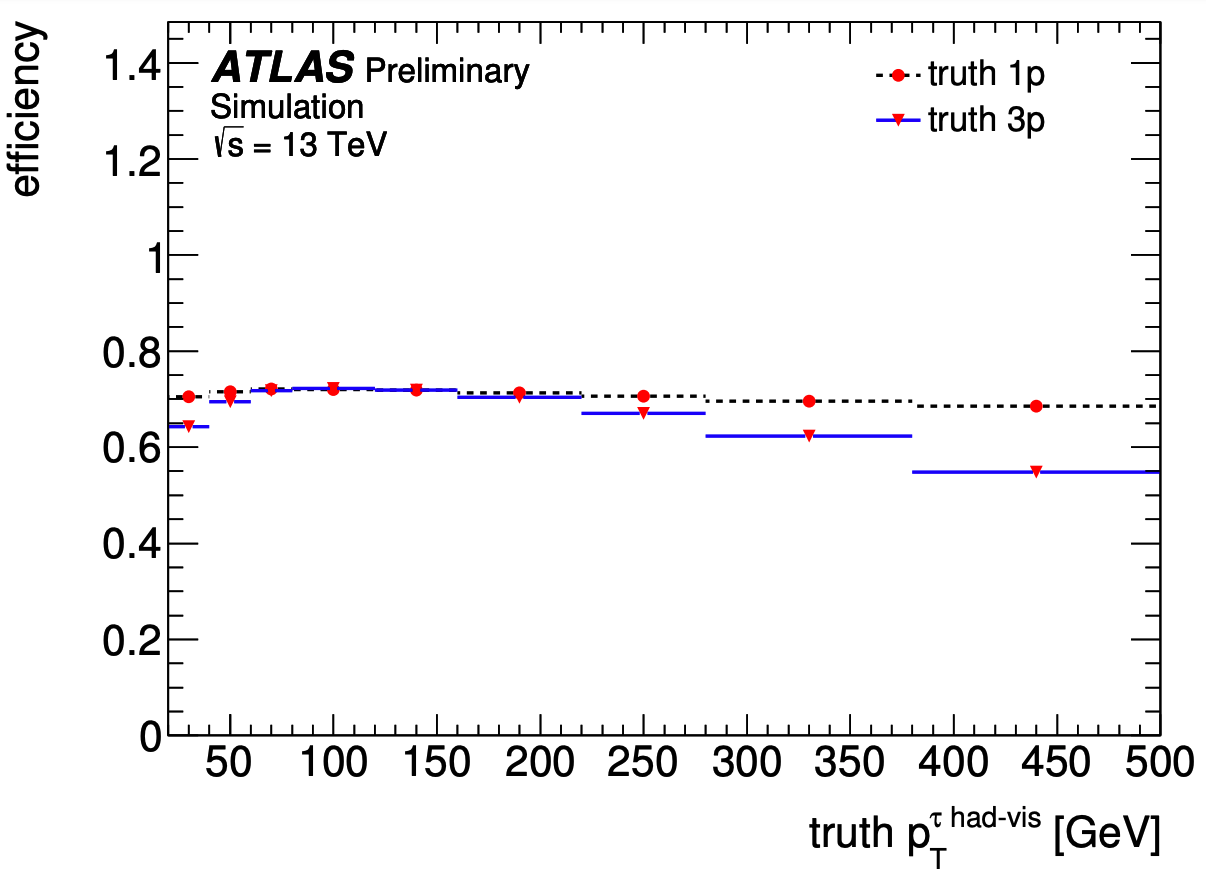
\includegraphics[width=0.5\textwidth]{FakeTau/tau_reco_eff_plt}
%			  \caption{Efficiency for reconstructing the same number of tracks as the number of charged decay products of the tau lepton as a function of visible \htau\ \pt. (taken from~\cite{ATL-PHYS-PUB-2015-045})} 
%			   \label{fig:tau_reco_eff}
%\end{wrapfigure}
%The \htau\ reconstruction efficiency is defined as the fraction of 1-prong (3-prong) \htau\ decays which are reconstructed as a 1-track (3-track) visible \htau\ candidate by the ATLAS detector and reconstruction algorithm divided by the number of true visible \htau\ objects in the event (truth $\tau_{\textrm{had-vis}}$) and identified at truth level using the truth matching method described in more details in Section ~\ref{sec:ffmeth}.
%Figure ~\ref{fig:tau_reco_eff} shows the reconstruction efficiency for 1-prong and 3-prong \htau\ with respect to true visible \htau\ \pt\ ($p_T^{\tau_\textrm{had-vis}}$). 
%The efficiency is relatively constant for 1-prong decays with respect to the transverse momentum of the visible \htau, peaking at around 75\% at $100$ \gev\ with a slow drop towards the higher values of momentum due to two separate effects.
%Very high-\pt\ tau leptons may decay after the first pixel detector and fail the requirement on the number of hits.
%Secondly, the probability of wrongly classifying an electron from photon conversion as a charged hadron from a tau decay also increases with \pt, thus increasing the probability of assigning the incorrect number of charged particles in the tau decay. 
%For the 3-prong decay the efficiency is found to be ranging between 50 - 75 \%. The reduction in efficiency observed for the 3-prong decays in  the low-\pt\ bins is due to the minimum transverse momentum requirement on the charged decay products, and at high-\pt\ the increase collimation of the decay products results in an increased probability of missing a track due to overlapping trajectories.~\cite{ATL-PHYS-PUB-2015-045}

%	\subsection*{Hadronic tau Identification}
%The identification of visible \htau\ candidates to discriminate tau lepton decays from hadronic jet follows the approach described in Reference ~\cite{ATL-PHYS-PUB-2015-045} for Run-1, and the first half of Run-2 (up to 2018), where a \ac{BDT} ~\cite{ATL-PHYS-PUB-2015-045} multivariate technique is used to distinguish between the true visible \htau\ objects for QCD processes. For the second half of Run-2 (2018-onwards) the \ac{BDT}-based tau identification algorithm was superseeded by the \ac{RNN} identification algorithm described in reference~\cite{ATL-PHYS-PUB-2019-033}, which was found to have a rejection power about two times better than the previously used \ac{BDT}-based classifier for any given signal selection efficiency. 
%\begin{figure}[!htb]
%\centering
%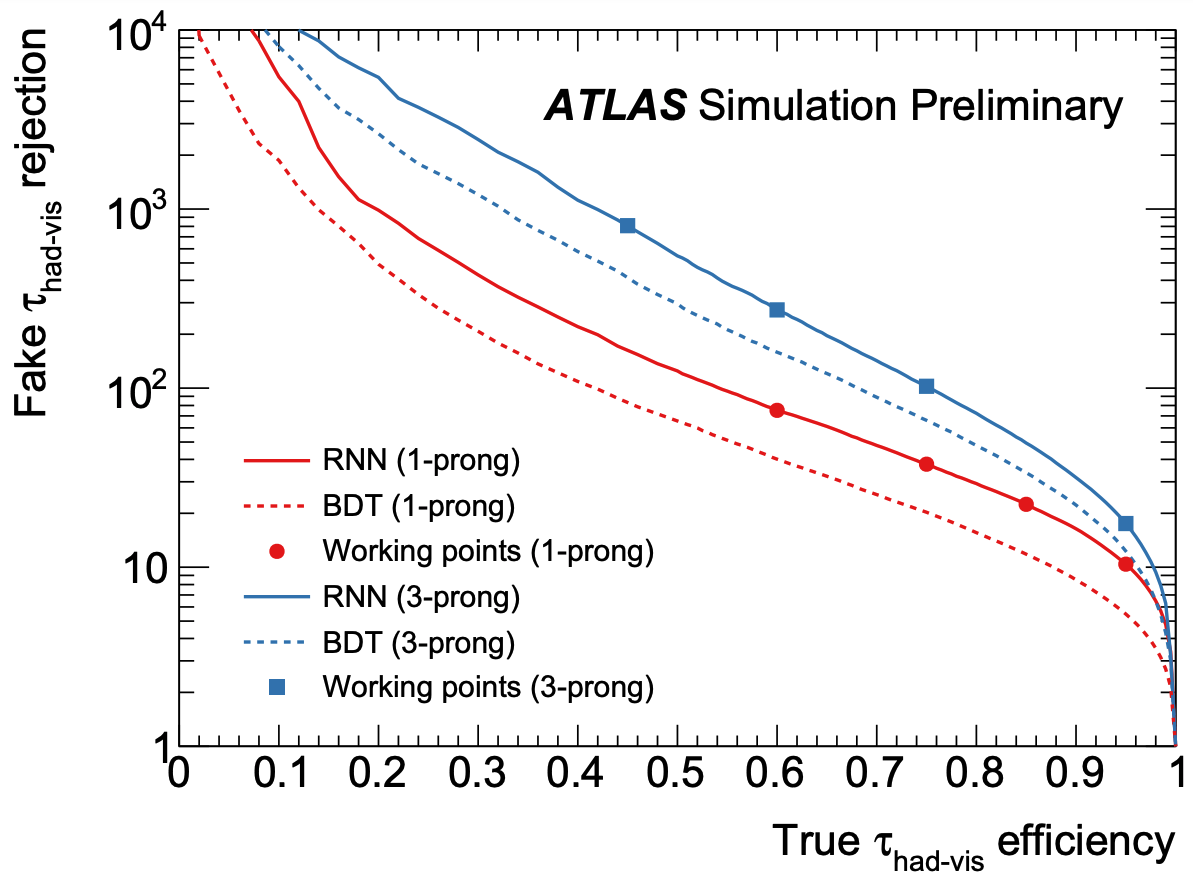
\includegraphics[width=0.75\textwidth]{FakeTau/BDT_vs_RNN}
%\caption{Rejection power for quark and gluon jets misidentified as visible \htau\ (fake visible \htau) depending on the true visible \htau\
%efficiency. Shown are the curves for 1-prong (red) and 3-prong (blue) visible \htau\ candidates using the \ac{RNN}-based (full
%line) and the \ac{BDT}-based (dashed line) identification algorithms. The markers indicate the four defined working
%points \textit{Tight, Medium, Loose and Very loose} with increasing signal selection efficiencies (taken from ~\cite{ATL-PHYS-PUB-2019-033}).}
%\label{fig:BDTvsRNN}
%\end{figure}
%
%The rejection power against misidentified \htau\ as a function of the true visible \htau\ selection efficiency, for both \ac{BDT} and \ac{RNN} classifiers (independently for 1-prong and 3-prong candidates), is shown in Figure ~\ref{fig:BDTvsRNN}.
%Four working points with increasing background rejection (\textit{Very loose}, \textit{Loose}, \textit{Medium} and\textit{Tight}) are used in the physics analyses. The corresponding signal selection efficiencies and rejection powers are given in Table \ref{tab:BDT_RNN_eff}
%\begin{table}[!hbt]
%\label{tab:BDT_RNN_eff}
%\caption{List of defined working points with fixed true visible \htau\ selection efficiencies and the corresponding background rejection factors for misidentified visible \htau\ in dijet events for the \ac{BDT} and \ac{RNN} classifiers (taken from ~\cite{ATL-PHYS-PUB-2019-033}).}
%%\documentclass[10pt]{article}
%\usepackage[usenames]{color} %used for font color
%\usepackage{amssymb} %maths
%\usepackage{amsmath} %maths
%\usepackage[utf8]{inputenc} %useful to type directly diacritic characters
%\begin{document}
%\begin{table}[]
\resizebox{\textwidth}{!}{\begin{tabular}{lcccccc}
\hline 
              & \multicolumn{2}{c}{Signal Efficiency}                     & \multicolumn{2}{c}{Background Rejection BDT}              & \multicolumn{2}{c}{Background Rejection RNN}              \\
Working Point & \multicolumn{1}{c}{1-prong} & \multicolumn{1}{c}{3-prong} & \multicolumn{1}{c}{1-prong} & \multicolumn{1}{c}{3-prong} & \multicolumn{1}{c}{1-prong} & \multicolumn{1}{c}{3-prong} \\ \hline \hline
Tight         & 60\%                        & 45\%                        & 40                          & 400                         & 70                          & 700                         \\
Medium        & 75\%                        & 60\%                        & 20                          & 150                         & 35                          & 240                         \\
Loose         & 85\%                        & 75\%                        & 12                          & 61                          & 21                          & 90                          \\
Very Loose    & 95\%                        & 95\%                        & 5.3                         & 11.2                        & 9.9                         & 16                          \\ \hline
\end{tabular}}
%\end{table}
%
%\end{document}	
%\end{table}
%
%It is important to note that the rejection power for quark and gluon jets misidentified as visible \htau\ objects is strongly dependent on the reconstructed \htau\ \pt (as well more weakly dependent on $\eta$ and \mubar)~\cite{ATL-PHYS-PUB-2019-033}. 
%Figure ~\ref{fig:BDT_RNN_rejection_power} shows the background rejection in dijet events for the \textit{Medium} working point for both \ac{BDT} and \ac{RNN} classifiers as a function of reconstructed \htau\ \pt. The rejection power is found to increase with increasing \pt. 
%	\begin{figure}[!htb]
%		\begin{center}
%			\subbottom[]{
%						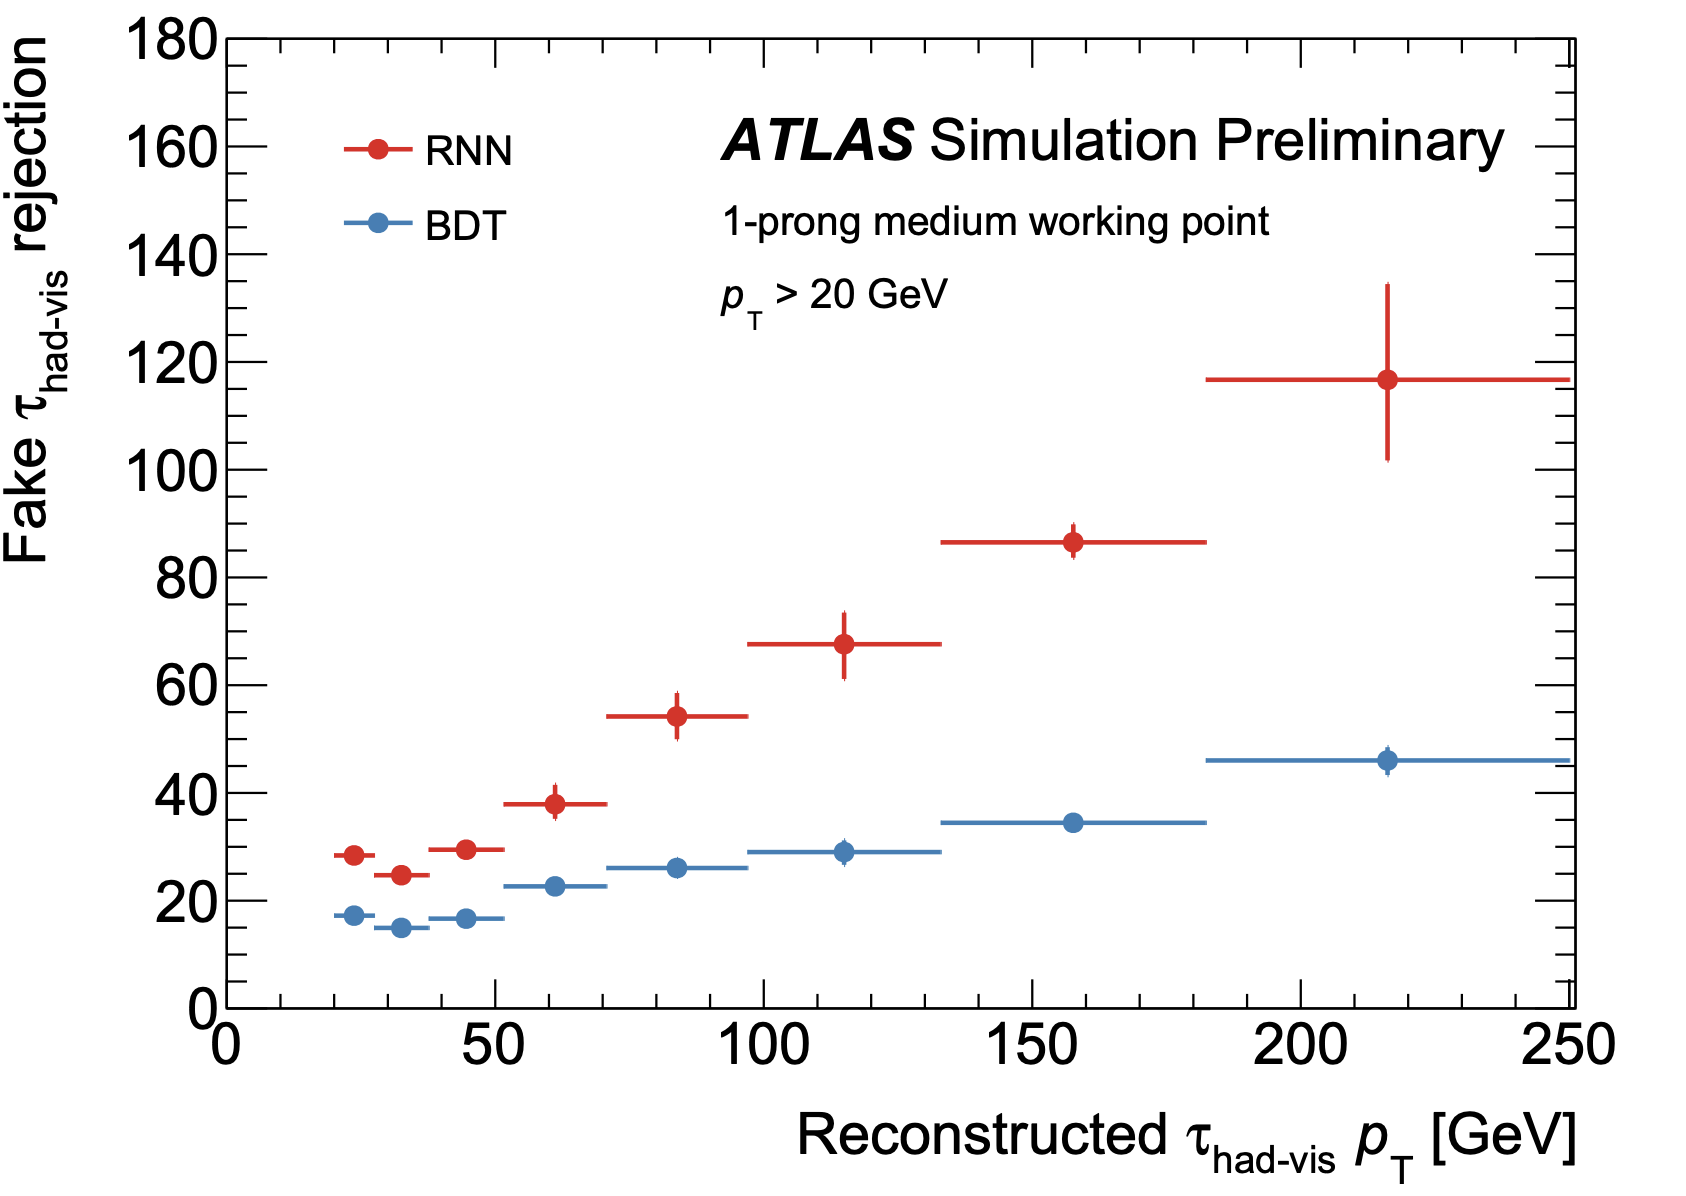
\includegraphics[width=0.45\textwidth]{FakeTau/BDT_RNN_rejection_power_1p}}\hspace{0.05\textwidth}
%			\subbottom[]{
%						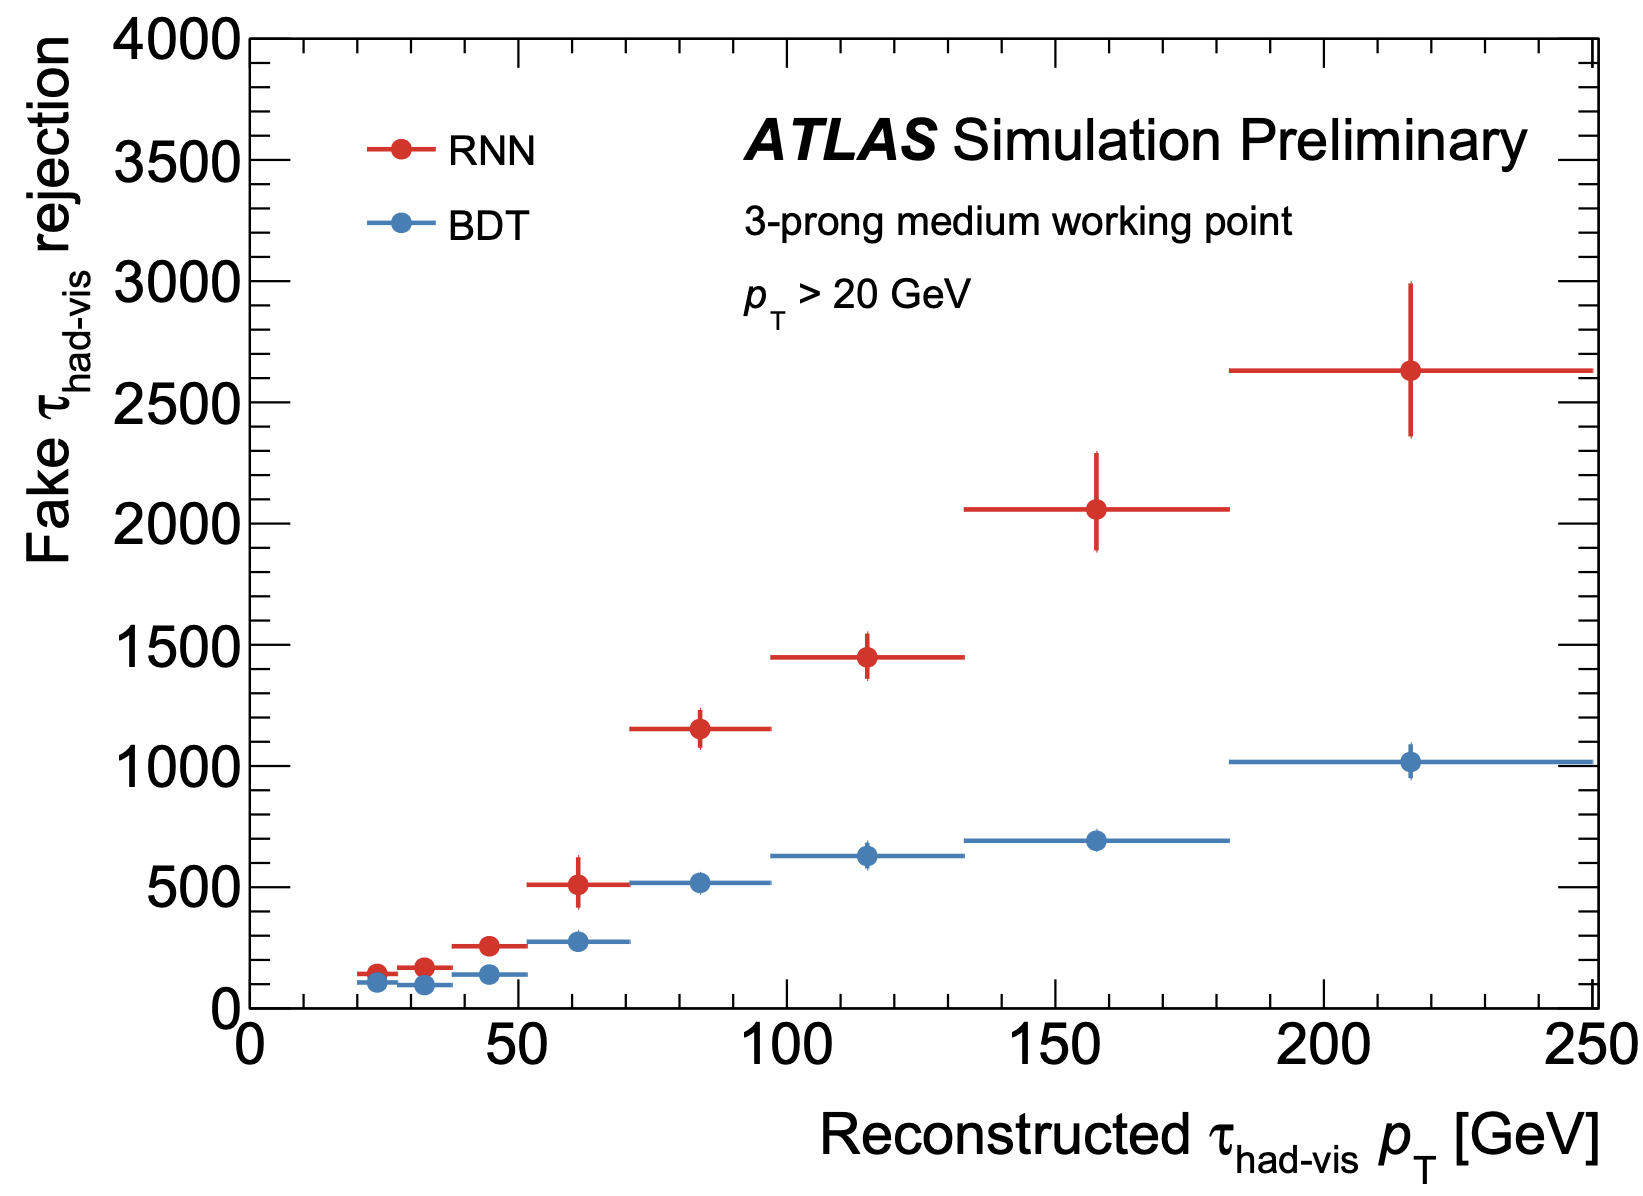
\includegraphics[width=0.45\textwidth]{FakeTau/BDT_RNN_rejection_power_3p}}\hspace{0.05\textwidth}
%		\end{center}
%		\caption{Rejection power for quark and gluon jets misidentified as visible \htau\ (fake visible \htau) for (a) 1-prong and (b) 3-prong as a function of their transverse momentum \pt. The rejection power is shown for the \textit{Medium} working point for both \ac{RNN}-based (red) and \ac{BDT}-based (blue) classifiers. (taken from ~\cite{ATL-PHYS-PUB-2019-033}).}
%		\label{fig:BDT_RNN_rejection_power}
%	\end{figure}

%\begin{wrapfigure}{R}{.5\textwidth}
%		  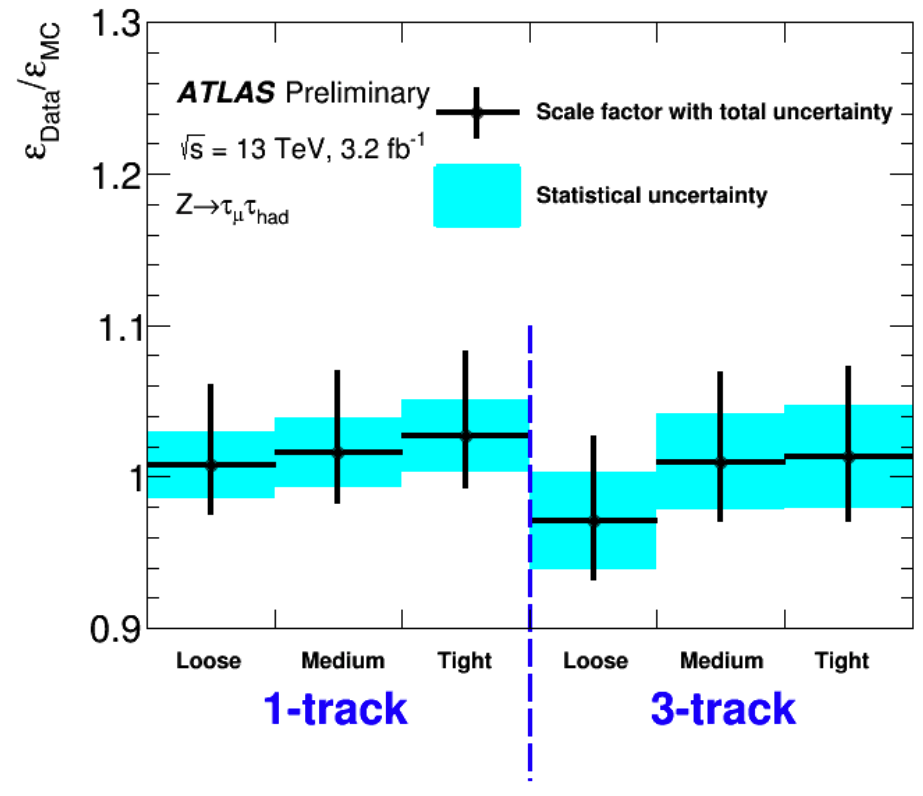
\includegraphics[width=0.5\textwidth]{FakeTau/offline_tau_id_eff}
%			  \caption{The scale factors ($\varepsilon_{Data}$/$\varepsilon_{MC}$) needed to bring the offline tau identification efficiency in simulation ($\varepsilon_{MC}$) to the level observed in data ($\varepsilon_{Data}$) for one track and three track \htau candidates with pT > 20 GeV. The combined systematic and statistical uncertainties are shown. (taken from~\cite{Mitani:2199788}).}
%	\label{fig:offtaueff}
%\end{wrapfigure}
%	
%	Section ~\ref{sec:idtrigtrack} already describes in some detail the algorithm and performance of the inner detector tracking of the tau leptons. More detailed information regarding the algorithms involved in the triggering, reconstructing and identifying tau leptons for data collected during proton-proton collisions at \com\ = 8 TeV  and \com\ = 13 TeV can be found in Ref.~\cite{Aad:2015ydr}and ~\cite{TheATLAScollaboration:2015lks} respectively.
%
%	Figure ~\ref{fig:offtaueff} shows the offline tau identification efficiency measurement for the ratio of efficiency in data ($\varepsilon_{Data}$) to the efficiency in simulation ($\varepsilon_{MC}$), referred to as scale factor, for \htau\ signal to pass a certain level of identification, and are found with 5-6\% precision. Figure ~\ref{fig:tautrigeff} (a) and (b) show the tau trigger efficiencies for low the \pt spectrum for 1 and 3 track \htau objects respectively, measured with 3-20\% precision, while (c) and (d) show the the tau trigger efficiencies for high \pt spectrum for similarly 1 and 3 track \htau objects respectively, measured with 8-14\% precision.
%The tau energy scale shift factors have also been found to be $\alpha=-0.7\%$ $\pm 0.8\%$ (stat)~\cite{Mitani:2199788}
%	\begin{figure}[!htb]
%	\begin{center}
%			 				\subbottom[]{
%								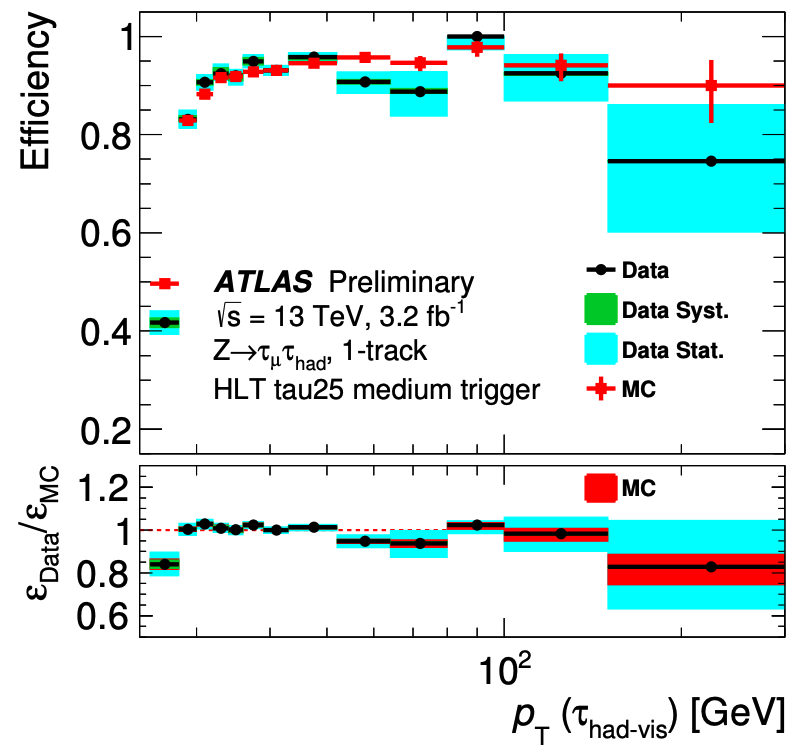
\includegraphics[width=0.45\textwidth]{FakeTau/tau_trig_eff_1p_ztt}}\hspace{0.05\textwidth}
%							\subbottom[]{
%								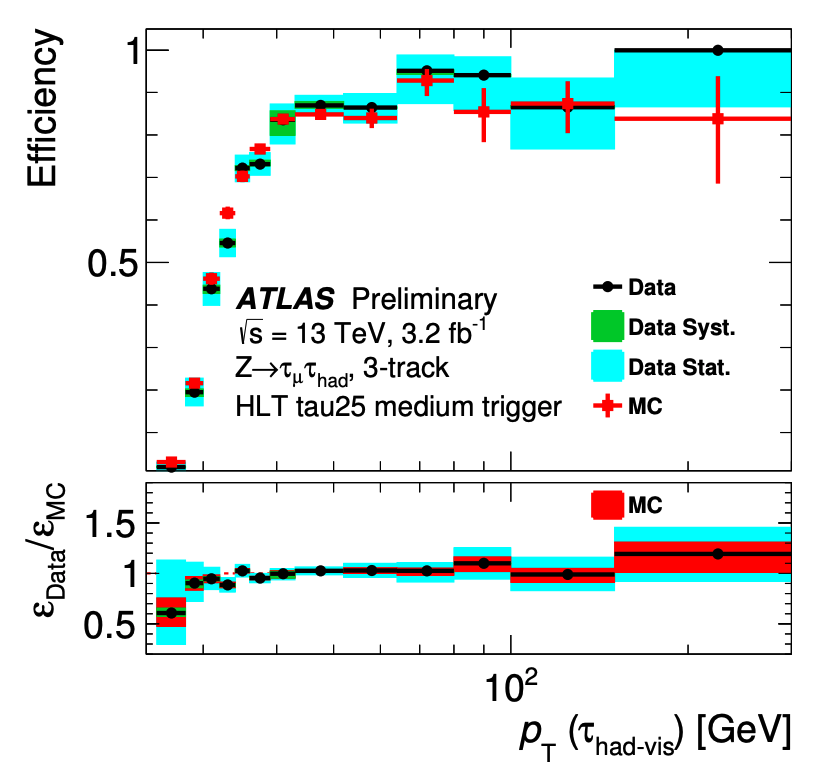
\includegraphics[width=0.45\textwidth]{FakeTau/tau_trig_eff_3p_ztt}}\hspace{0.05\textwidth}
%						\medskip
%							\subbottom[]{
%								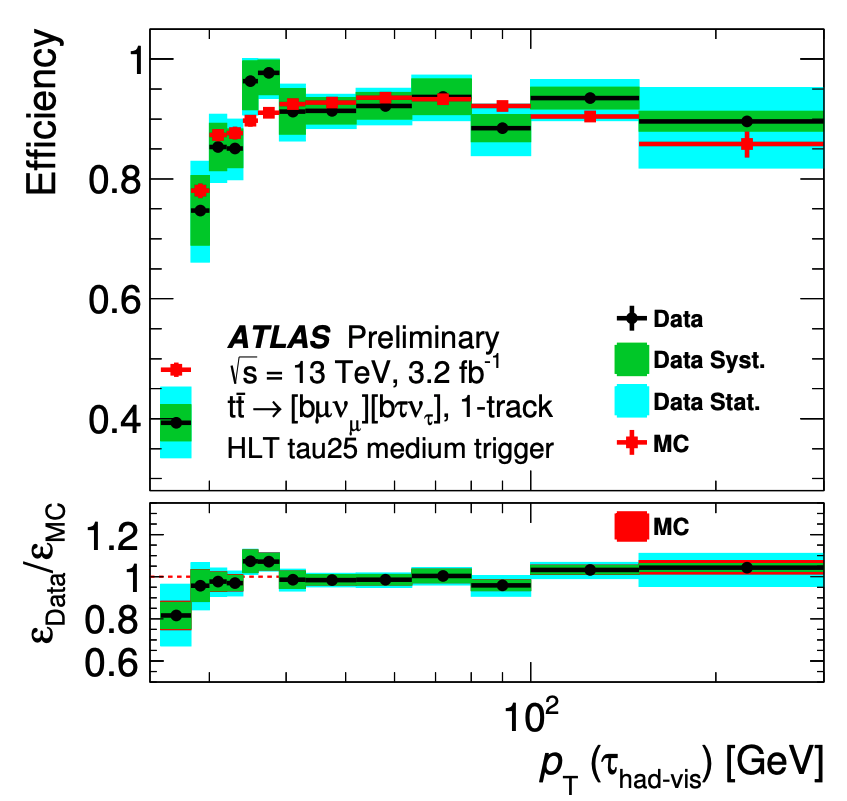
\includegraphics[width=0.45\textwidth]{FakeTau/tau_trig_eff_1p_ttbar}}\hspace{0.05\textwidth}
%							\subbottom[]{
%								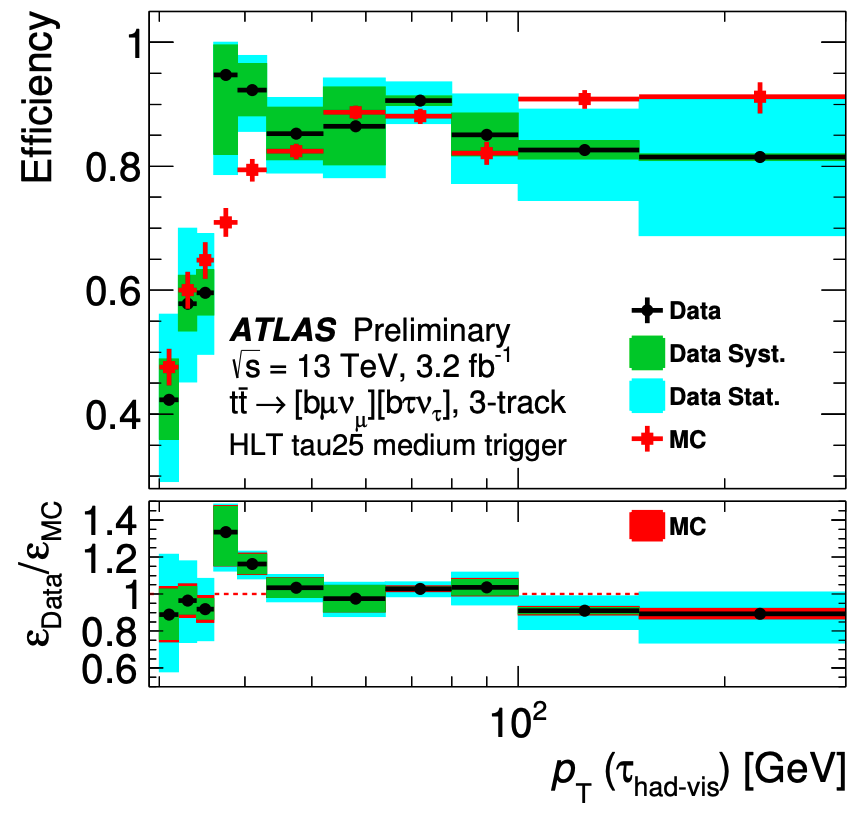
\includegraphics[width=0.45\textwidth]{FakeTau/tau_trig_eff_3p_ttbar}}\hspace{0.05\textwidth}
%	\end{center}
%	\caption{something}
%	\label{fig:tautrigeff}
%	\end{figure}
	
	%Table ~\ref{tab:taueff} summarises the tau performance measurements for the offline identification, energy scale, trigger and electron veto.~\cite{Mitani:2199788} The uncertainties for the offline tau identification, online tau identification and probability of identifying electrons as tau candidates correction factors measurements are approximately 5\% (6\%) for one (three) track, 

	\section{Fake Factor method} \label{sec:ffmeth}
	As shown in the previous section, after the \htau\ identification with either \ac{BDT} or \ac{RNN} techniques, there are still large numbers of misidentified \htau\ objects (\ftau) remaining. 
	Monte Carlo simulations are insufficient to properly model the \ftau\ background with large enough statistics. 
	This is due to the large cross section of jet production at the LHC relative to the $\tau$ production and the subsequent difficulty in modelling jet shower shape and track multiplicity to match that of a true $\tau$ jet.
	
	Data-driven methods, such as the \ac{FF} method described here, are therefore a very powerful tool towards the estimation of \ftau.
	In the \ac{FF} method, a correction factor is applied to data, in a particular \ac{SR}, in order to estimate the \ftau\ background in that region. 
	%Where a SR in this care describes any region used to isolate a physics process of interest. 
	This correction factor normally referred to as Fake Factor (FF) value is measured in dedicated \ac{CR} that is abundant in \ftau, and  is defined as:	
	\begin{equation}
		\textrm{FF}(i)=\frac{N_{\tau_{had}}^{CR\textrm{-data}}(i)}{N_{\textrm{anti}-\tau_{had}}^{CR\textrm{-data}}(i)},
		\label{eq:FF}
	\end{equation}	
	where $N_{\tau_{had}}^{CR}$ is the number of visible \htau\ objects in data that pass the identifier algorithm working point of interest (\ac{BDT} or \ac{RNN}) in the given \ac{CR} and $N_{\textrm{anti}-\tau_{had}}^{CR}$ is the number that fail the same working point of interest, also in data. 
	The index, $i$, refers to the bin where the FF is calculated. Typical choices of binning are in \pt, $\eta$ and number of prongs.
	 Assuming that the SR of interest requires the visible \htau\ objects to pass a given identification work point, the number of \ftau's in that region is then calculated by:
	\begin{equation}
		N_{fakes}^{\tau_{had}}(i) = N_{\textrm{anti}-\tau_{had}}(i)\times FF(i),
		\label{eq:Nfakes}
	\end{equation}
	 where $N_{\textrm{anti}-\tau_{had}}$ is the number of visible \htau\ objects in data that fail the identification working point in the \ac{SR}. 
	% The \ac{SR} is expected to have the same requirements as the nominal SR with the exception of the failed working point selection. 
	 It is important to note that $N_{\tau_{had}}^{CR}$, $N_{\textrm{anti}-\tau_{had}}^{CR}$  and $N_{\textrm{anti}-\tau_{had}}$ have the visible \htau\ truth-matched to true $\tau$'s, $e$'s and $\mu$'s in MC subtracted (as described later), thus transforming equation~\ref{eq:FF} to:
	 \begin{equation}
		\textrm{FF}(i)=\frac{N_{\tau_{had}}^{CR}(\textrm{Data})(i)-N_{\textrm{truth }\tau_{had}}^{CR}(\textrm{MC})(i)}{N_{\textrm{anti}-\tau_{had}}^{CR}(\textrm{Data})(i)-N_{\textrm{truth }\textrm{anti}-\tau_{had}}^{CR}(\textrm{MC})(i)},
		\label{eq:FF-realT}
	\end{equation}
	 where $N_{\textrm{truth }\tau_{had}}^{CR}$ and $N_{\textrm{truth }\textrm{anti}-\tau_{had}}^{CR}$ is the number of truth matched \htau\ object in MC simulations for passing and failing the identification criteria, respectively. The contribution of true $\tau$ events in either category are therefore subtracted. Consequently equation~\ref{eq:Nfakes} can also be re-defined as:
	 \begin{equation}
		N_{fakes}^{\tau_{had}}(i) = (N_{\textrm{anti}-\tau_{had}}(\textrm{Data})(i)-N_{\textrm{anti}-\tau_{had}}(\textrm{MC})(i))\times FF(i),
		\label{eq:Nfakes-realT}
	\end{equation}
	 when subtracting the contribution of real $\tau$'s estimated in MC simulations ($N_{\textrm{anti}-\tau_{had}}(\textrm{MC})$).

	\subsection*{Truth Matching}
	The \htau\ truth-matching procedure is performed by comparing the path of a true $\tau$, $e$ or $\mu$ to that of the visible \htau. If the path coincides, \ie the $\Delta R$\footnote{$\Delta R\,=\,\sqrt{(\Delta\eta)^2+(\Delta\phi)^2}$} between the truth object and the reconstructed visible \htau\ is $<0.2$, then the object is considered truth matched. In the case of multiple truth objects being within a cone of $\Delta R\,<\, 0.2$, the object with the highest \pt\ is chosen.
	 
	\begin{figure}[!hbt]
	\centering
	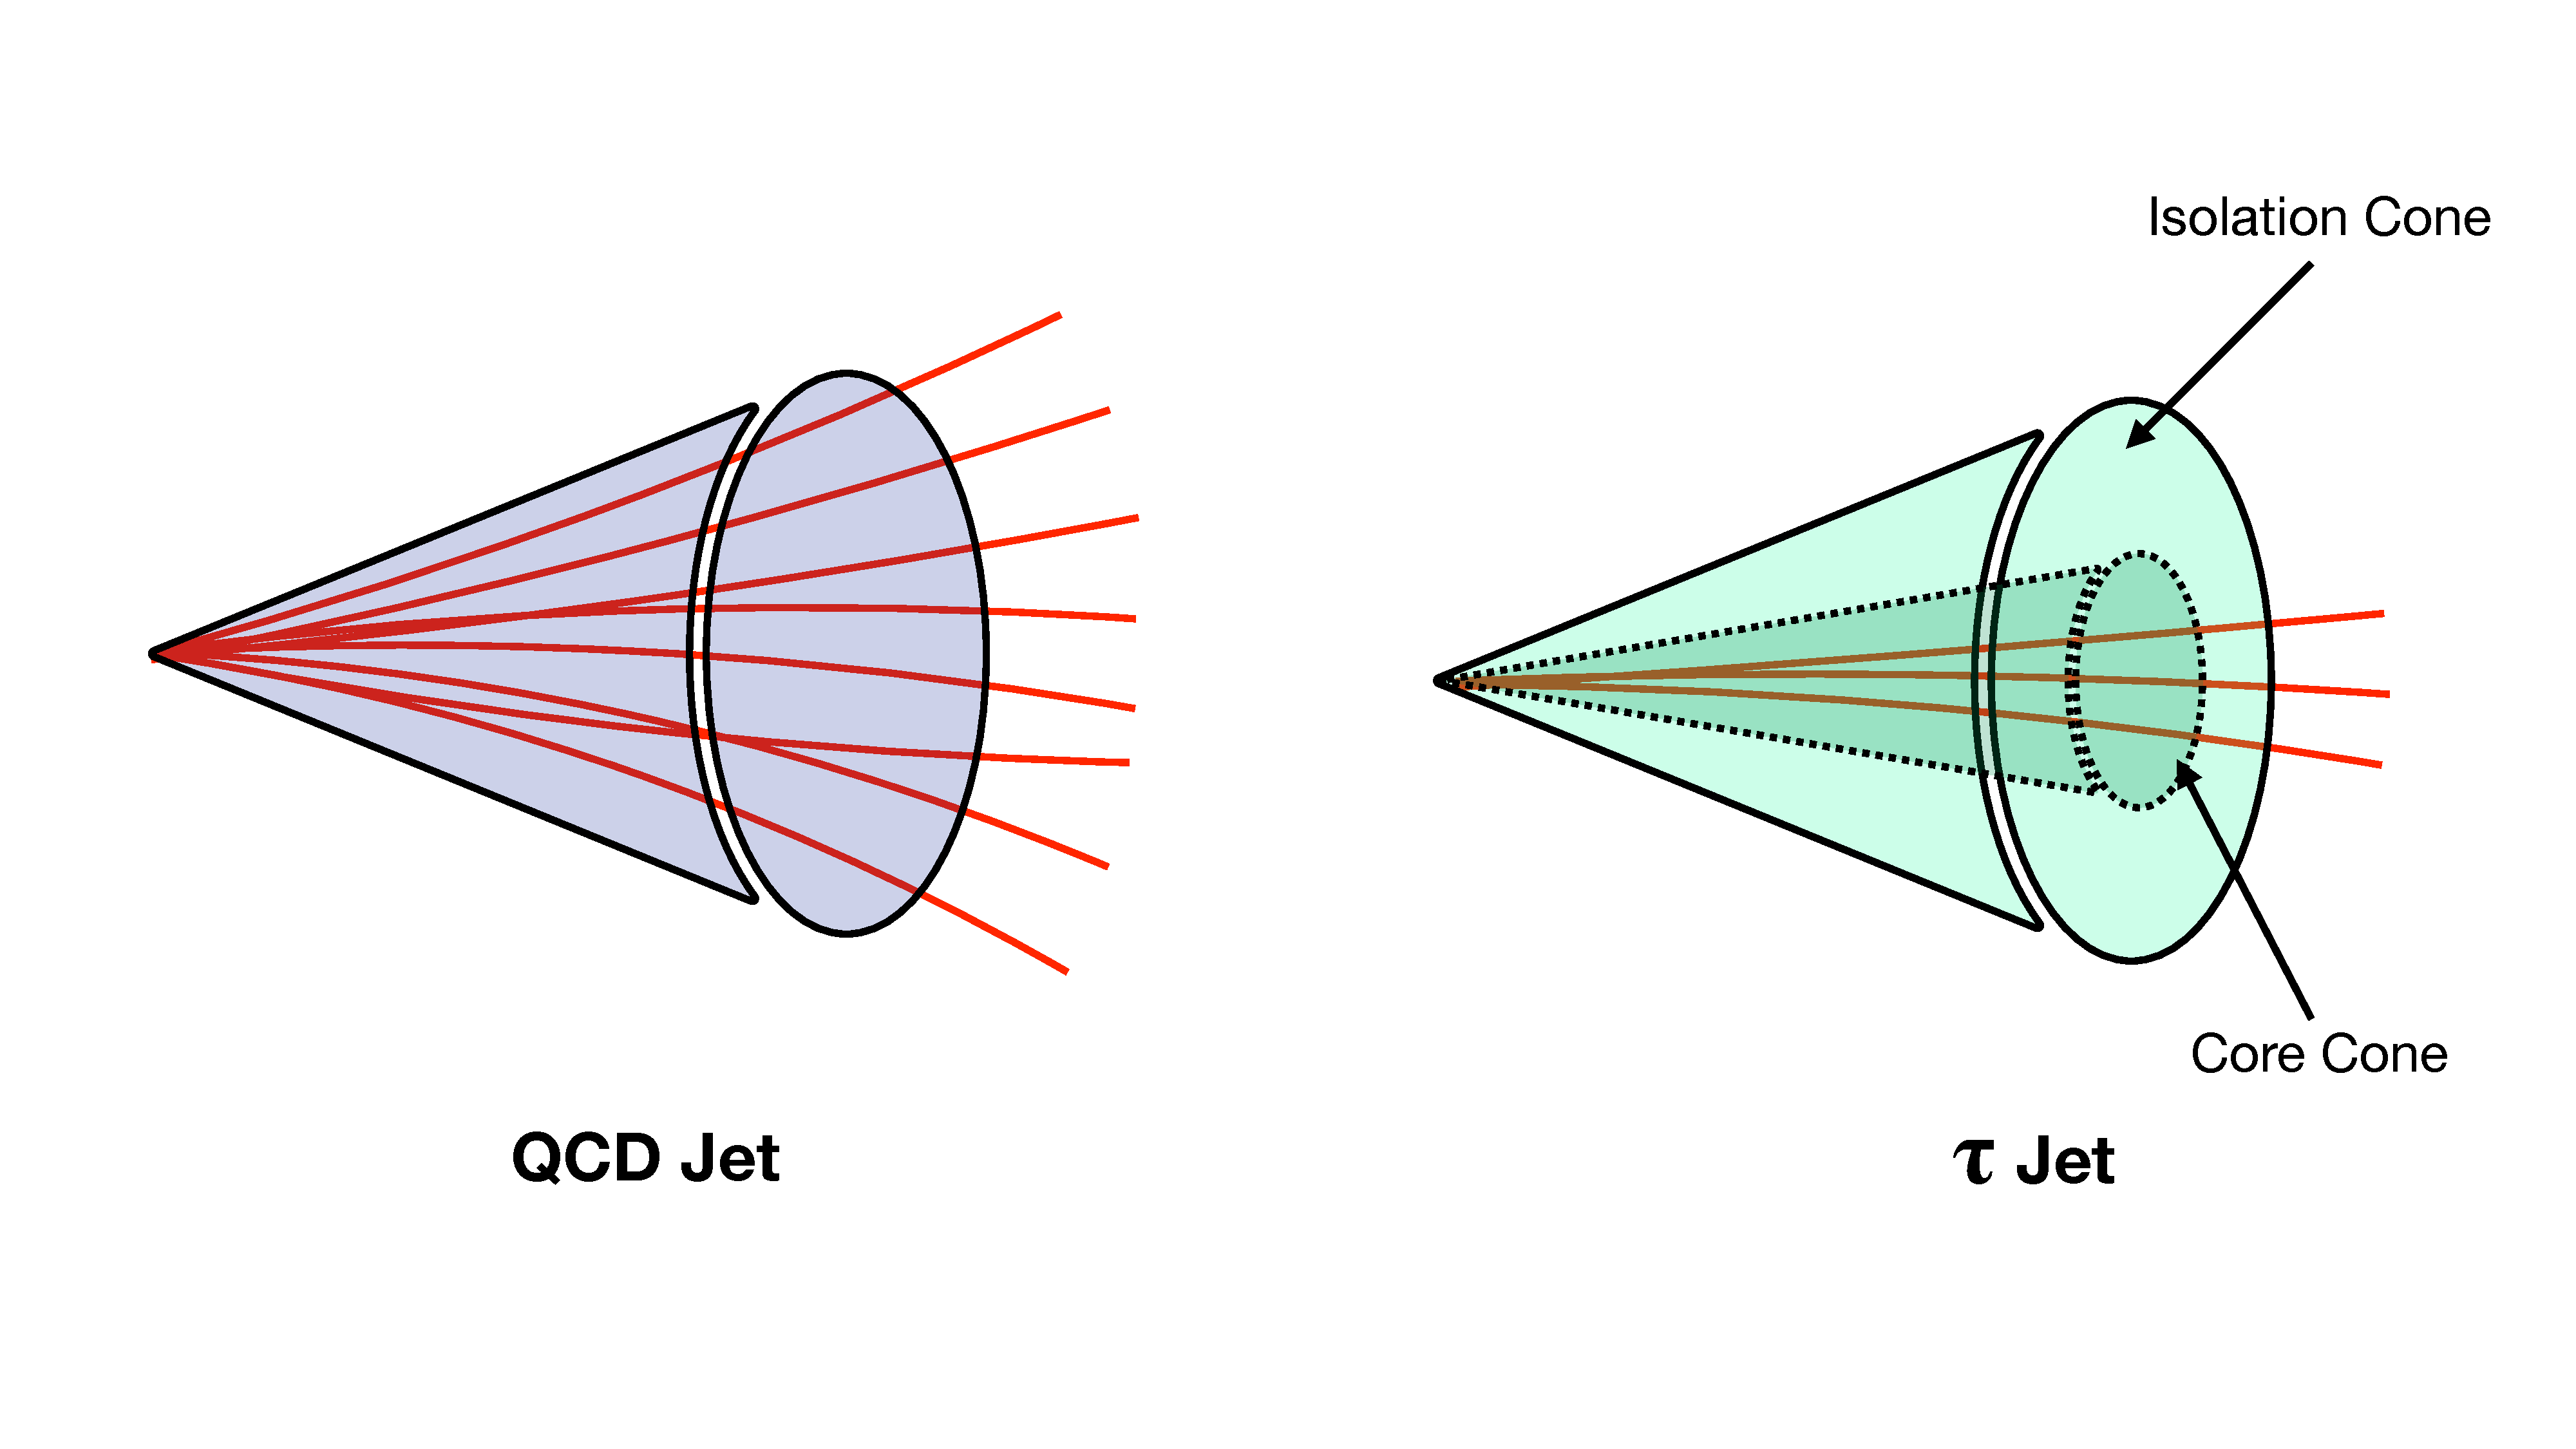
\includegraphics[width=0.9\textwidth]{FakeTau/JetCones}
	\caption{Diagram illustrating the difference in QCD and $tau$ jet cones. $\tau$ jets tend to have one or three charged tracks inside a "core cone" ($\Delta R\,<\,0.2$) and an absence of particles inside a larger "isolation cone"  ($0.2\,<\,\Delta R\,<\,0.4$). QCD jets, on the other hand, generally tend to have more charged tracks in  relatively wide cone.}
	\label{fig:jet_cones}
	\end{figure}		
	Jets are associated to the decay of a visible \htau\ if there are either one or three charged tracks that are within a tight "core cone" of $\Delta R \,\lesssim\,0.2$ inside a larger and relatively void "isolation cone" of $\Delta R \,\lesssim\,0.4$, as depicted in Figure~\ref{fig:jet_cones}. 
	QCD jets tend to have more particles in a relatively wide cone compared to those initiated by $\tau$-decays. It is also important to note that quark-initiated jets tend to be more more narrow and contain less particles than jets initiated by gluons.
	
	The implication of this is that quark- and gluon-initated jets have different probabilities of being reconstructed as \htau. 
	Therefore, different background processes tend to have different quark/gluon compositions. Thus the \ac{FF} value generally need to be derived as a combination of \ac{FF} values from different backgrounds process:
	\begin{equation}
	\textrm{FF}_{comb}\,=\,f_W\textrm{FF}_W\,+\,f_Z\textrm{FF}_Z\,+\,f_{t\bar{t}}\textrm{FF}_{t\bar{t}}\,+\,f_{QCD}\textrm{FF}_{QCD}\,+\cdots,
	\label{eq:ff_comb}
	\end{equation}
	where $f_X$ represent the fraction of background source ($X=W,\,Z,\,t\bar{t},\,QCD,\,\ldots$) in the given region of interest and FF$_X$ is the corresponding FF value for that background in the same region. The combined FF value (FF$_{comb}$) is thus derived by combining all the FF values from the different sources of background. 
	%Jets originating for visible \htau\ decays contain either one or 3 charged tracks inside a cone of $\Delta R\,\lesssim\,0.2$
	\section{Universal Fake Factor method} 
	\label{sec:uniffmeth}
	The \ac{FF} should be measured in a \ac{CR} with similar quark/gluon compositions to the \ac{SR}. This is quite difficult to achieve in practice, although is necessary to correctly apply \ac{FF}s to any particular \ac{SR}. The dependence of the quark- and gluon-initiated jet composition in an arbitrary region can be studied by considering the \ac{FF} of pure quark and pure gluon samples. In this case, jets initiated from quarks and gluons would be defined as miss-identified visible \htau's which fail a particular identification criteria working point. If we assume there are no other objects that can initiate a jet (and neglecting the difference in light and heavy flavoured quark-initiated jets)%, although more on this will be discussed in section ~\ref{subsec:FTTFquark})
, the \ac{FF} can be written as a function of the quark fraction:
	\begin{equation}
	\textrm{FF}(q_f)\,=\,q_f\textrm{FF}_q+(1-q_f)\textrm{FF}_g,
	\label{eq:FF_qf}
	\end{equation}		
	where $q_f$ is the fraction of quark-initiated jets in the sample, FF$_q$ is the \ac{FF} of a pure quark and FF$_g$ is the \ac{FF} of a pure gluon sample. If it is assumed that jets can only be initiated by quarks or gluons then:
	\begin{equation}
		1=q_f+g_f,
	\end{equation}		 
	 where $g_f$ is the fraction of gluon-initiated jets in the sample.
	 
	 \begin{figure}[!hbt]
	 \centering
	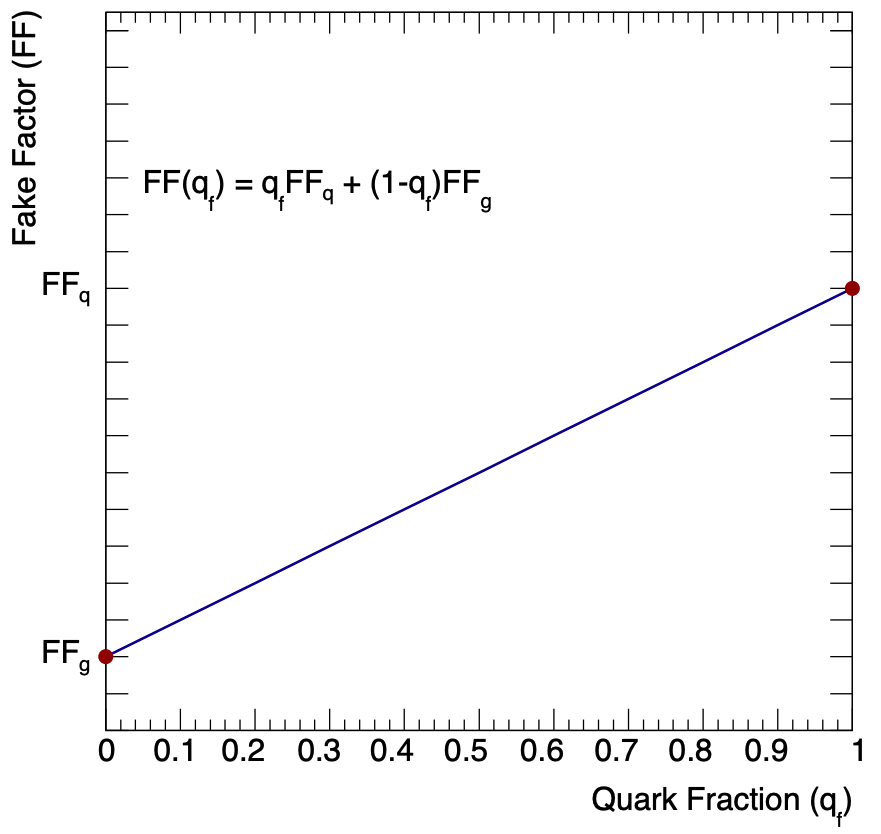
\includegraphics[width=0.55\textwidth]{FakeTau/FF_qf1}
	\caption{Illustration of linear dependence of FF on the quark fraction, $q_f$, given the relationship $\textrm{FF}\,=\,q_f\textrm{FF}_q\,+\,(1-q_f)\textrm{FF}_g$. The points at the extremes show the \ac{FF} for a pure quark or pure gluon sample (FF$_q$ FF$_g$ respectively).}
	 \label{fig:FF_qf1}
	 \end{figure}
	Figure~\ref{fig:FF_qf1} shows an illustration representing the FF as a function of $q_f$.
	It is clear that any pure quark or pure gluon region will have fixed values of \ac{FF}, represented in the illustration by FF$_q$ and FF$_g$, respectively.	
	% It is possible to determine the FF for any arbitrary region by knowing the pure quark and gluon FFs.
	However, the pure quark and gluon FFs are not directly measurable quantities in data, but the functional relationship between of the FF and $q_f$ can be determined in data by interpolation. 
	
	If two arbitrary regions are considered, where the \ac{FF}s are written as:
	\begin{equation}
	\textrm{FF}_1\,=\,q_1\textrm{FF}_q+(1-q_1)\textrm{FF}_g,
	\end{equation}
	\begin{equation}
	\textrm{FF}_2\,=\,q_2\textrm{FF}_q+(1-q_2)\textrm{FF}_g,
	\end{equation}
	then FF$_q$ and FF$_g$ can be expresses analytically using the above system of equations:
	\begin{equation}
	\textrm{FF}_q\,=\frac{(1-q_2)\textrm{FF}_1-(1-q_1)\textrm{FF}_2}{q_2-q1},
	\label{eq:FFq}	
	\end{equation}
	and
	\begin{equation}
	\textrm{FF}_g\,=\frac{q_2\textrm{FF}_1-q_1\textrm{FF}_2}{q_2-q1},
	\label{eq:FFg}	
	\end{equation}
	where FF$_1$ and FF$_2$ are measured as described in Section~\ref{sec:ffmeth} using equation~\ref{eq:FF}:
	\begin{equation}
	\label{eq:FF1}
	\textrm{FF}_1\,=\,\frac{N_{\tau_{had}}^{CR_1}}{N_{\textrm{anti}-\tau_{had}}^{CR_1}},
	\end{equation}
	and 
	\begin{equation}
	\label{eq:FF2}
	\textrm{FF}_2\,=\,\frac{N_{\tau_{had}}^{CR_2}}{N_{\textrm{anti}-\tau_{had}}^{CR_2}}.
	\end{equation}
	For any arbitrary \ac{SR} the anti-ID region (\ie\ the same \ac{SR} selection but with the \htau\ identification criteria flipped so that only the events for which the \htau\ fails the identification criteria pass) can be used to derive the appropriate \ac{FF}. Thus, the \ac{FF} can be defined as: 
	\begin{equation}
	\textrm{FF}_{SR}\,=\,q_{SR}\textrm{FF}_q+(1-q_{SR})\textrm{FF}_g,
	\label{eq:FF_SR}
	\end{equation}
	where FF$_{SR}$ is the FF value for this \ac{SR}-like region and FF$_q$ and FF$_g$ are given by equations~\ref{eq:FFq} and ~\ref{eq:FFg} respectively. 
	The \ac{SR}-like region \ac{FF} can be thus be re-written in terms of the \ac{FF} for the two arbitrary regions FF$_1$ and FF$_2$:
	\begin{equation}
	\textrm{FF}_{SR}\,=\,q_{SR}\frac{(1-q_2)\textrm{FF}_1-(1-q_1)\textrm{FF}_2}{q_2-q1}+(1-q_{SR})\frac{q_2\textrm{FF}_1-q_1\textrm{FF}_2}{q_2-q1},
	\end{equation}
	making the FF$_{SR}$ value dependent only on three unknown quantities: $q_1$, $q_2$ and $q_{SR}$, which are the quark fractions for the arbitrary regions 1, 2 and SR respectively.
	Therefore, by deriving the \ac{FF} values of two regions (one gluon and one quark abundant), as well as their corresponding quark fraction it is possible, in tern, to determine the \ac{FF} value for any given \ac{SR}.  
	Figure~\ref{fig:FF_qf2} illustrates this procedure along the linear dependence of FF to $q_f$ for arbitrary regions 1, 2 and SR.
	 The \ac{SR} quark fraction $q_{SR}$ is determined by a fit to quark and gluons derived in \ac{MC} template to data, explained in more details in Section~\ref{sec:TFFT}.
	\begin{figure}[!hbt]
	 \centering
	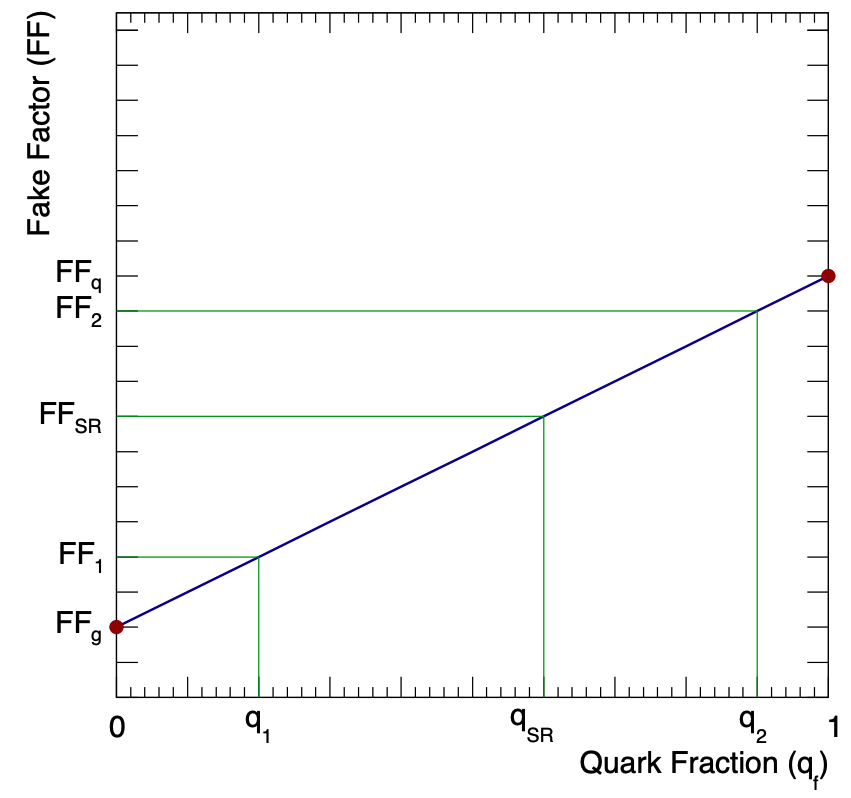
\includegraphics[width=0.55\textwidth]{FakeTau/FF_qf2}
	\caption{Illustration of the interpolation of FF$_{SR}$ using pure quark/gluon FF, thus allowing the determination of FF uniquely by analytically calculating FF$_q$ and FF$_g$.}
	 \label{fig:FF_qf2}
	 \end{figure}
	
%	Figure ~\ref{fig:FF_qf2} illustrates this procedure along the linear dependence of FF to $q_f$ for arbitrary 1, 2 and SR regions.
%	Equation ~\ref{eq:FF_SR} can therefore be re-written as: 
%	\begin{equation}
%	\textrm{FF}_{SR}\,=\,q_{SR}\frac{(1-q_2)\textrm{FF}_1-(1-q_1)\textrm{FF}_2}{q_2-q1}+(1-q_{SR})\frac{q_2\textrm{FF}_1-q_1\textrm{FF}_2}{q_2-q1},
%	\end{equation}
%	and thus be only dependent on three unknown quantities: $q_1$, $q_2$ and $q_{SR}$, which are the three quark fractions of interest.
	
	\subsection*{Jet Width}
	\label{jet_width}
	The quark fraction cannot be calculated directly from data, as individual partons are not seen or reconstructed by the \ac{ATLAS} detector.
	The quark fraction must thus be derived in \ac{MC} using a template method, \ie\ where a \textit{discriminating variable} is used to discriminate between different types of partons. 
	The truth-matching method is thus used to identify the \htau\ objects that are truth-matched to quark and gluon-initiated jets. These objects are then parametrised using a variable with good quark/gluon separation. 
	
	A variable found to have well-suited separation between quarks and gluons is the jet width. 
	The jet width is a \pt -weighted $\Delta R$ of the objects associated to the jet:
	\begin{equation} 
	j\,=\,\frac{\Sigma_i\Delta R^i p_T^i}{\Sigma_i	p_T^i},
	\label{eq:jet_width}
	\end{equation}
	where $i$ is the number of objects that constitute the reconstructed jet. 
	The jet width can be calculated from the calorimeter-based \ac{LC} topo-cluster~\cite{Aad_2017} jets that seed the visible \htau, which in the text will be referred to as calo-based jet width.	
	

	This definition is quite sensitive to proton-proton interactions per bunch crossings (referred to in text as pile-up and denoted by $\mu$)~\cite{Aad_2012}. 
	It was found that the calo-jet based track width was suffering from significant mis-modelling in the MC due to the incorrect modelling of pileup jets in the samples.
	 It thus became impossible to use this particular variable for discrimination despite it having such good sensitivity to quark and gluon-initiated jets. 
	
	Due to this, a track-based jet width was explored instead. 
	The track-based jet width is calculated using the same jet width equation described above (equation~\ref{eq:jet_width}), but only considers tracks associated to the seeded jet that: 
	  %by looping of the tracks associated to a seed jet and:
	\begin{itemize}
		\item Have \pt\ $>\,1000$ MeV
		\item Are associated to the primary vertex 
	\end{itemize}
	 If no tracks fulfil these two requirements, then the jet width value is set to -1. Therefore, track-based jet width values of -1 tend to be associated to pileup jets, which do not come from the interaction's primary vertex.

Some examples of jet width distributions are shown in Figure~\ref{fig:jet_width_diff} for several different \ac{MC} samples. These plots show the normalised quark and gluon calo-based (top) and track-based (bottom) jet widths for Z+jets (left) and Dijets (right) MC16a samples. 
To produce these distributions the reconstructed jet-faking \htau\ was truth-matched to its corresponding parton.
The templates use \htau\ candidates that fail the \textit{Medium} \ac{BDT} working point and have a minimum \ac{BDT} score of 0.005. 
As mentioned above, there is reasonable quark gluon separation in both samples and for both calo-based and track-based jet widths. 
The relatively lower number of gluons observed in the track-based jet width distribution compared to what is found when looking at the calo-based distribution is due to the higher number of gluons that have a track-based jet width value of -1, shown in the plot by the first bin (underflow).
	 \begin{figure}[!htb]
	\begin{center}
			 				\subbottom[]{
								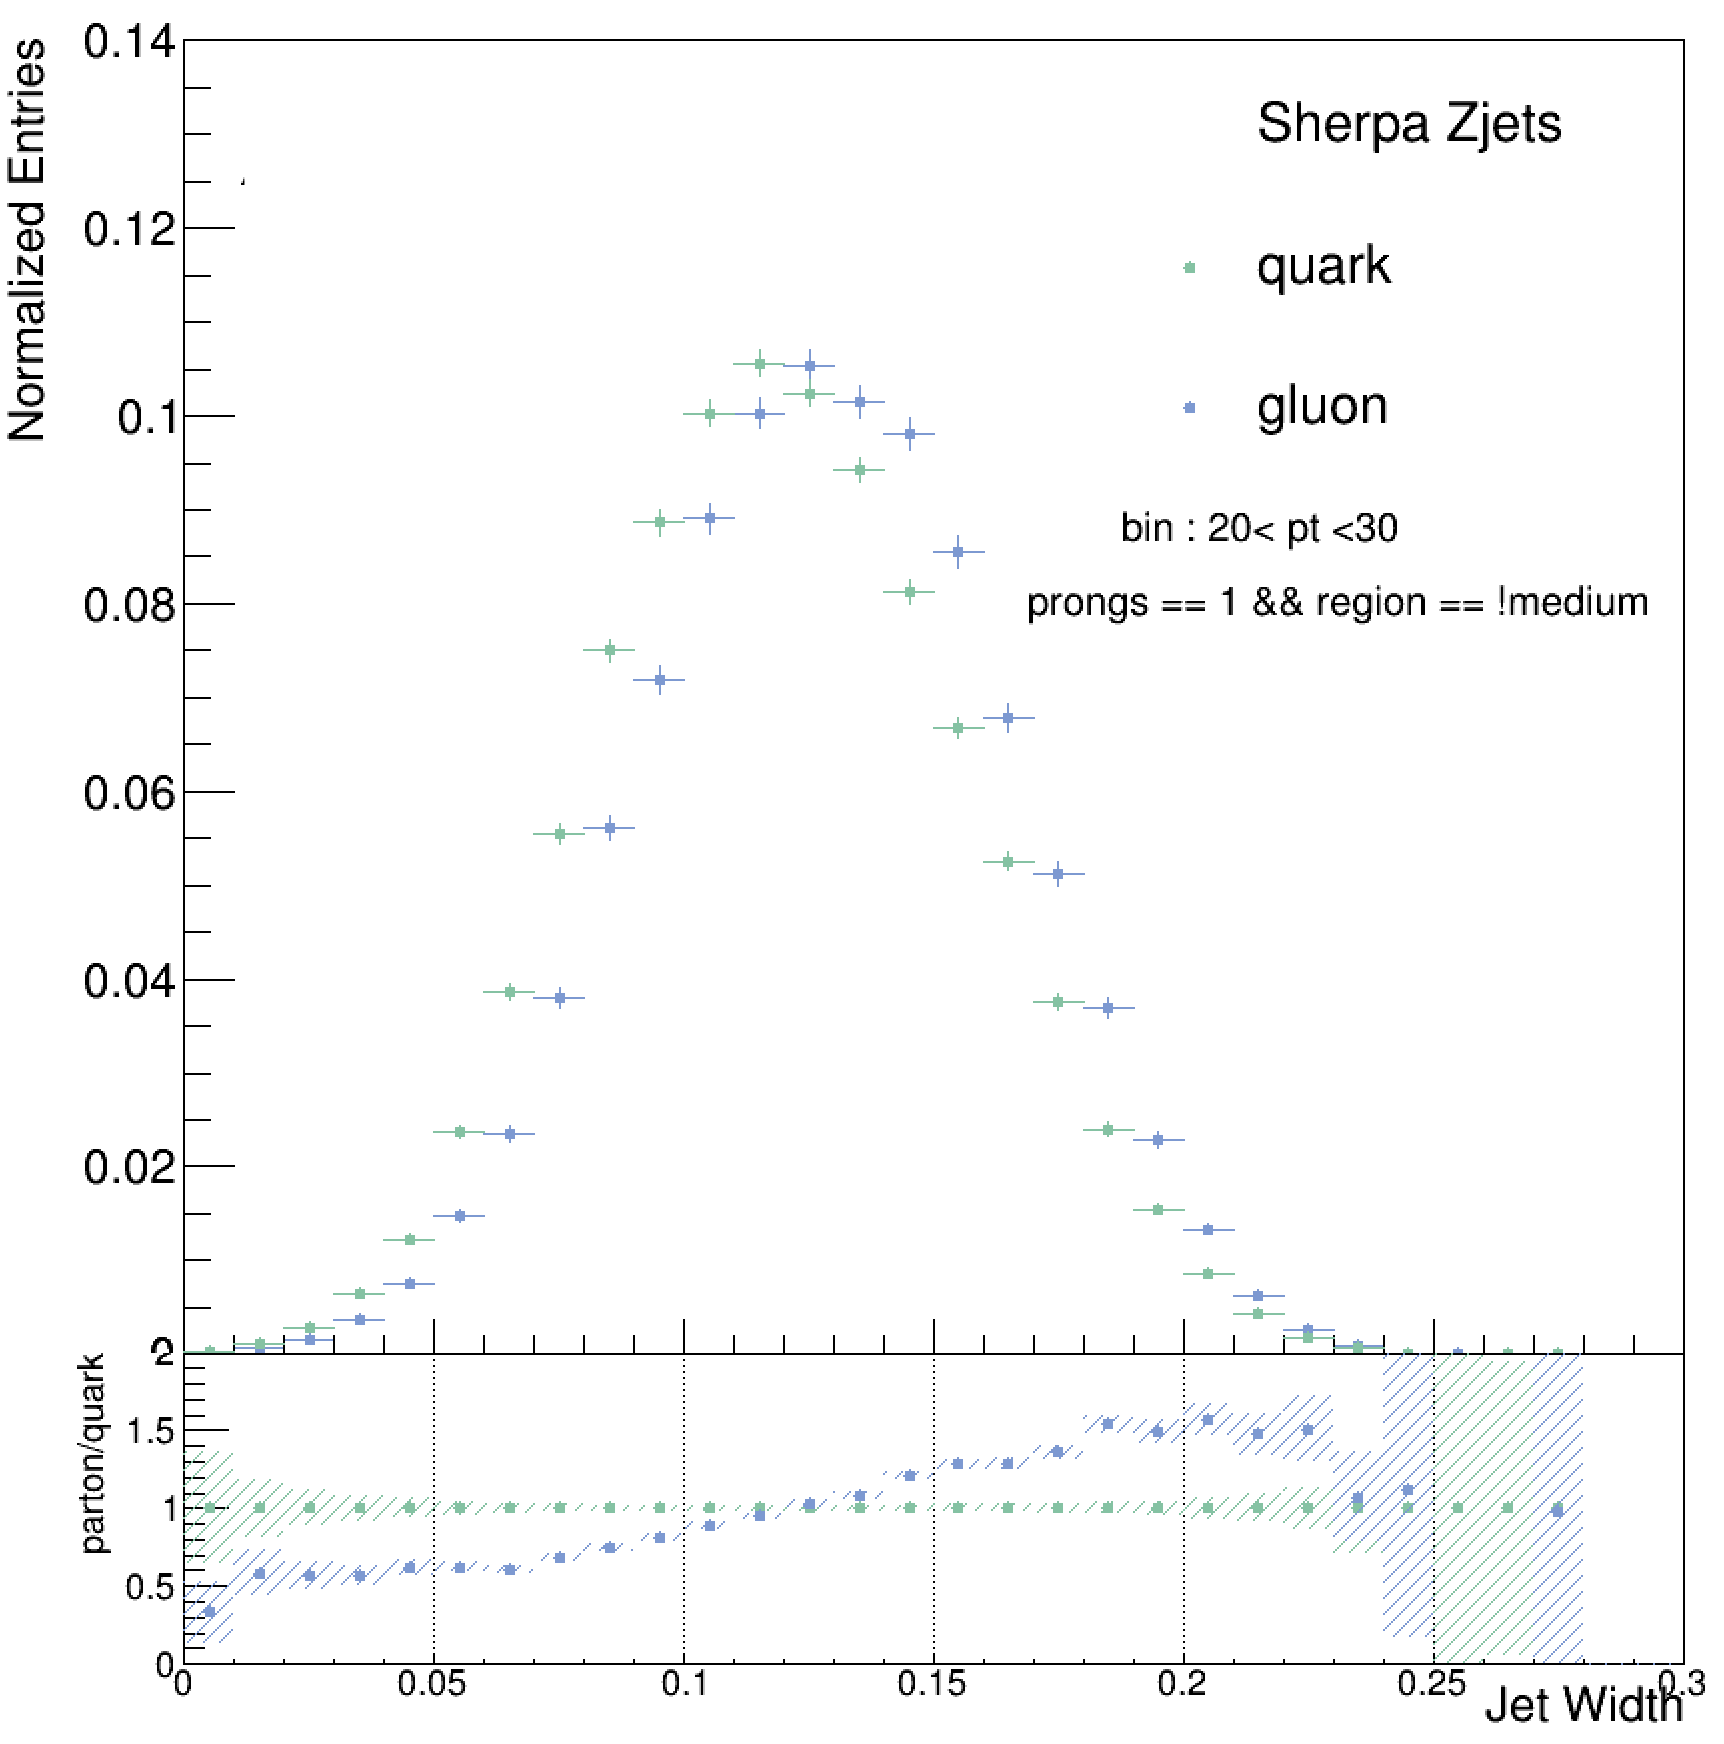
\includegraphics[width=0.4\textwidth]{FakeTau/Jet_width_Zjets}}\hspace{0.05\textwidth}
							\subbottom[]{
								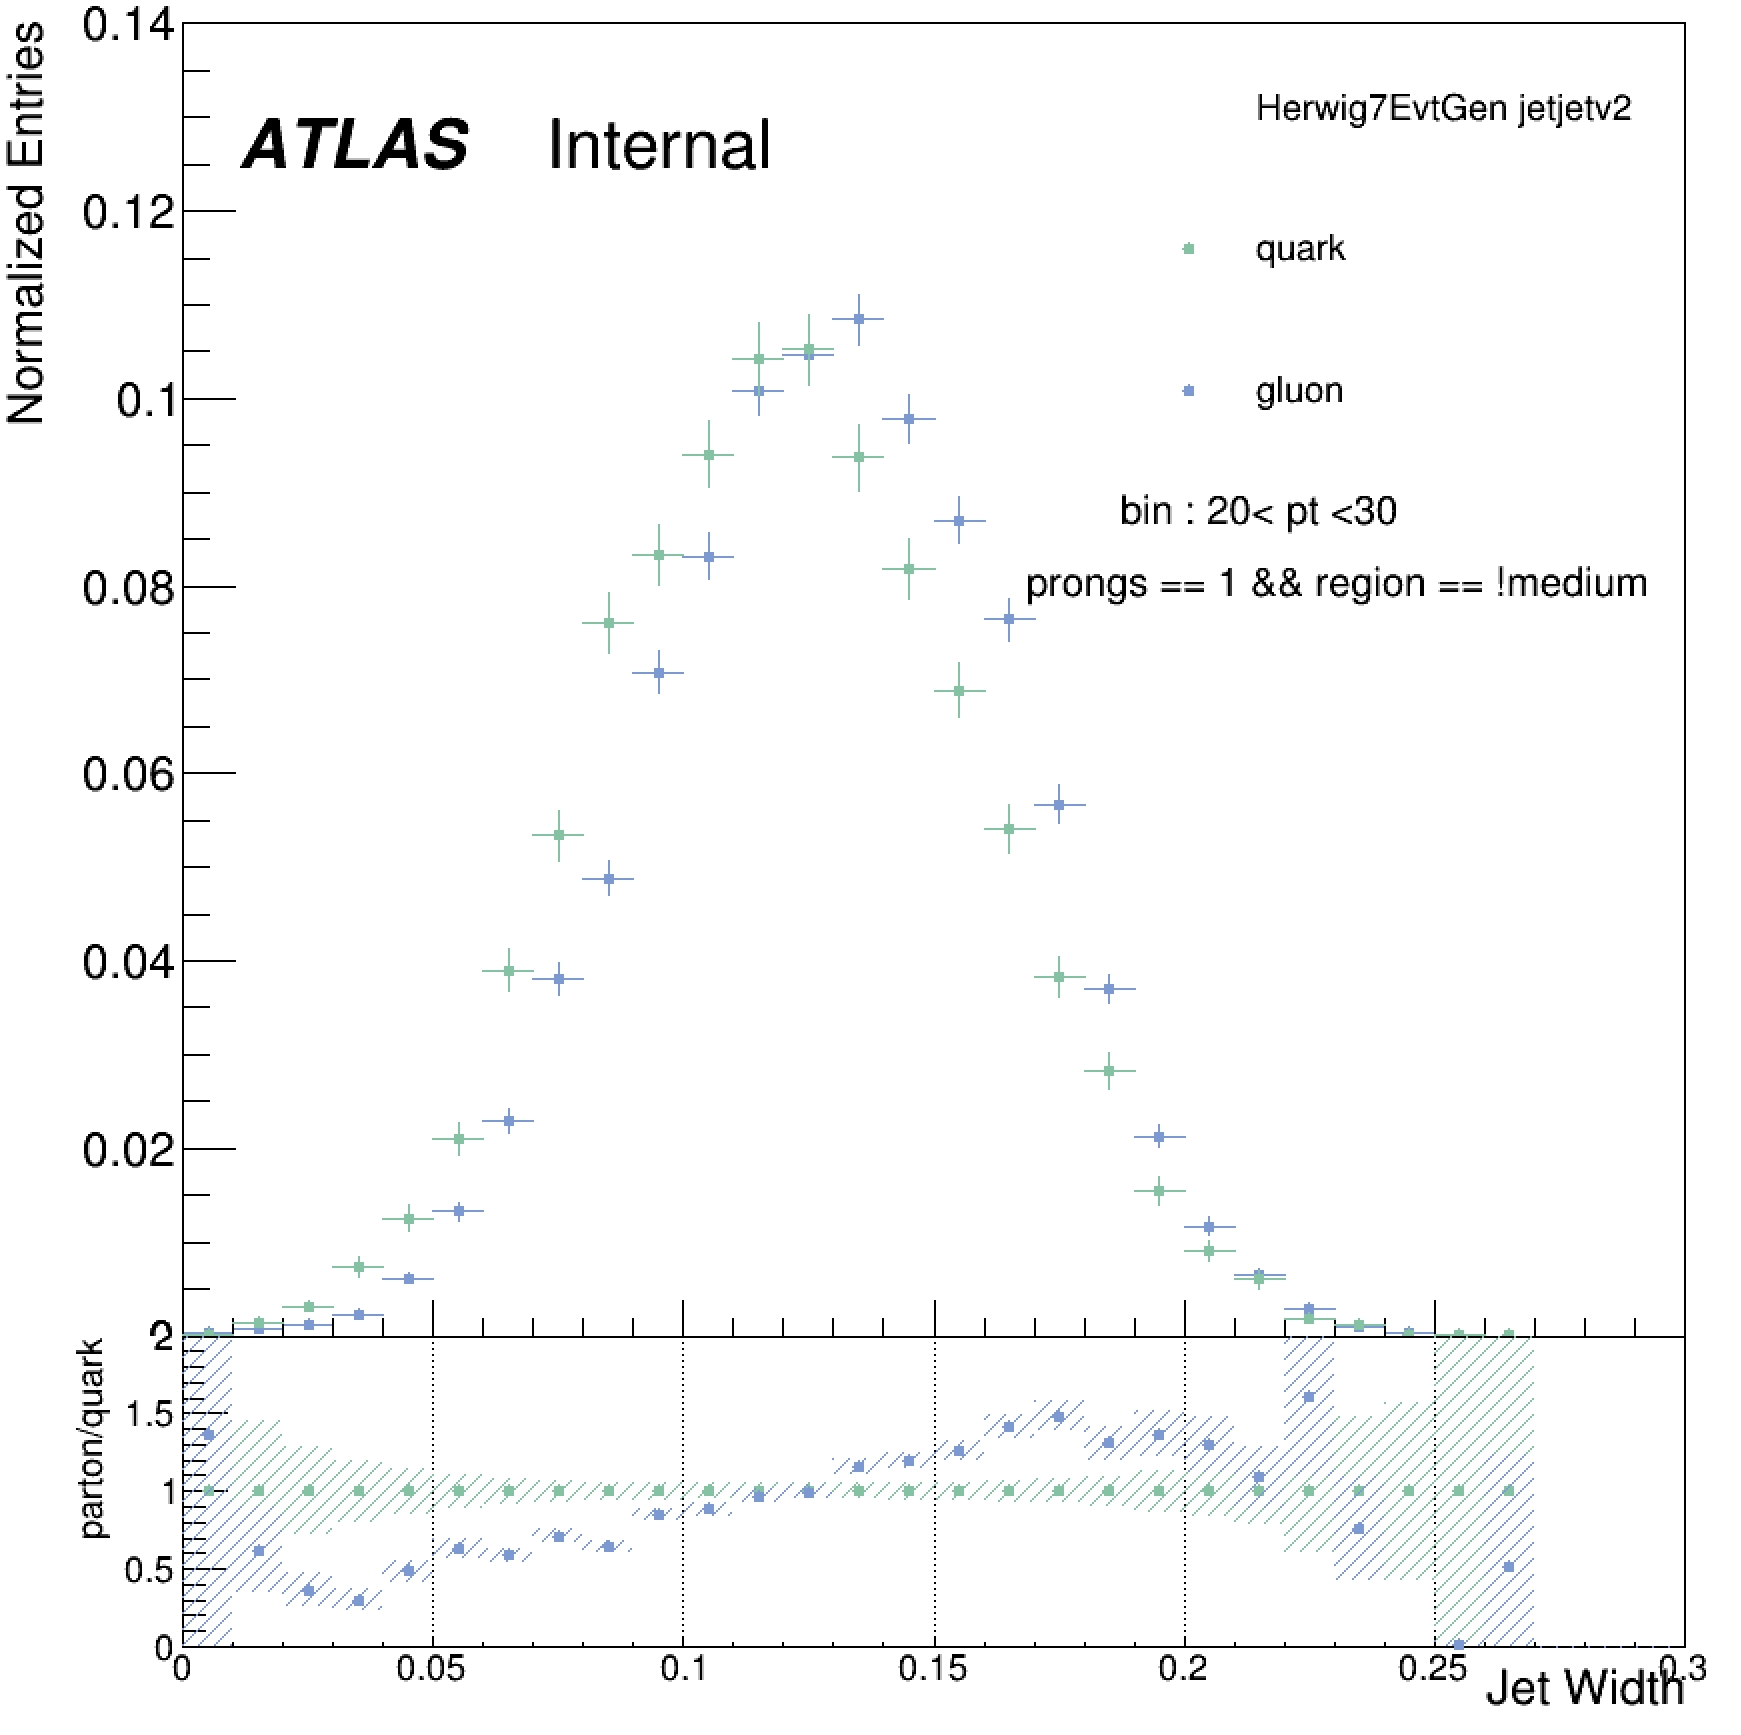
\includegraphics[width=0.4\textwidth]{FakeTau/Jet_width_Dijets}}\hspace{0.05\textwidth}
							\subbottom[]{
								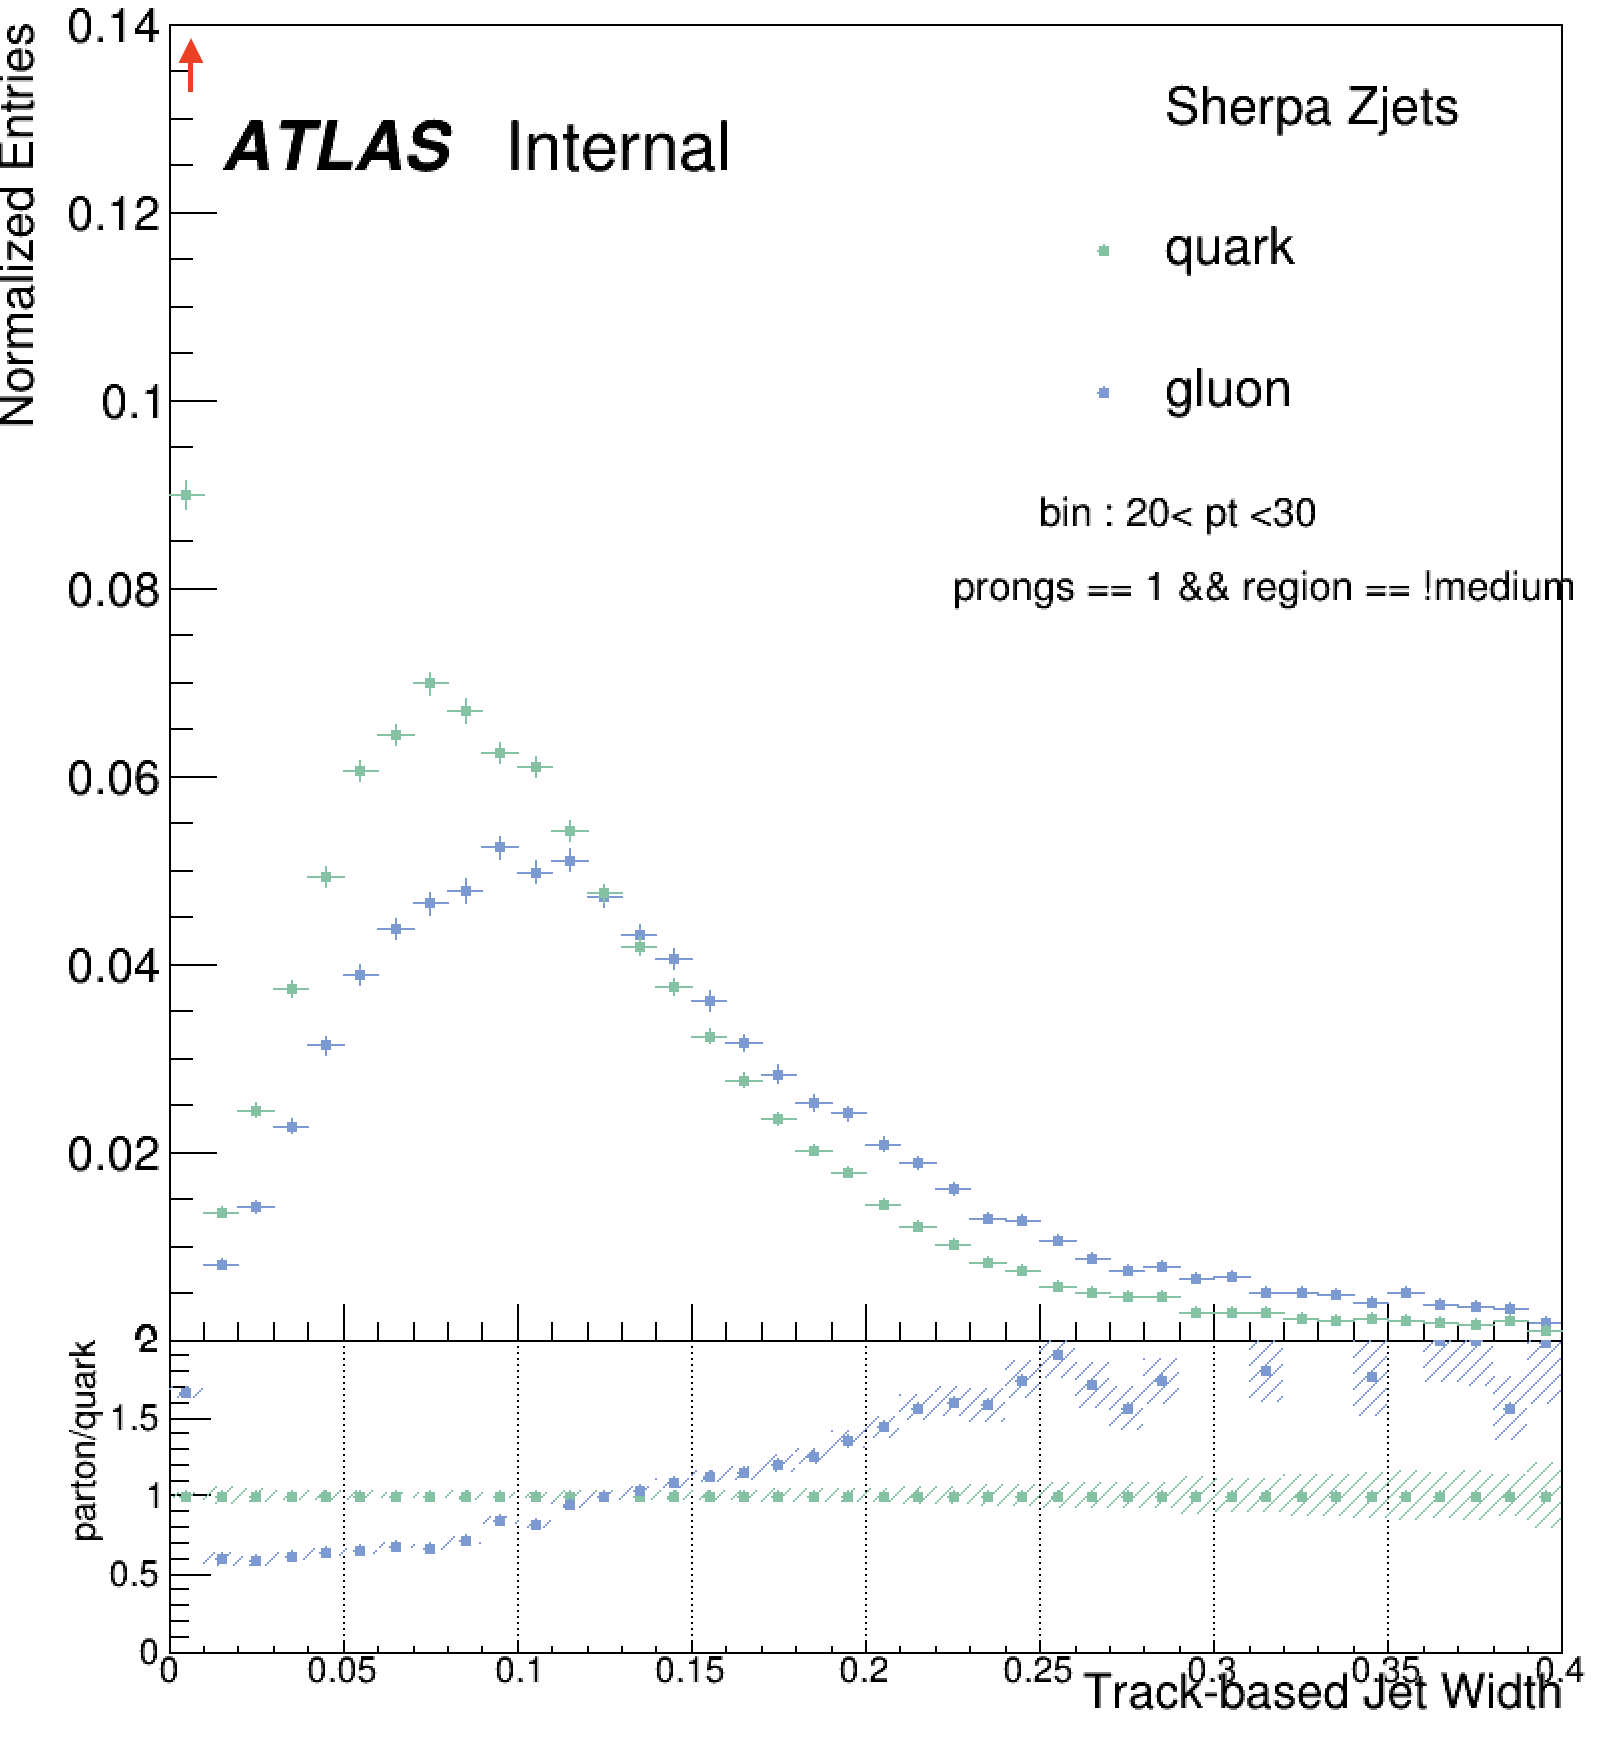
\includegraphics[width=0.4\textwidth]{FakeTau/Track_based_jet_width_Zjets}}\hspace{0.05\textwidth}
							\subbottom[]{
								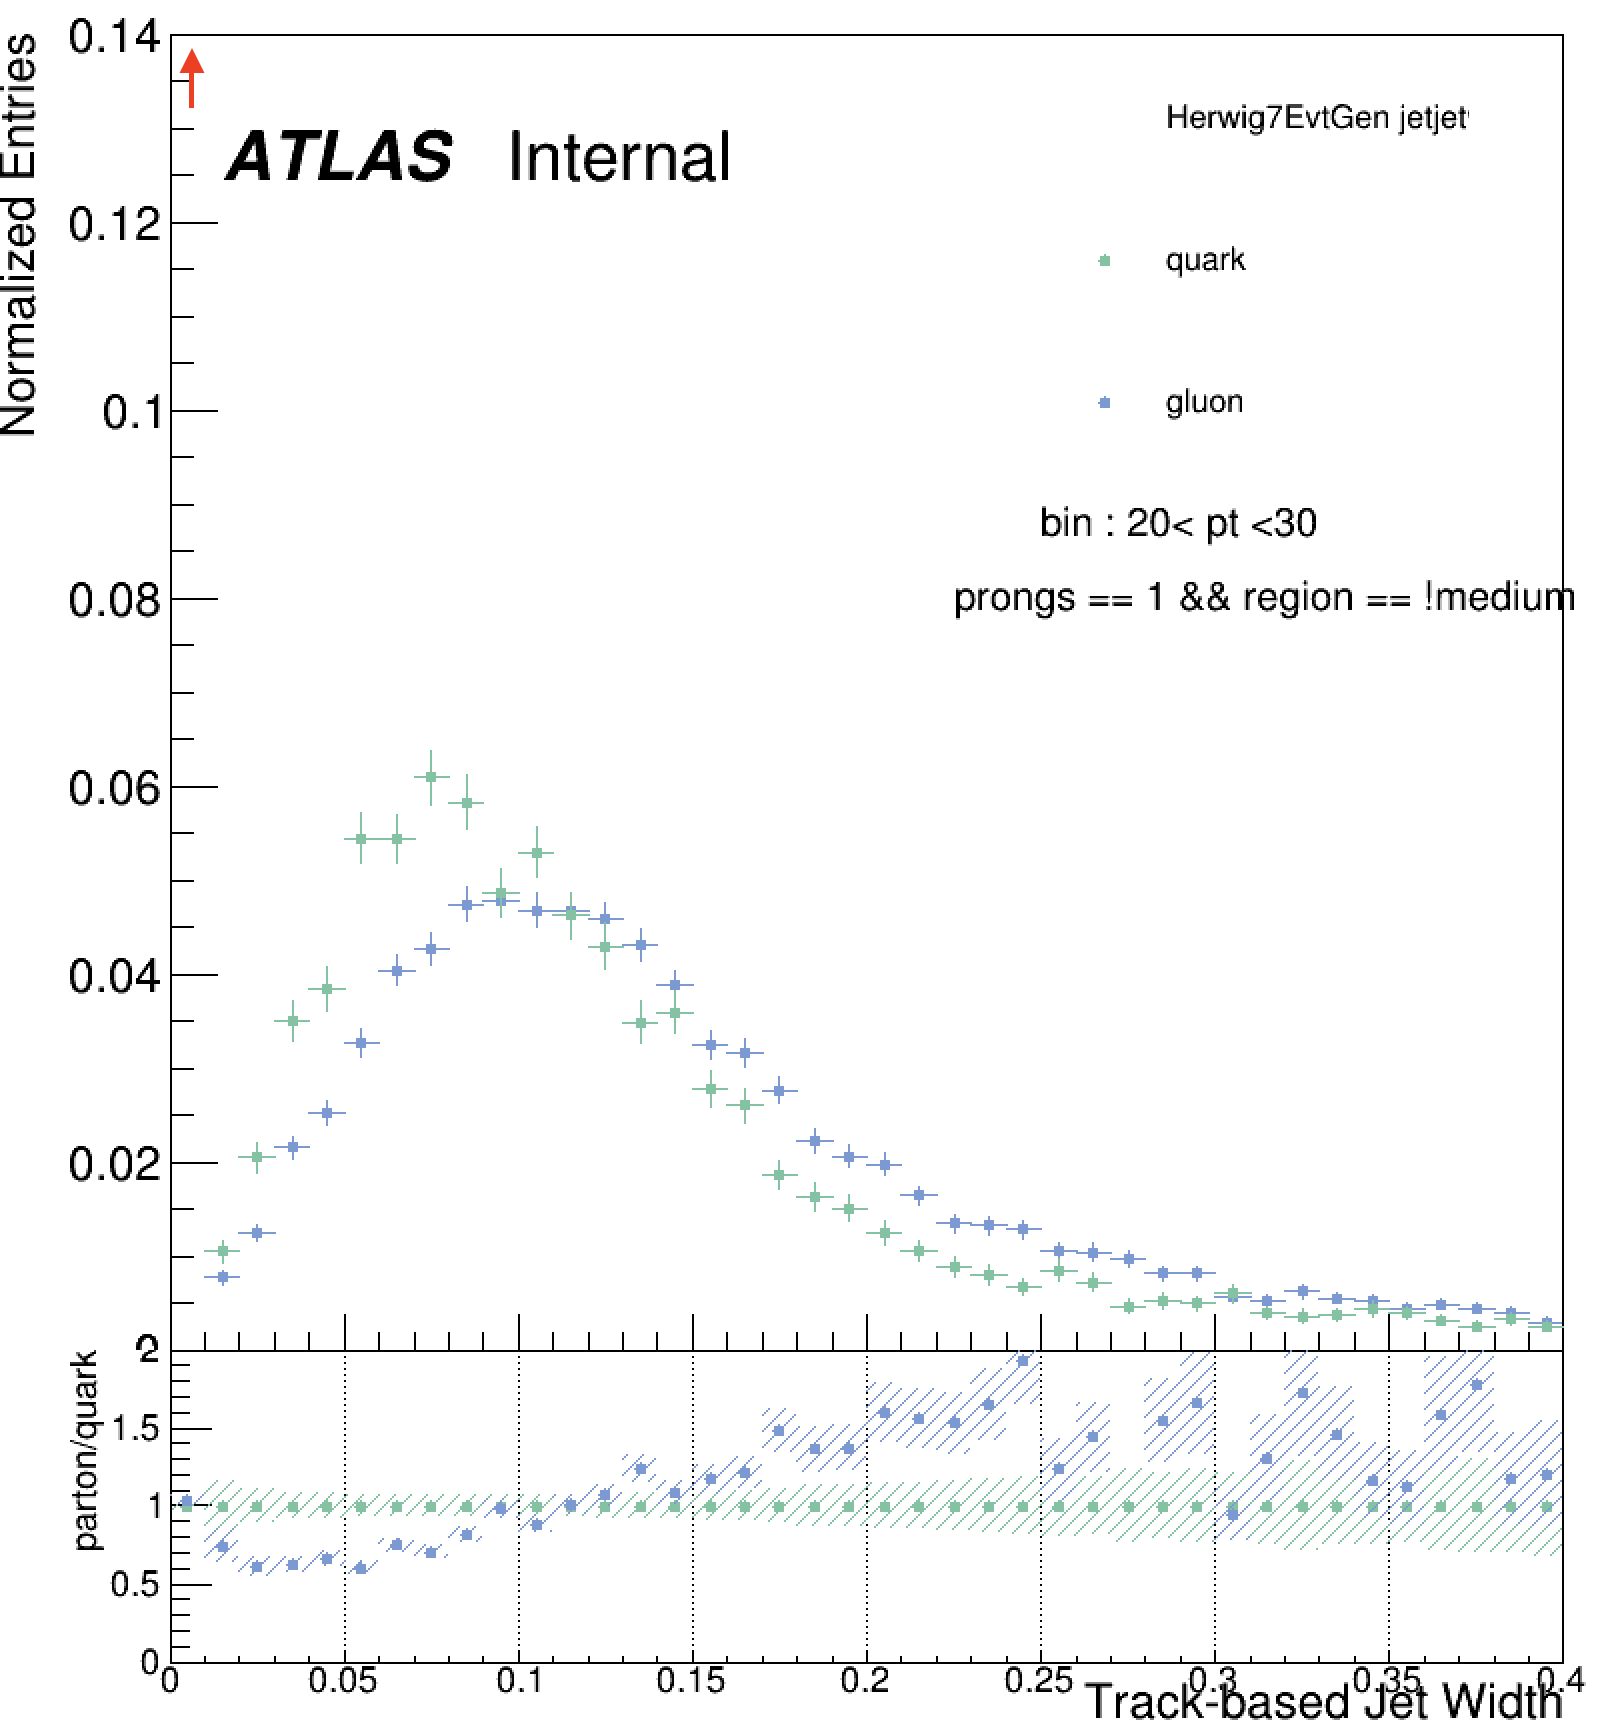
\includegraphics[width=0.4\textwidth]{FakeTau/Track_based_jet_width_Dijets}}\hspace{0.05\textwidth}
	\end{center}	
	\caption{Unit-normalised quark and gluon distributions of calo-based (top) and track-based (bottom) jet widths, in the \pt\ bin $[20,30]$ \gev, derived from \ac{MC} samples of Z+jets (left) and Dijet (right) events are shown in the top half of each plot. Underneath each template the ratio of parton to quarks (chosen as reference) is shown.  \htau\ candidates that fail the \textit{Medium} \ac{BDT} identification working point and have a minimum \ac{BDT} score of 0.005 are truth-matched to the corresponding parton. Red arrow indicate point that is outside the range of the graph.}
	\label{fig:jet_width_diff}
	\end{figure}	
	
	Some mis-modelling that is present in both the calo-based and track-based jet width is shown in Figure~\ref{fig:jet_width_modelling}. 
	The track-based (a) and calo-based (b) jet width are shown for the 1-prong visible \htau\ in a Z boson abundant region of phase space, derived using the following selection:
	\begin{itemize}
	%\item TAUP3 derivation samples
	\item A single muon trigger
	\item A leading muon \pt\ $>\,27$ GeV which is matched to the trigger
	\item The sub-leading muon  has \pt\ $>\,10$ GeV
	\item Two muons of opposite-sign charge that pass the \textit{Tight} isolation workingpoint\footnote{as defined in Reference~\cite{cite-key}}
	\item M($\mu,\mu$) $\in$ (81,101) GeV %$81 \,<\, \textrm{M}(\mu,\mu)\, <\, 101$ GeV 
	\item No electrons present 
	\item At least one visible \htau\ candidate with: %\pt\ $>\,20$ GeV,
	%\item At least one reconstructed tau with
	\begin{itemize}
		\item \pt\ $>\,20$ \gev
		\item Absolute charge of 1 
		\item 1 or 3 tracks associated with its vertex
		\item failed \textit{Medium} \ac{BDT} identification working point and no minimum score requirement
	\end{itemize}
	%\item The taus fail the Medium BDT identification working point and have no minimum score requirement
	\end{itemize}
	
	 The calo-based mis-modelling is caused by the mis-modeling of pileup jets in the sample which causes a different shape, as well as a shift, in the observed \ac{MC} calo-based jet width template compared to data. The track-based jet width template also shows some mis-modelling of the jet width. This is caused by the large number of jet width entries with values equal to -1, which cause the normalization to be off. For the 1-prong (\pt\ inclusive) visible \htau\ candidate a jet width value of -1 corresponds to $\approx30\%$ of the cases. Because ratio of data/MC for the track-based jet width in the bulk of the distribution is approximately flat, then the shape is well simulated albeit poorly normalized as mentioned previously. This allows for the track-based jet width to be used as discriminating variable for quark and gluon-initiated jets.
	 \begin{figure}[!hbt]
	\begin{center}
			 				\subbottom[]{
								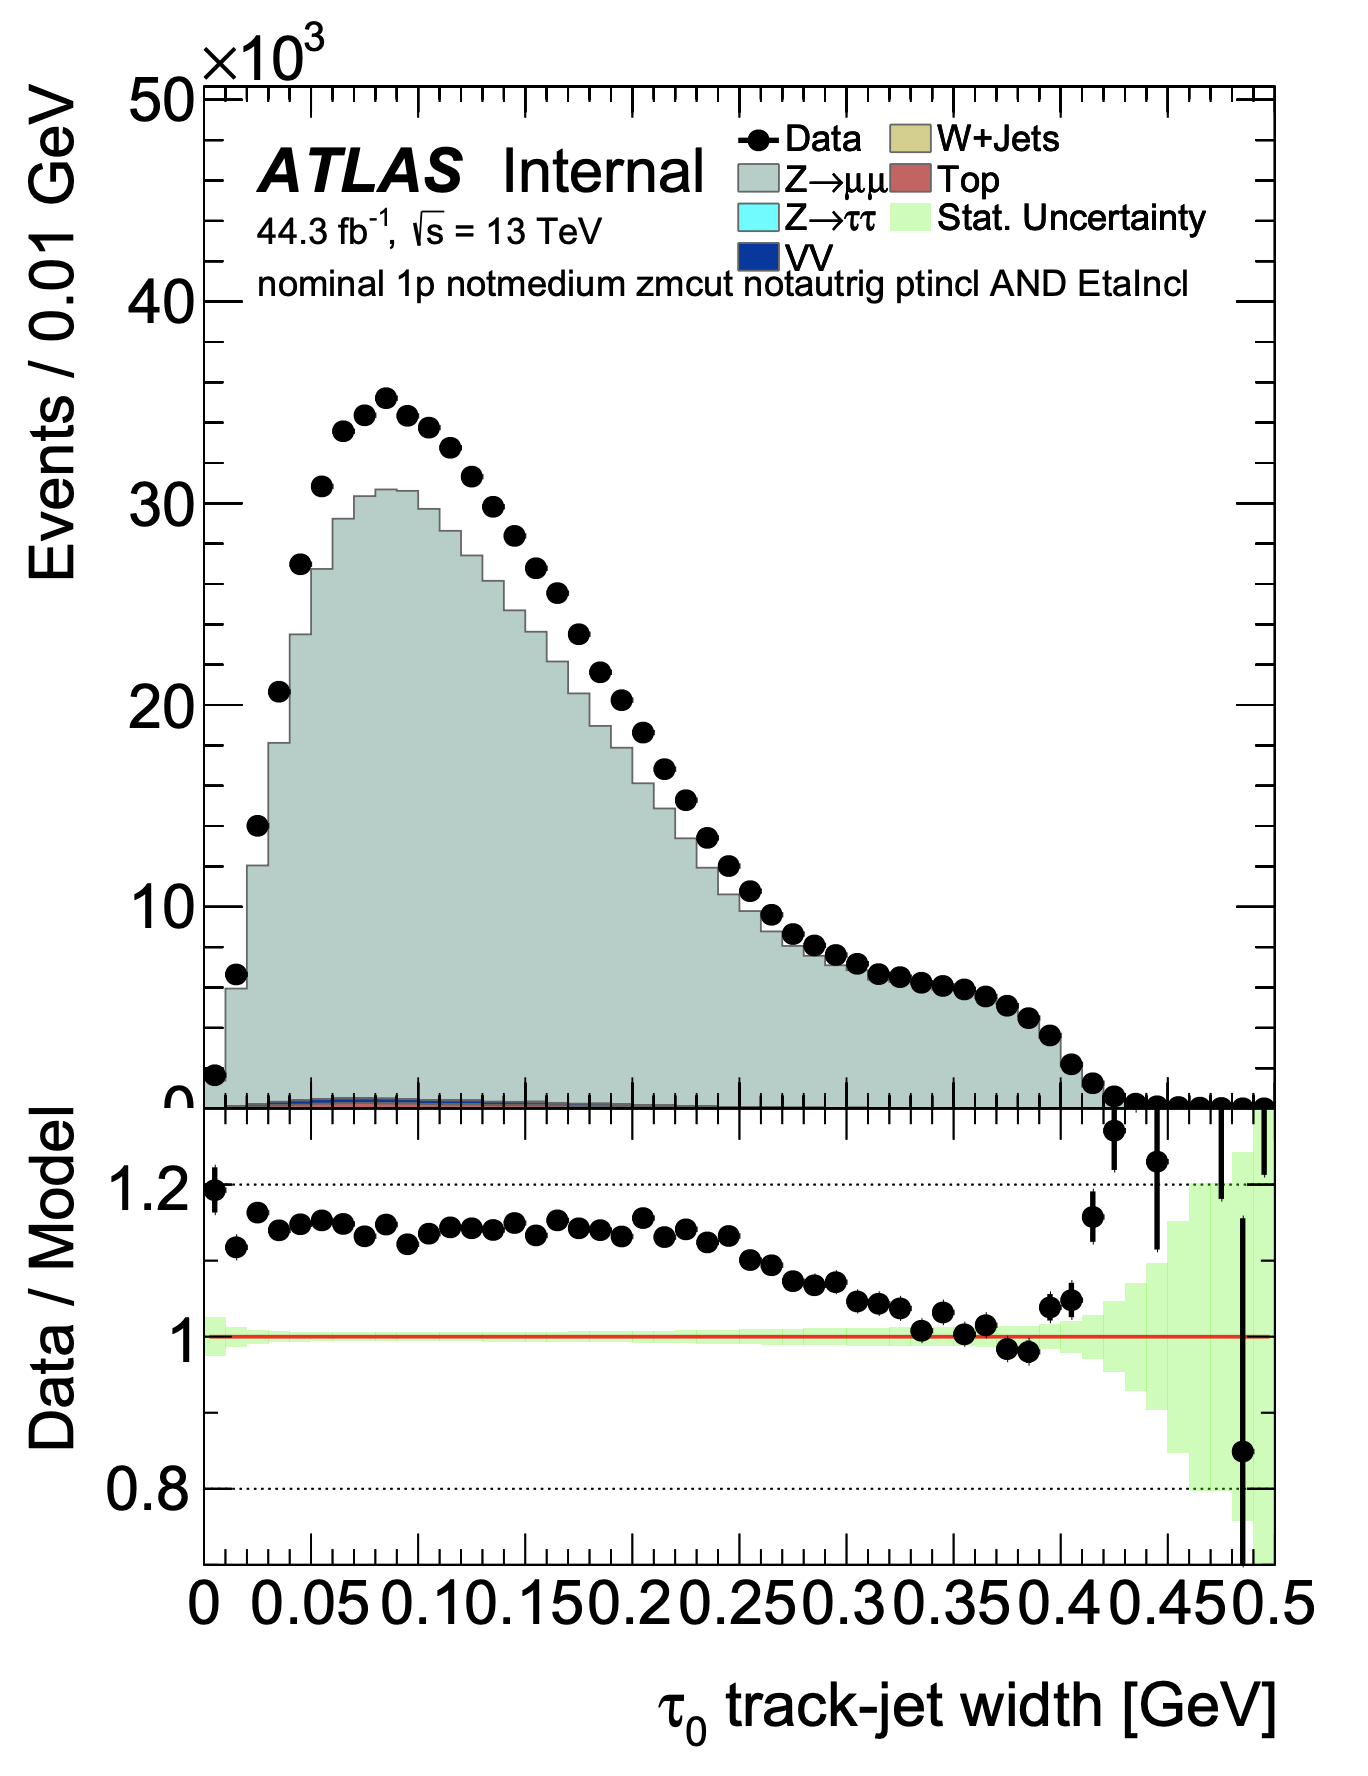
\includegraphics[width=0.45\textwidth]{FakeTau/track-based_jet_width_modelling}}\hspace{0.05\textwidth}
							\subbottom[]{
								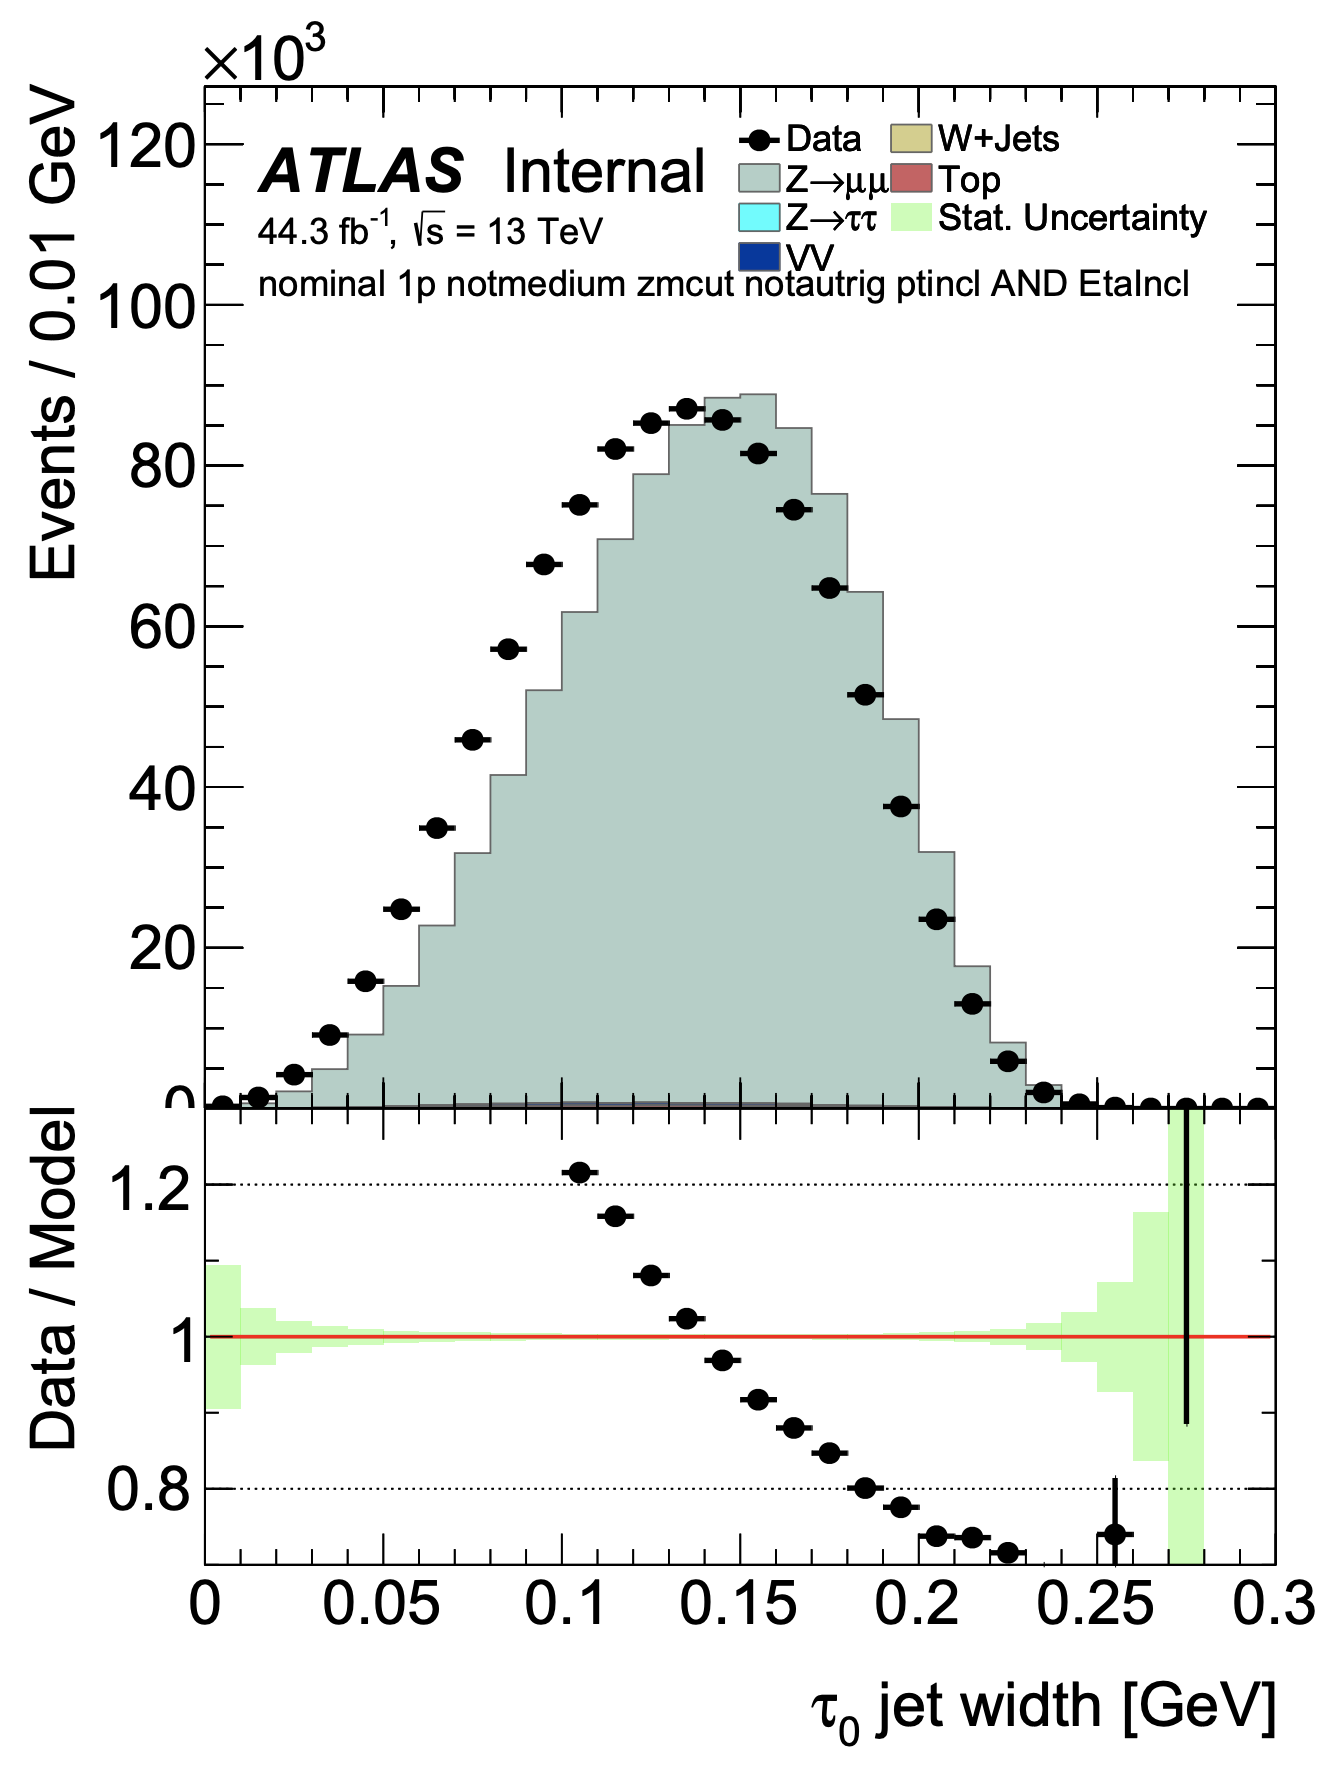
\includegraphics[width=0.45\textwidth]{FakeTau/calo-based_jet_width_modelling}}\hspace{0.05\textwidth}
	\end{center}	
	\caption{Distributions of visible \htau\ candidates jet width in Data and MC using a track-based (a) and calo-based (b) jet width. Top plots show the jet width distributions for different MC processes and 44.3 fb$^{-1}$ of collected data. Bottom plots show the Data/MC ratio, where 1 represents perfect agreement.}
	\label{fig:jet_width_modelling}
	\end{figure}
	
	
	
	\section{Data regions} 
	\label{sec:datareg}
	This section describes the two \ac{FF} regions used to derive FF$_1$ and FF$_2$ for interpolation, as described previously.
	The quark aboundant region is dominated by Z boson production in association with jets (\Zjets) with Z$\,\rightarrow\,\mu\mu$ events selected using a single $\mu$ trigger~\cite{CMS-PAS-JME-16-003}.
	The corresponding derived \ac{FF} values will be referred to as FF$_Z$ from here on.
	 The second region is a multi-jet gluon-enriched region, consisting of di-jet events triggered using a single jet trigger. The resulting \ac{FF} value corresponding to this region will be referred to as FF$_{MJ}$.
	 
	% \color{red} Show that Z+jets are quark dominated and di-jet samples are gluon dominated (to be added perhaps to Appendix A)\color{black}
	 
	\subsection{Quark abundant region}\label{subsec:quarkregion}	
	The \Zjets\ region was isolated in data using the following selection:
	\begin{itemize}
	%\item TAUP3 derivation samples
%	\item Trigger given in Appendix ~\ref{app:FTTF_Zjets_data_trigs}
	\item Event are accepted if any of the the following single muon triggers are fired: 
		\begin{itemize}
		\item For data collected in 2015:
			\begin{itemize}
				\item HLT\_mu20\_iloose\_L1MU15
				\item HLT\_mu50
			\end{itemize}
		\item For data collected in 2016 onwards:
			\begin{itemize}
				\item HLT\_mu26\_ivarmedium
				\item HLT\_mu50
			\end{itemize}
		\end{itemize}
	%\item No electrons identified with the loose \ac{LH} based identification criteria described in References ~\cite{ele_id,Aad_2019} and with \pt\ $>\,15$ GeV
	\item No electrons that pass the \textit{Loose} identification criteria\footnote{\ac{LH} based electron identification criteria is described in detail in References~\cite{ele_id,Aad_2019}} and with \pt\ $>\,15$ GeV
	\item Exactly two reconstructed muons with
	\begin{itemize}
		\item Muon passes the \textit{Tight} track-based isolation working point~\cite{cite-key}
		\item Leading \pt\ $>\,27.3$ GeV and matched to trigger
		\item Sub-leading \pt $>\,10.0$ GeV 
		\item \textit{Medium} quality~\cite{cite-key}
		\item $M(\mu,\mu)\,\in$ (70,100) GeV
	\end{itemize}
	\item Exactly one reconstructed tau with
	\begin{itemize}
		\item \pt\ $>\,18.0$ GeV
		\item Absolute charge of 1 
		\item 1 or 3 tracks associated with its vertex
		\item \ac{RNN} efficiency score $>$ 0.01
	\end{itemize}
	\end{itemize}
	
	Using the above selection a region predominately dominated by \Zjets\,, that is abundant with quark-initiated tau-faking jets, is obtained. 
	Using the method described in Section~\ref{sec:ffmeth} the values for the FFs can thus be derived for any given region or anti-region of identification working point. 
	
	\begin{figure}[!htb]
	\begin{center}
			 				\subbottom[]{
								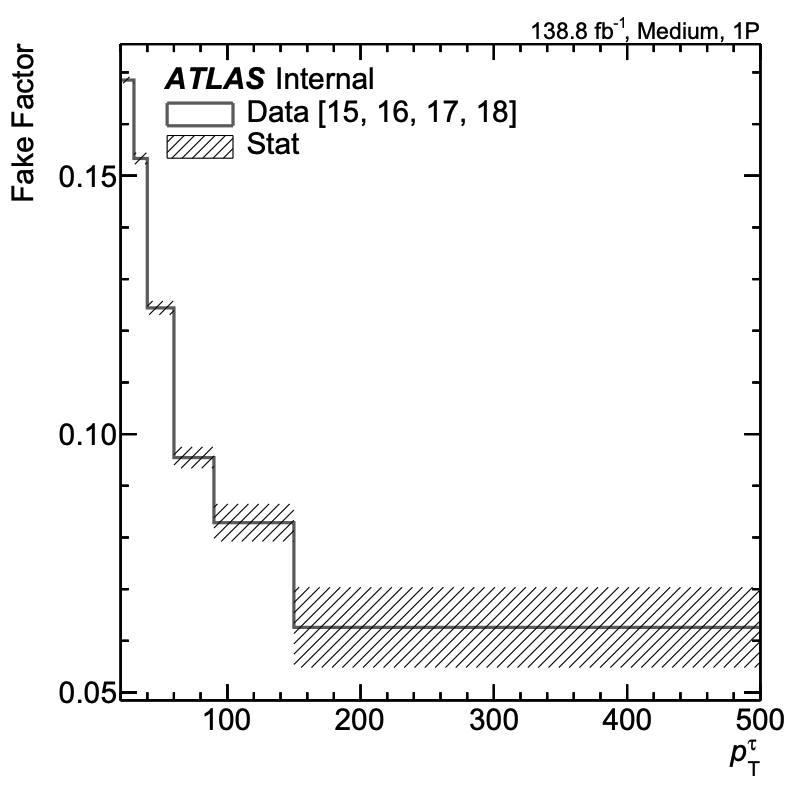
\includegraphics[width=0.45\textwidth]{FakeTau/Zjets_1p_FF}}\hspace{0.05\textwidth}
							\subbottom[]{
								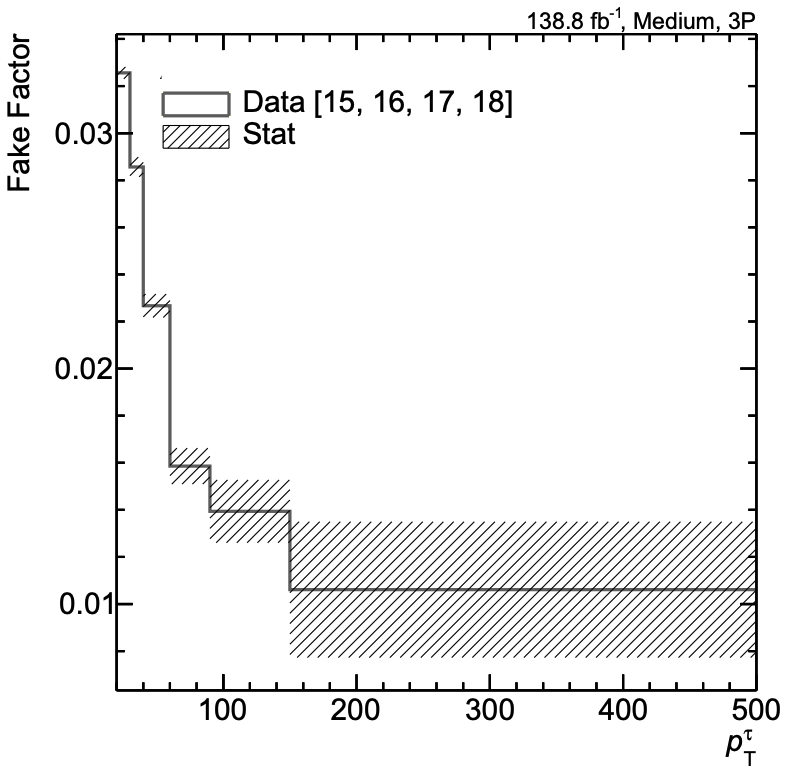
\includegraphics[width=0.45\textwidth]{FakeTau/Zjets_3p_FF}}\hspace{0.05\textwidth}
	\end{center}
	\caption{Distributions of FF values as a function of the leading visible \htau\ object in the Z+jets quark-initiated tau-faking-jets abundant data region for the one prong (left) and three prong (right) case using \textit{Medium} \ac{RNN} working point and full Run-2 data.(From [Petar slides])}
	\label{fig:Zjets_data_FF}
	\end{figure}
	Figure~\ref{fig:Zjets_data_FF} shows the visible \htau\ \ac{FF} values with respect to the leading tau \pt\ (denoted by $p_T^{\tau}$ in the figure) derived from data using the selection above. Real $\tau$ are subtracted using \ac{MC} simulations, for a \textit{Medium} \ac{RNN} working point for 1 prong (a) and 3 prong (b) case, as defined by equation~\ref{eq:FF1}. The FF values show a strong dependence with \pt, where the FF value decreases as the visible \htau object \pt\ increases, as well as lower value for the FF of the 3 pronged tau. 	

As discussed in Section~\ref{sec:faketau}, the rejection power of both \ac{RNN} and \ac{BDT} classifiers increases with increasing \pt. In a \ftau\ dominated sample, as the \pt\ increases there the chance for the classifier to identify and reject \ftau also increases. This will in turn decrease the number of \htau\ objects that populate the pass-ID region (nominator of equation~\ref{eq:FF1}), whilst simultaneously increasing the fail-ID region (denominator of equation~\ref{eq:FF1}). The \ac{FF} as a function of \htau\ \pt\ in region that is abundant in \ftau candidates, such as the one described above, is thus expected to decrease with increasing \pt.

 %as the pt increases the fake tau rejection power for both RNN and BDT classifiers increase. This will decrease the number of taus that populate the ID region for the higher pts (since there is better fake rejection) whist instead increasing multiplicity for the anti-id region.
 
%	As explained in Section ~\ref{sec:faketau} the reconstruction efficiency decreases with increasing \htau\ \pt due to the higher probability of wrongly classifying an electron from photon conversion as a charged hadron and for higher energy \htau\ to fail the number of pixel hits requirement.
%	Because of this as the \htau\ \pt\ increases the population of  relatively higher number of mis-reconstructed taus in the high \pt\ bins compared to the lower, at any identification working point. 
%	The trend of decreasing FF values with increasing \pt\ seen in figure ~\ref{fig:Zjets_data_FF} is therefore explained since, as the \pt\ increases the denominator of equation ~\ref{eq:FF1} will become larger, which in turn will result in the decreasing values of FF.
	
	%The dependence on \pt\ of the FF values is due to the dependence of reconstruction efficiency with \pt, which decreases with increasing \pt\ as explained in section ~\ref{sec:faketau}. The classifier will therefore have a relatively higher number of mis-reconstructed taus in the high \pt\ bins compared to the lower, which will result into a larger number of fake \htau rejected for the given working point. The denominator of equation ~\ref{eq:FF1} will thus be larger in the higher \pt\ bins which results in lower FF values. 
	The lower FF values of the 3 prong tau case compared to the 1 prong, are due to the higher rejection power of the \ac{RNN}/\ac{BDT} classifier for the 3 prong taus. This results in a relatively higher multiplicity of taus which fail the identification working point compared to the 1 prong scenario. 
	
	\subsection{Gluon abundant region}\label{subsec:gluonregion}
	The Multi-jet production was isolated in data to derive a gluon abundant region to derive FF values as in ~\ref{subsec:quarkregion}. To achieve this the following selection was used:
	\begin{itemize}
	%\item TAUP3 derivation samples
	%\item Trigger given in Appendix ~\ref{app:FTTF_Dijets_data_trigs}
	\item Event are accepted if any of the the following single jet triggers are fired: 
	\begin{itemize}
		\item HLT\_j15 with offline $\pt\,>\,20$ GeV
		\item HLT\_j25 with offline $\pt\,>\,35$ GeV
		\item HLT\_j35 with offline $\pt\,>\,45$ GeV
		\item HLT\_j85 with offline $\pt\,>\,110$ GeV
		\item HLT\_j110 with offline $\pt\,>\,120$ GeV
		\item HLT\_j175 with offline $\pt\,>\,216$ GeV
		\item HLT\_j260 with offline $\pt\,>\,300$ GeV
		\item HLT\_j360 with offline $\pt\,>\,400$ GeV
		\item HLT\_j400 with offline $\pt\,>\,440$ GeV
		\item HLT\_j420 with offline $\pt\,>\,460$ GeV
	\end{itemize}
	\item  No electrons that pass \textit{Loose} identification criteria\footnote{\ac{LH} based electron identification criteria is described in detail in References~\cite{ele_id,Aad_2019}} with \pt\ $>\,15$ GeV
	\item No \textit{Loose} quality muon with \pt\ $>\,7$ GeV
	\item No photon that passes the \textit{Loose} identification criteria~\cite{ele_id,Aad_2019} with \pt\ $>\,10$ GeV 
	\item At least one jet
	\begin{itemize}
	\item \pt\ $>\,20$ GeV
	\item $\eta\,<4.5$
	\item No \ac{JVT}\footnote{The \ac{JVT} is a multivariate combination of track-based variables used to suppress pileup jets~\cite{ATLAS-CONF-2014-018}} requirement 
	\end{itemize}
	\item Loose jet cleaning
	\item \ac{OR}\footnote{\ac{OR} procedure discussed in detail in Section~\ref{sec:ORprocedure}} procedure is performed
	\begin{itemize}
	\item With loosely selected electrons, muons, taus, photons, and jets
	\item Where tau selection before \ac{OR}: \pt\ $>\,20$ \gev, \ac{RNN} $>\,0.01$ 
	\end{itemize}
	\end{itemize}
	\begin{figure}[!htb]
	\begin{center}
			 				\subbottom[]{
								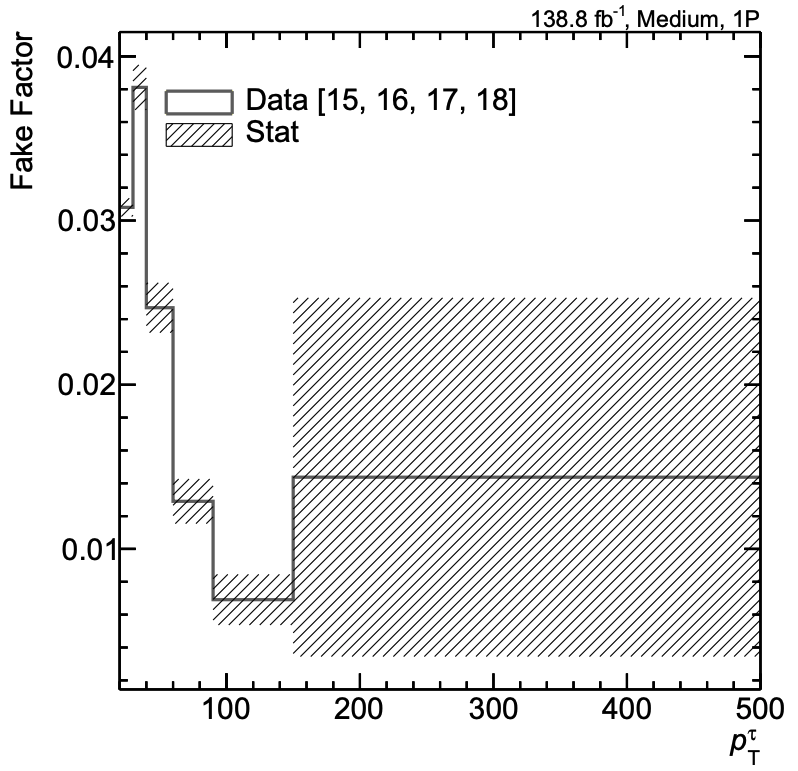
\includegraphics[width=0.45\textwidth]{FakeTau/Dijets_1p_FF}}\hspace{0.05\textwidth}
							\subbottom[]{
								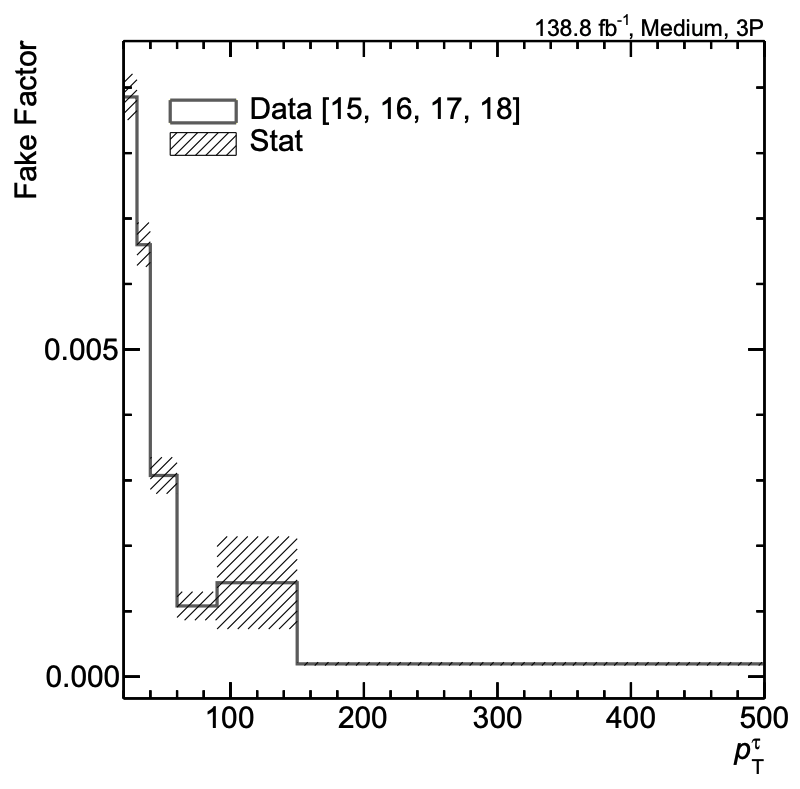
\includegraphics[width=0.45\textwidth]{FakeTau/Dijets_3p_FF}}\hspace{0.05\textwidth}
	\end{center}
	\caption{Distributions of FF values as a function of the leading visible \htau\ object in the di-jets gluon-initiated tau-faking-jets abundant data region for the one prong (left) and three prong (right) case using "Medium RNN" working point and full Run-2 data. Truth tau subtraction has not been applied to these results. (From [Petar slides])}
	\label{fig:Dijets_data_FF}
	\end{figure}
	Figure~\ref{fig:Dijets_data_FF} shows the FF values derived for this region for the 1 prong (a) and 3 prong (b) cases, as a function of the leading visible \htau\ \pt\ for the \textit{Medium} RNN working point. The FF values are found to be dependent on the leading \htau\ \pt, similarly to the Z+jets region, but with slightly lower values. 
	This is due to the high multiplicity of jets in this region which have a higher probability of being mis-identified as taus. This results in a larger multiplicity of taus failing the RNN working point, thus translating to lower FF values.
	 It is worth noting that the large uncertainty band shown in the highest \pt bin for both 1 case is due to low statistics in that bin from the 2017 collected data. 
	
	\section{MC Inputs}
	\label{sec:mcinputs}
	In this section the \ac{MC} samples, generators, selections, and required calibrations used to produce the track based jet width and \ac{FF} distributions required to determine the quark fraction needed for the estimation of the \ac{FF} values are discussed.
	Section~\ref{sec:uniffmeth}  describes how through the derivation of pure quark and pure gluon track based jet width templates it is possible  to calculate the relative abundance of quarks (quark fraction) in a given sample using a fitting procedure (will be discussed in more detail in Section~\ref{sec:TFFT}). 
	The track based jet width, and \htau\ transverse momentum distributions derived from \ac{MC} samples used for the quark fraction fitting will be referred as templates from here on.
	
	\subsection{Samples and generators}
	\label{subsec:FTTFsample}
	Parton kinematics can differ slightly depending on the generator used due to the different methods and prescriptions used for the Matrix Element-Parton shower matching. To account for this systematic effect different MC samples, generated using different generators, have been studied. 
	The samples studied are separated into two categories: \ac{HP} and \ac{LP} samples. 
	\ac{HP} samples include only Z+jets, W+jets and di-jets processes that have been produced by similar generator and with significant statistics. \ac{LP} samples include a wider range of processes produced with different generators, and can be used to study the generator effects and boost  the overall statistics. 
	
	The \ac{HP}
	%\footnote{Full list of HP samples can be found in appendix ~\ref{app:HPsamples}}
	% that have been studied at Analysis Object Data (AOD) level (i.e. the MC samples have been gone through the generation, simulation, digitization and reconstruction processes but havent gone through any derivation) 
	 \Zjets\ and \Wjets\ samples have been generated using \textsc{Powheg-Box} v1~\cite{powheg} interfaced to the \textsc{Pythia v8.186}~\cite{pythia8}( referred as \textsc{Pythia 8} from now on) \ac{PS} and hadronisation model, except for the heavy-flavour decays which are modelled using the \textsc{EvtGen v1.2.0}~\cite{evtgen} program. The \textsc{CTEQ6L1} \ac{PDF}~\cite{cteq6l1} is used for the parton shower along with the \textsc{AZNLO}~\cite{aznlo} set of tuned parameters.
	%There is also a set of di-jet samples that are part of the \ac{HP} list of samples. 
	The \ac{HP} di-jet samples are generated using the \textsc{Pyhtia 8} and \textsc{EvtGen} combination as above, but using the \textsc{A14} set~\cite{ATL-PHYS-PUB-2014-021} of tune parameters with the \textsc{NNPDF2.3 LO} PDF~\cite{BALL2013244} set instead and are separated into several slices of different generator-level jet \pt\ thresholds, generally referred to as "JZx" (with x running from 0 to the number of slices)~\cite{Marshall:2016630}. 
	JZxW is the same as JZx slicing but filtered based on the \pt\ spectrum such that there are equal numbers of events at each \pt.   

\begin{table}[!hbt]
	\caption{Sample and generators used for \ac{FF} studies. Generators for each samples are shown with corresponding \ac{PDF} sets, selections and filters. Sample names shown in bold text represent \ac{HP} samples, rest are considered \ac{LP} samples.}
	%\documentclass[10pt]{article}
%\usepackage[usenames]{color} %used for font color
%\usepackage{amssymb} %maths
%\usepackage{amsmath} %maths
%\usepackage[utf8]{inputenc} %useful to type directly diacritic characters
%\usepackage{multirow}
%\usepackage{graphicx}\begin{document}
% Please add the following required packages to your document preamble:
% \usepackage{multirow}
%\begin{table}[!hbt]
\resizebox{\textwidth}{!}{\begin{tabular}{ccccc} \hline 
Processes & Generators & PDF & veto / filter & selection / comments \\ \hline \hline
\multirow{5}{*}{\begin{tabular}[c]{@{}c@{}}\\ \\ \\ \\ \\ \textbf{Z+jets}\\ \textbf{W+jets}\end{tabular}} & \multirow{3}{*}{\textsc{Sherpa v2.2.1}} & \multirow{3}{*}{\textsc{NNPDF3.0 NNLO}} & \begin{tabular}[c]{@{}c@{}}c-jet veto and b-jet veto \\ OR \\ c-jet filter and b-jet veto \\ OR \\ b-jet filter\end{tabular} & \begin{tabular}[c]{@{}c@{}}$m(\ell,\ell)\,>\,40$ GeV\\  $\textrm{max}(\textrm{HT},p_T^V)\,\in\,[0,70,140,280,500,1000,\textrm{inf}]$\end{tabular} \\ \cline{4-5} 
 &  &  & b-jet veto OR b-jet filter & \begin{tabular}[c]{@{}c@{}}10 GeV $<\,m(\ell,\ell)\,<\,$ 40 GeV,\\ $\textrm{max}(\textrm{HT},p_T^V)\,\in\,[0,70,140,280,\textrm{inf}]$\end{tabular} \\ \cline{2-5} 
 & \multirow{2}{*}{\begin{tabular}[c]{@{}c@{}}\textsc{MadGraph5\_aMC@NLO v2.2.3.p4} \\                              + \textsc{Pythia 8} + \textsc{EvtGen v1.2.0}\end{tabular}} & \begin{tabular}[c]{@{}c@{}}\textsc{A14}\\ \textsc{NNPDF2.3 LO}\end{tabular} & \begin{tabular}[c]{@{}c@{}}c-jet veto and b-jet veto\\ OR\\ c-jet filter and b-jet veto\\ OR\\ b-jet filter\end{tabular} & \begin{tabular}[c]{@{}c@{}}$m(\ell,\ell)\,>40$ GeV\\  $\textrm{HT}\,\in\,[0,70,140,280,500,1000,2000,\textrm{inf}]$\end{tabular} \\ \cline{4-5} 
 &  &  & \multicolumn{1}{l}{} & $N_p\,\in\,[0,1,2,3,4]$ (*only for some $Z\rightarrow\tau\tau$ samples) \\ \cline{2-5} 
 & \textbf{ \textsc{Powheg v1} + \textsc{Pythia 8} + \textsc{EvtGen v1.2.0}} & \begin{tabular}[c]{@{}c@{}}\textbf{\textsc{AZNLO}}\\ \textbf{\textsc {CTEQ6L1}}\end{tabular} &  & $m(\ell,\ell) > 60$ GeV \\ \hline \hline
\multirow{4}{*}{\begin{tabular}[c]{@{}c@{}}\\ \\ \\ \\ Multiboson\end{tabular}} & \begin{tabular}[c]{@{}c@{}}\\ \\ \textsc{Sherpa v2.2.1}\end{tabular} & \multirow{3}{*}{\begin{tabular}[c]{@{}c@{}}\\  \\ \\ \textsc{NNPDF3.0 NNLO}\end{tabular}} &  & on shell diboson production with factorised decays \\ \cline{2-2} \cline{4-5} 
 & \multirow{2}{*}{\begin{tabular}[c]{@{}c@{}}\\ \\ \textsc{Sherpa v2.2.2}\end{tabular}} &  & \multirow{2}{*}{} & \begin{tabular}[c]{@{}c@{}}$m(\ell,\ell)_{SFOS} \,>\, 4$ GeV\\  $p_T(\ell_1)\,>\,5$ GeV\\  $p_T(\ell_2)\,>\,5$ GeV\end{tabular} \\ \cline{5-5} 
 &  &  &  & \begin{tabular}[c]{@{}c@{}}$m(\ell,\ell)\,>\,2\times m_{\ell}+250$ MeV\\ ($p_T(\ell_1)\,>\,20$ GeV OR $p_T(\ell_2)\,>\,50$ GeV)\\ AND\\ ($p_T(\ell_2)\,<\,5$ GeV OR $m(\ell_{SFOS == 1})\,<\,4$ GeV)\end{tabular} \\ \cline{2-5} 
 & \textsc{Powheg v2} + \textsc{Pythia 8} + \textsc{EvtGen v1.2.0} & \begin{tabular}[c]{@{}c@{}}\textsc{AZNLO}\\ \textsc{CTEQ6L1}\end{tabular} & \multicolumn{1}{l}{} & $m(\ell,\ell)_{min}\,>\,4$ GeV \\ \hline \hline
\multirow{4}{*}{\textbf{Dijets}} & \multirow{1}{*}{Herwig v7.0.4 + EvtGen v1.6.0} & \begin{tabular}[c]{@{}c@{}}\textsc{NNPDF3.0 NLO} (ME)\\\textsc{MMHT2014} (shower/MPI)\end{tabular} &  & JZx with x $\in[1,2,3,4,5,6,7,8,9,10,11]$ \\ \cline{2-3} \cline{5-5} \\
 & \textbf{\textsc{Pythia 8} + \textsc{EvtGen v1.2.0}}  & \begin{tabular}[c]{@{}c@{}}\textbf{\textsc{A14}}\\ \textbf{\textsc{NNPDF23LO}}\end{tabular} & & JZxW with x $\in[1,2,3,4,5,6,7,8,9,10,11,12]$ \\ \hline \hline
\multirow{9}{*}{single top + $t\bar{t}$} & \multirow{4}{*}{\textsc{Powheg} + \textsc{Pythia 8} + \textsc{EvtGen v1.6.0}} & \multirow{4}{*}{\begin{tabular}[c]{@{}c@{}}\textsc{A14}\\ \textsc{NNPDF23LO}\end{tabular}} & non-hadronic decays & \multirow{2}{*}{$h_{damp}\,=\,258.75$ GeV (1.5 $\times$ top mass)} \\ \cline{4-4}
 &  &  & hadronic decays &  \\ \cline{4-5} 
 &  &  & inclusive & \multicolumn{1}{l}{} \\ \cline{4-4}
 &  &  & leptonic decay & \multicolumn{1}{l}{} \\ \cline{2-5} 
 & \multirow{5}{*}{\textsc{Powheg} + \textsc{Herwig v7.0.4} + \textsc{EvtGen v1.6.0}} & \multirow{5}{*}{\begin{tabular}[c]{@{}c@{}}\textsc{NNPDF3.0 NLO} (ME)\\ \textsc{MMHT2014} (shower/MPI)\end{tabular}} & single lepton & \multirow{3}{*}{$h_{damp}\,=\,258.75$ GeV (1.5 $\times$ top mass)} \\ \cline{4-4}
 &  &  & di-lepton &  \\ \cline{4-4}
 &  &  & all hadronic &  \\ \cline{4-5} 
 &  &  & leptonic decay & \multicolumn{1}{l}{} \\ \cline{4-4}
 &  &  & inclusive & \multicolumn{1}{l}{} \\ \hline 
\end{tabular}}
%\end{table}
%
%\end{document}	
	\label{tab:LPsample}
	\end{table}	
	Table~\ref{tab:LPsample} summarises the samples and generators as well as any filtering or slicing that were applied to each sets of samples.
As mentioned previously, \ac{HP} samples are used as the main samples for comparison, while \ac{LP} samples have been used for further studies of generator and process driven effects.
	%\subsection{Template and Fake Factor Universality}
	\subsection{Analysis Object Data Samples selection}
	\label{subsec:AODsel}
	%\label{subsec:FFuniv}	
	%\subsubsection*{MC selections}
	\ac{AOD} samples are the baseline \ac{MC} samples produced by the \ac{ATLAS} collaboration. \ac{AOD} samples are not skimmed or slimmed for any particular type of analysis and instead are composed of the full collections of reconstructed objects. This makes these type of samples very useful to use for an initial proof of concept as the samples wont be affected by any bias introduced by any applied selections, calibrations or derivations. 
	To maintain the unbiased property of the \ac{AOD} samples only a very loose selection is used to select a region abundant with fake \htau\ objects.
	%For the \ac{MC} templates the required selections are much looser compared to the ones applied to data. 
	%It is important to main the high abundance of quarks (or gluons depending of the sample) already present in these samples and not bias the jet-faking \htau\ via selections. 
	 The following selection cuts are thus applied: 
	\begin{itemize}
	\item At least one tau:
		\begin{itemize}
		\item \pt\ $>$ 20 \gev
		\item \ac{BDT} background rejection efficiency score $>$ 0.005 
		\end{itemize}
	\end{itemize}
	Where the \ac{BDT} was later changed to the better performing \ac{RNN} identifier, following the recommendations for the appropriate reconstruction of the visible \htau, and thus changing the \ac{BDT} score  selection to RNN background rejection efficiency score > 0.01.
	%The lower \pt threshold is set at a level to achieve 95\% identification efficiency, and with BDT idenfitication score above 0.005 to reject any pileup jets.
	The \htau\ are categorised accoring to their \ac{PDG ID}s~\cite{PDG} from the results of the truth  matching procedure.
	%and is defined im the samples by the preperty \textsc{ConeTruthLabelID}
	To truth match the visible \htau\ to their corresponding \htau -faking parton, the jet seeding the \htau\ object is identified and is used for the truth-matching.
	% This is described in the code by the \textsc{PartonTruthLabelID}.
	Table~\ref{tab:pdg_match} shows the categories used to describe the truth-matched visible \htau\ objects using the variables: \textsc{ConeTruthLabelID} for identifying the \htau\ faking jets and \textsc{PartonTruthLabelID} to identify \htau candidates truth-matched to parton jets. 
	Both variables use the absolute value of \ac{PDG ID} values to describe the appropriate truth-matched object. 
	\begin{table}[!hbt]
	\caption{Truth table for selection of quark, gluon and un-matched candidates from jet-faking \htau objects identified via the truth matching method.}
	\begin{center}
	\input{tables/PDG_match}
	\end{center}
	\label{tab:pdg_match}
	\end{table}
	
	% It is important to note that \textsc{ConeTruthLabelID} can have both positive and negative values when identifying particles and anti-particles respectively. Whereas the \textsc{PartonTruthLabelID} can only have: positive values of PDG ID when the matching is successful, a value of 0 if no truth seed jet is found for that object and a value of -1 if  no parton if found to be truth-matched to the seeding jet. 
	\begin{figure}[!hbt]
		\begin{center}
			\subbottom[]{
				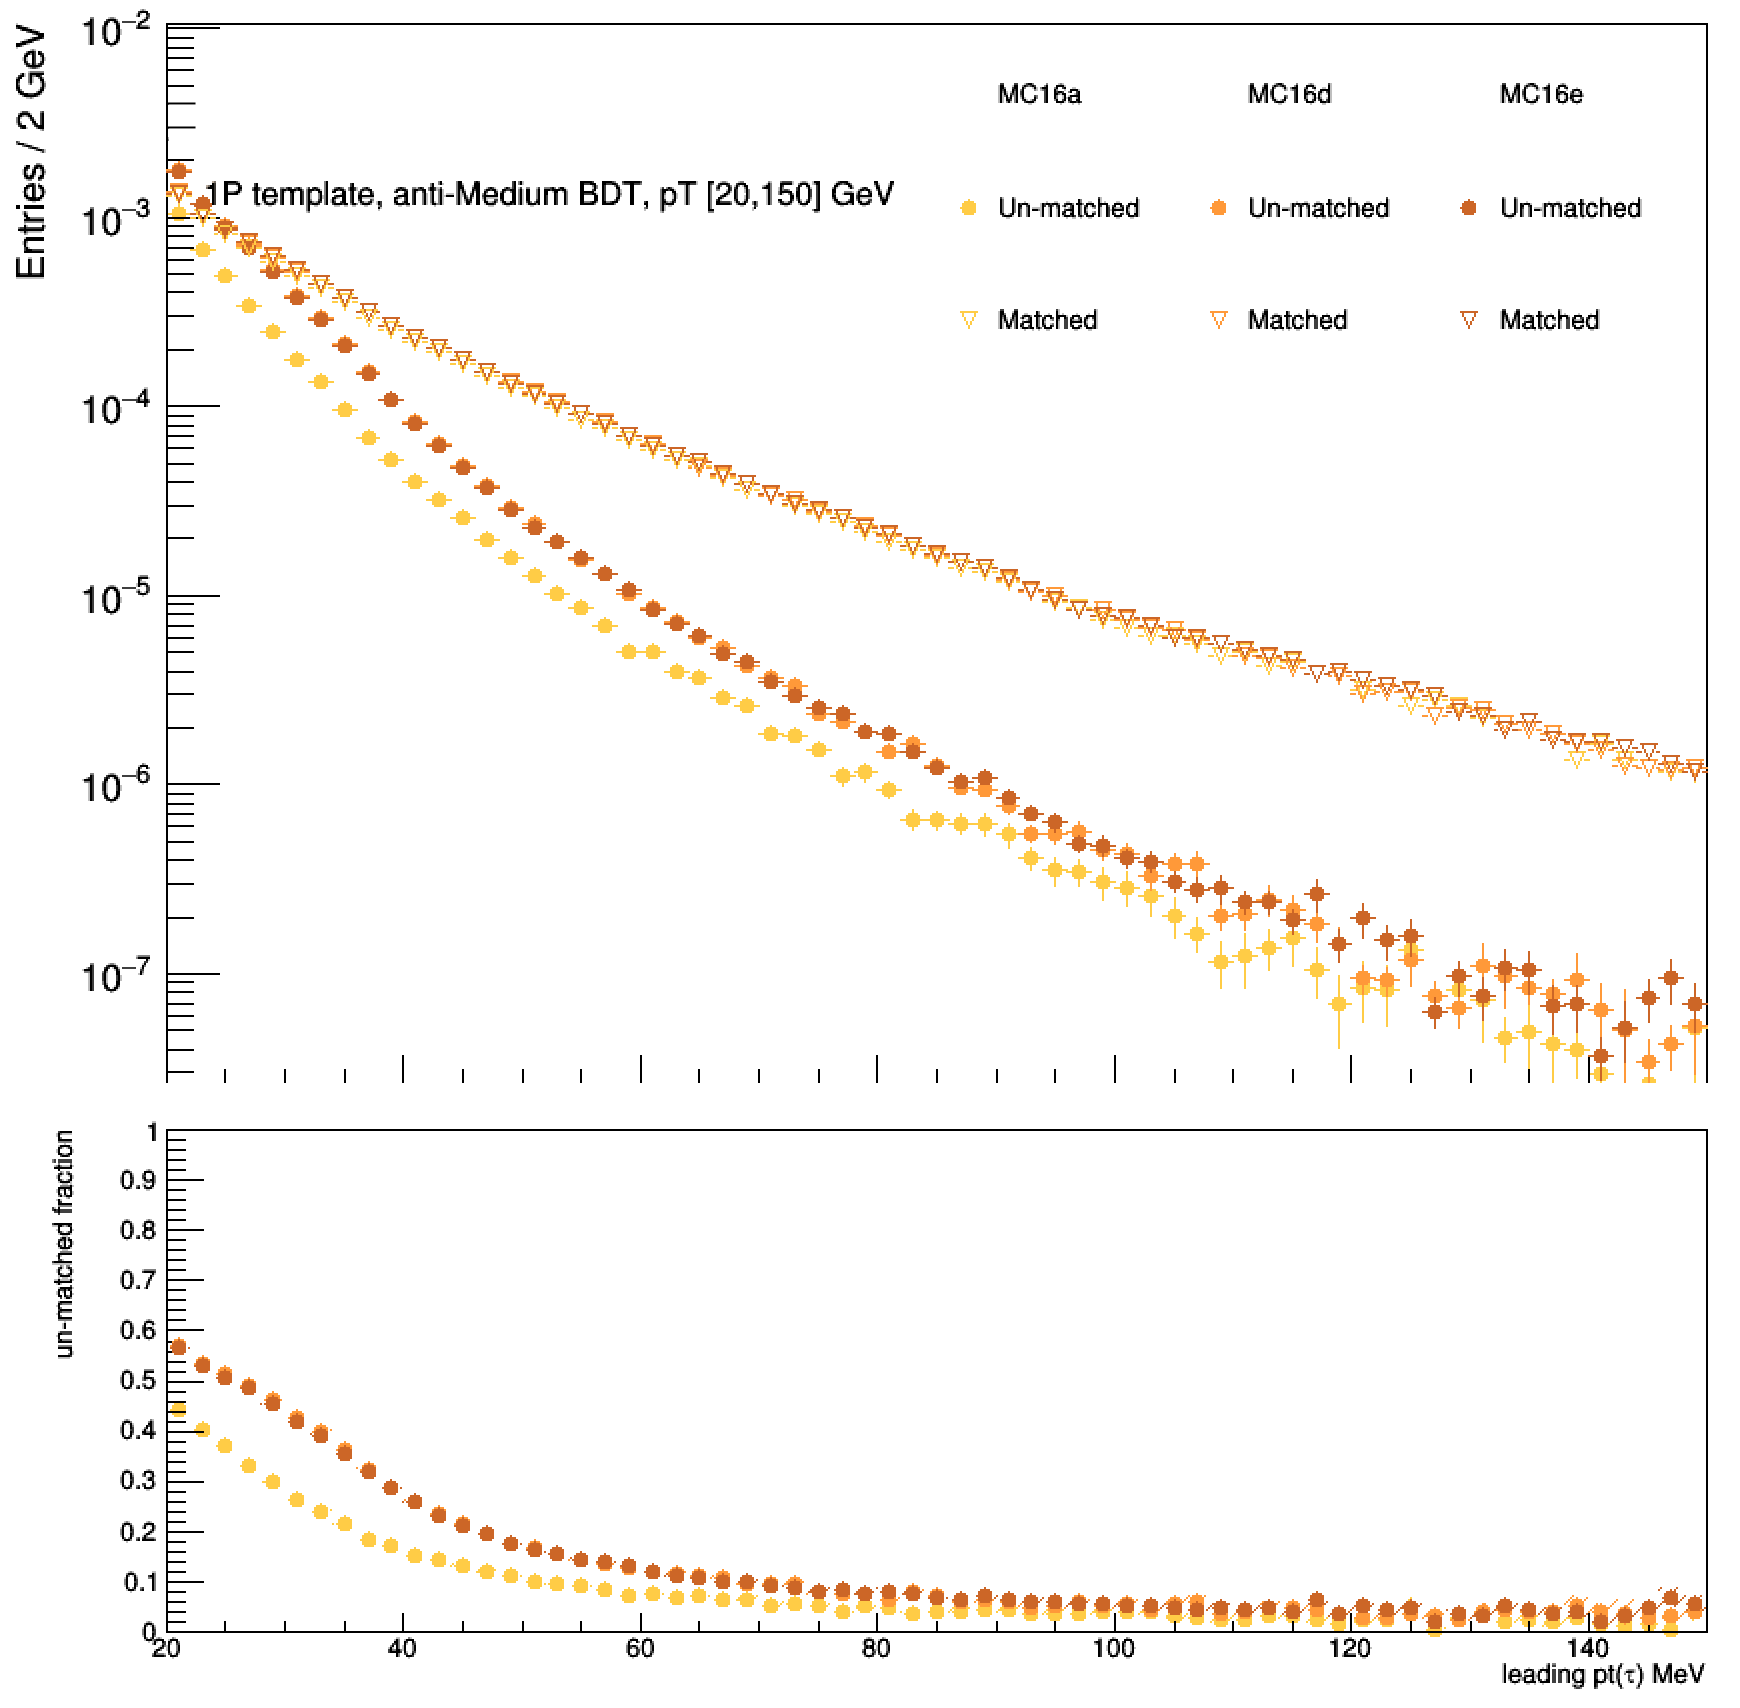
\includegraphics[width=0.45\textwidth]{FakeTau/AOD/AOD_pt_comp_Zjets}}\hspace{0.03\textwidth}
			\subbottom[]{
				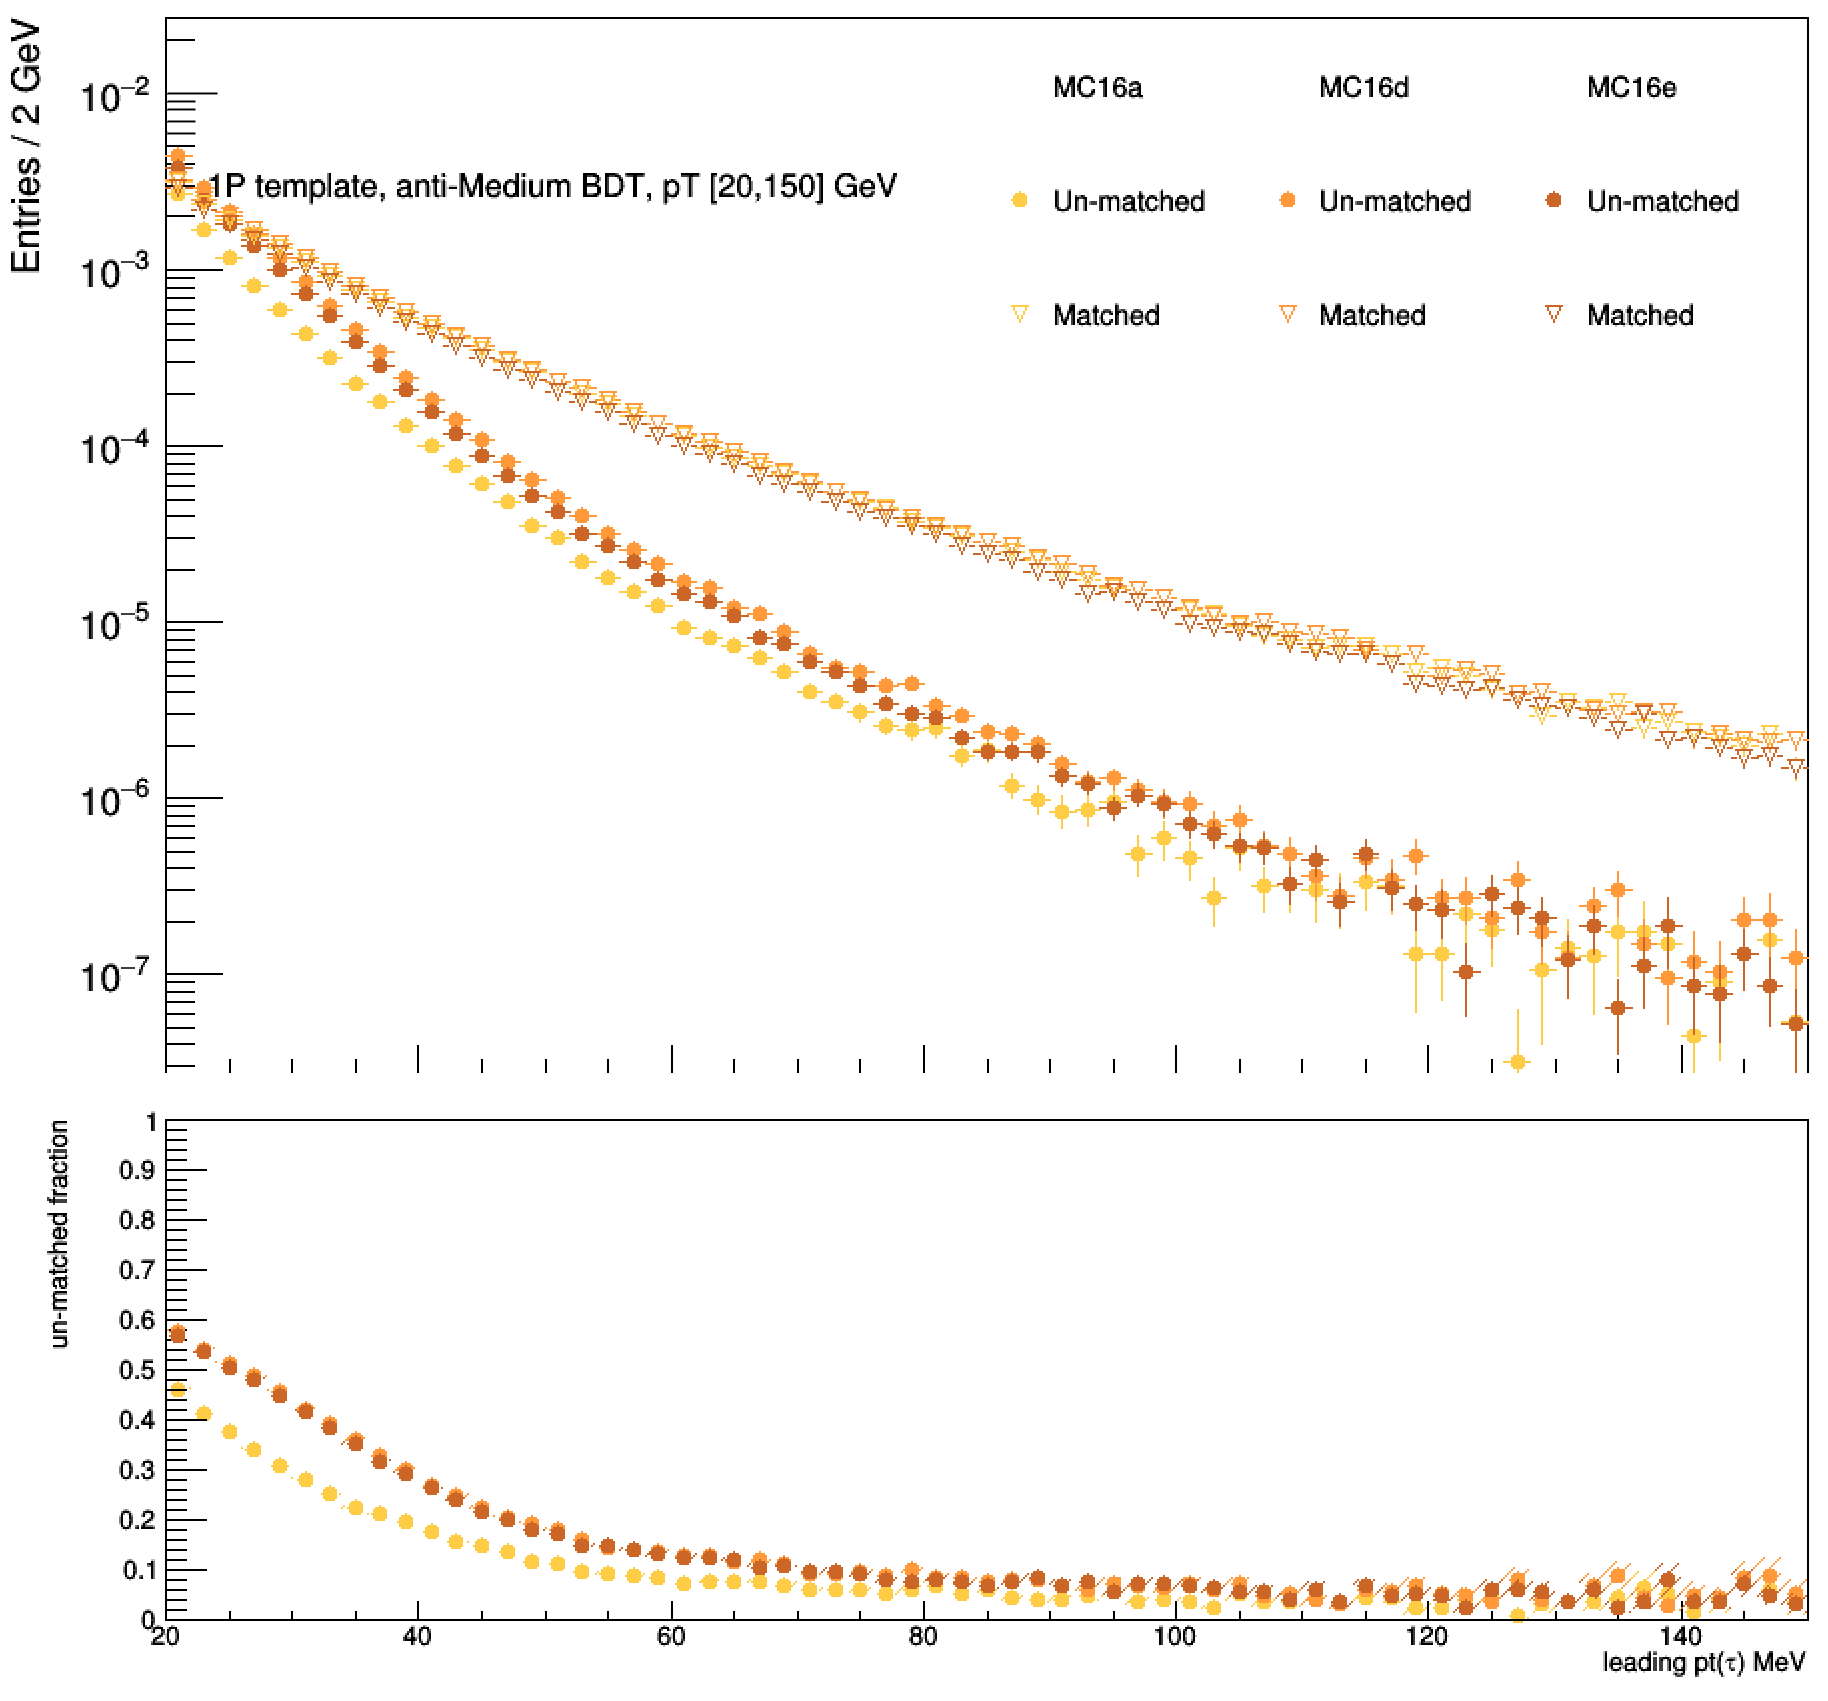
\includegraphics[width=0.45\textwidth]{FakeTau/AOD/AOD_pt_comp_Wjets}}\hspace{0.03\textwidth}
			\subbottom[]{
				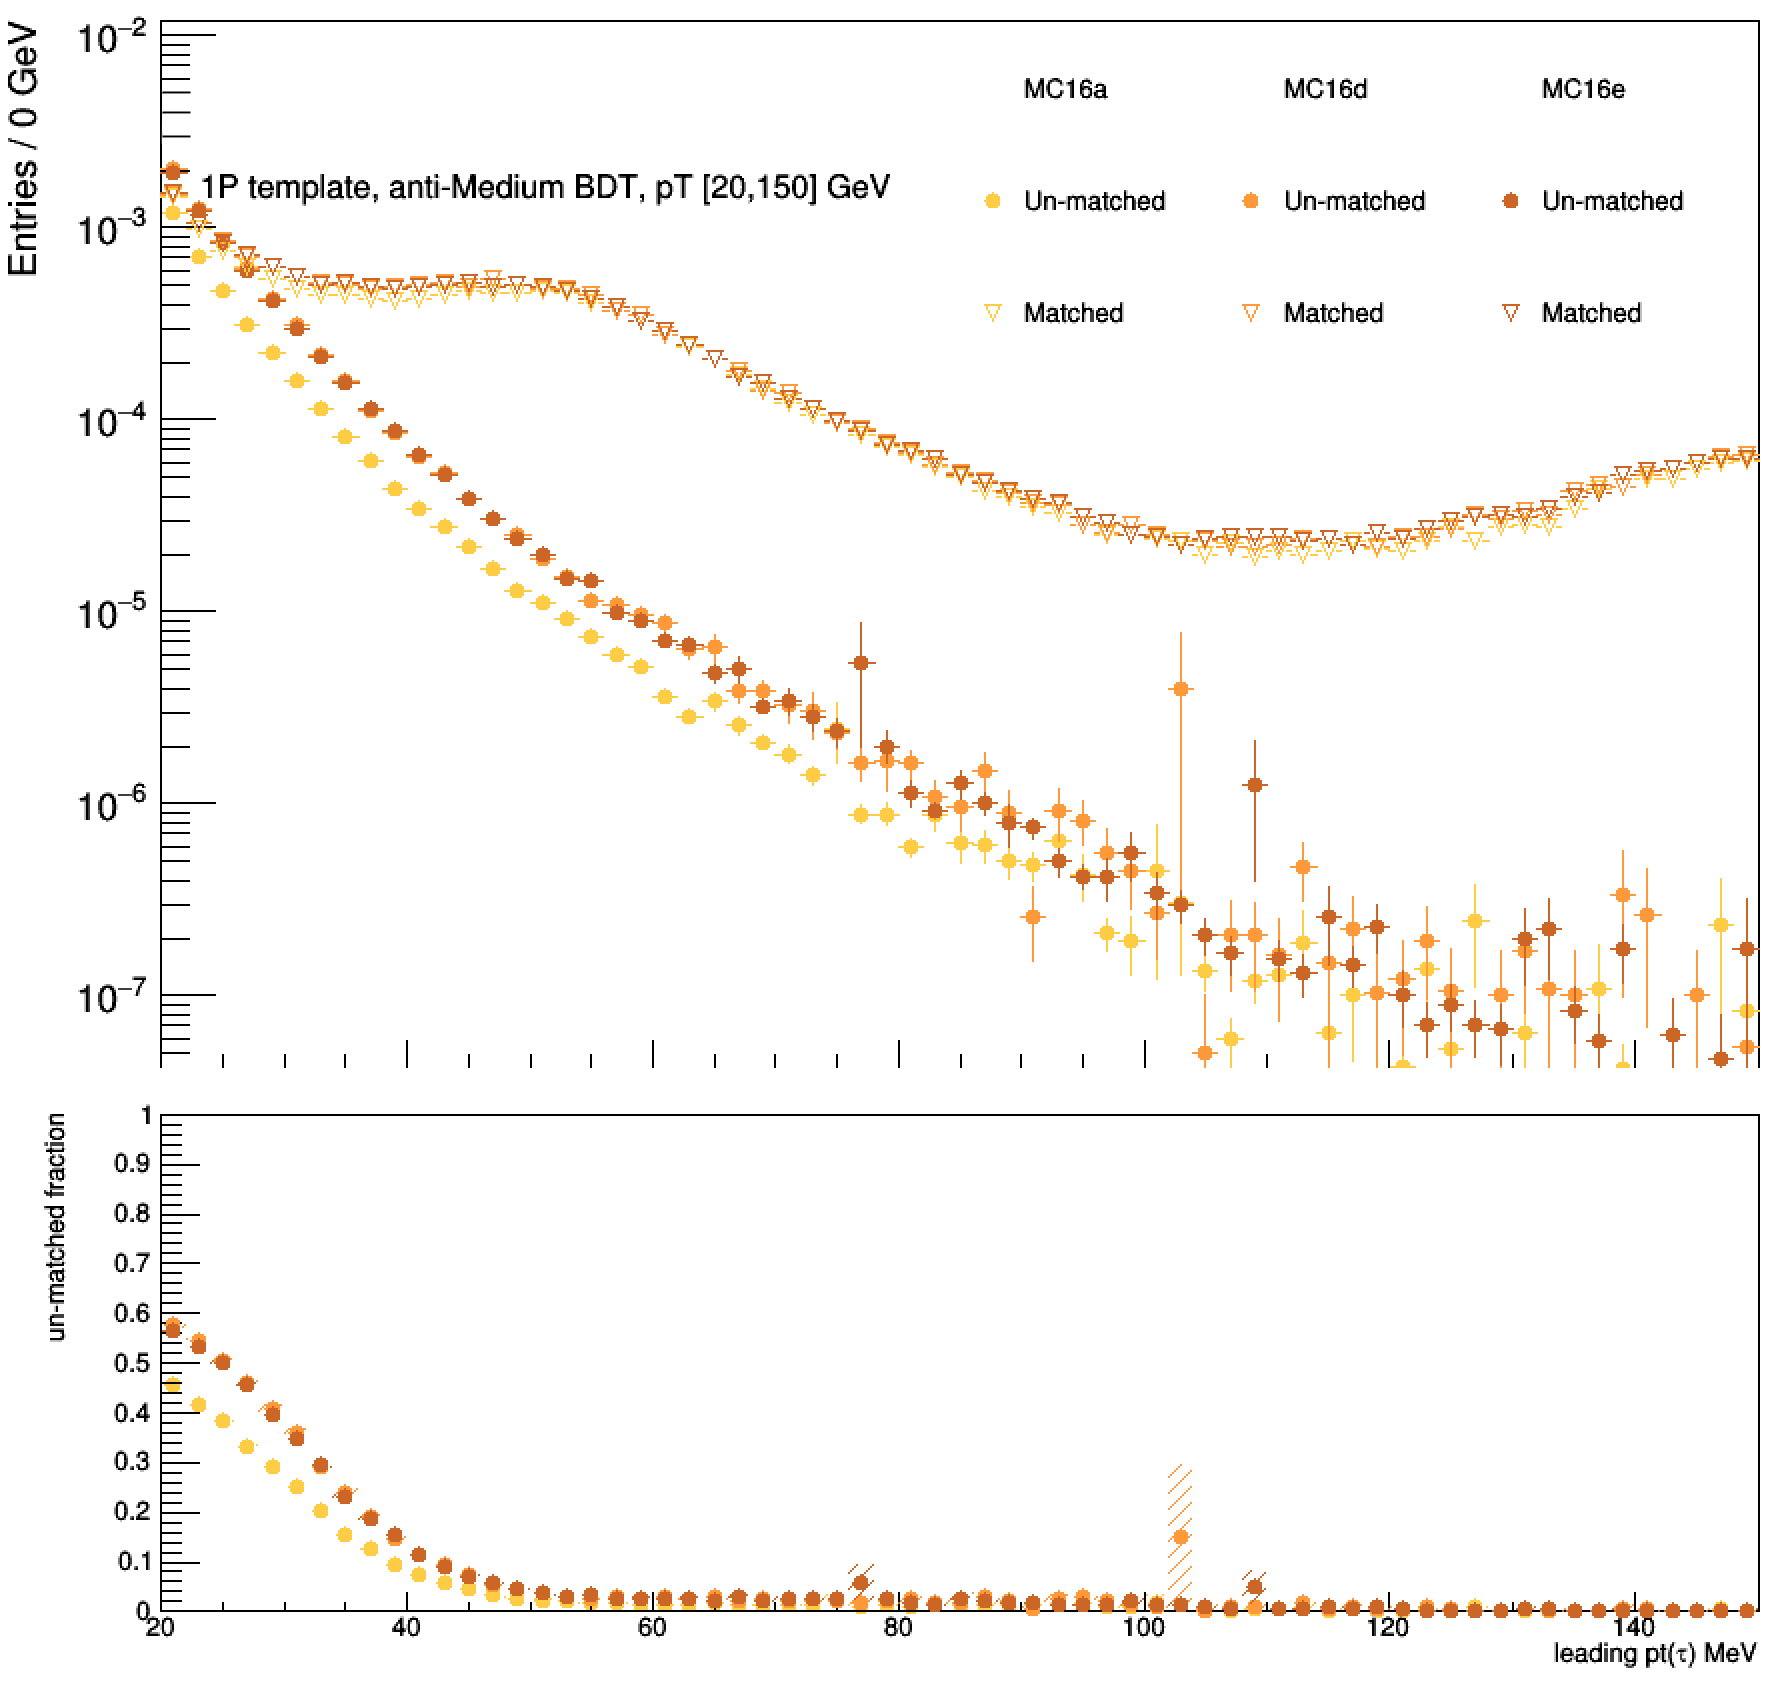
\includegraphics[width=0.45\textwidth]{FakeTau/AOD/AOD_pt_comp_dijet}}\hspace{0.03\textwidth}
		\end{center}
		\caption{Figures showing the \pt\ distribution for leading \htau\ candidates for matched (quark+gluon) and un-matched candidates in the (a) Z+jets, (b) W+jets and (c) di-jet samples for MC16a, MC16d and MC16e campaigns. The bottom plots shows the ratio of matched to un-matched candidates for each campaign for the respective samples.}
	\label{fig:mc16aVSmc16dVSmc16e}
	\end{figure}		
	Un-matched objects are defined as the candidates that fail the truth-matching procedure. Figure~\ref{fig:mc16aVSmc16dVSmc16e} shows the distribution of highest visible fake-taus \pt\ per event for matched (i.e. quark and gluon) objects against the same distribution for the un-matched objects for all \ac{MC} campaigns. 
	The ratio plot below the \pt\ distributions shows that the un-matched objects have a higher multiplicity in the low \htau\ \pt\ region and decrease with increasing transverse momentum. 
	Furthermore, the fraction of of un-matched candidates seems to increase with increasing mean number of interaction per bunch-crossing (\mubar). The different \ac{MC} samples shown in Figure~\ref{fig:mc16aVSmc16dVSmc16e} are generated with the different pileup conditions, where MC16a, MC16d and MC16e correspond to \mubar$=24.5$, \mubar$=41.9$ and \mubar$=40.9$ with luminosities of 36.2 \fb , 44.3 \fb\ and 58.4 \fb , respectively. 
	The relative higher number of un-matched candidates present in the samples with higher \mubar\ implies a direct correlation between un-matched candidates and \mubar. A considerably significant number of un-matched candidates can, thus, be attributed to \ftau\ pile-up jets.
	
	\subsection*{p$_T$ dependence}
	
	\label{subsec:pt_reweight}
	\begin{figure}[!hbt]
		\begin{center}
			\subbottom[]{
				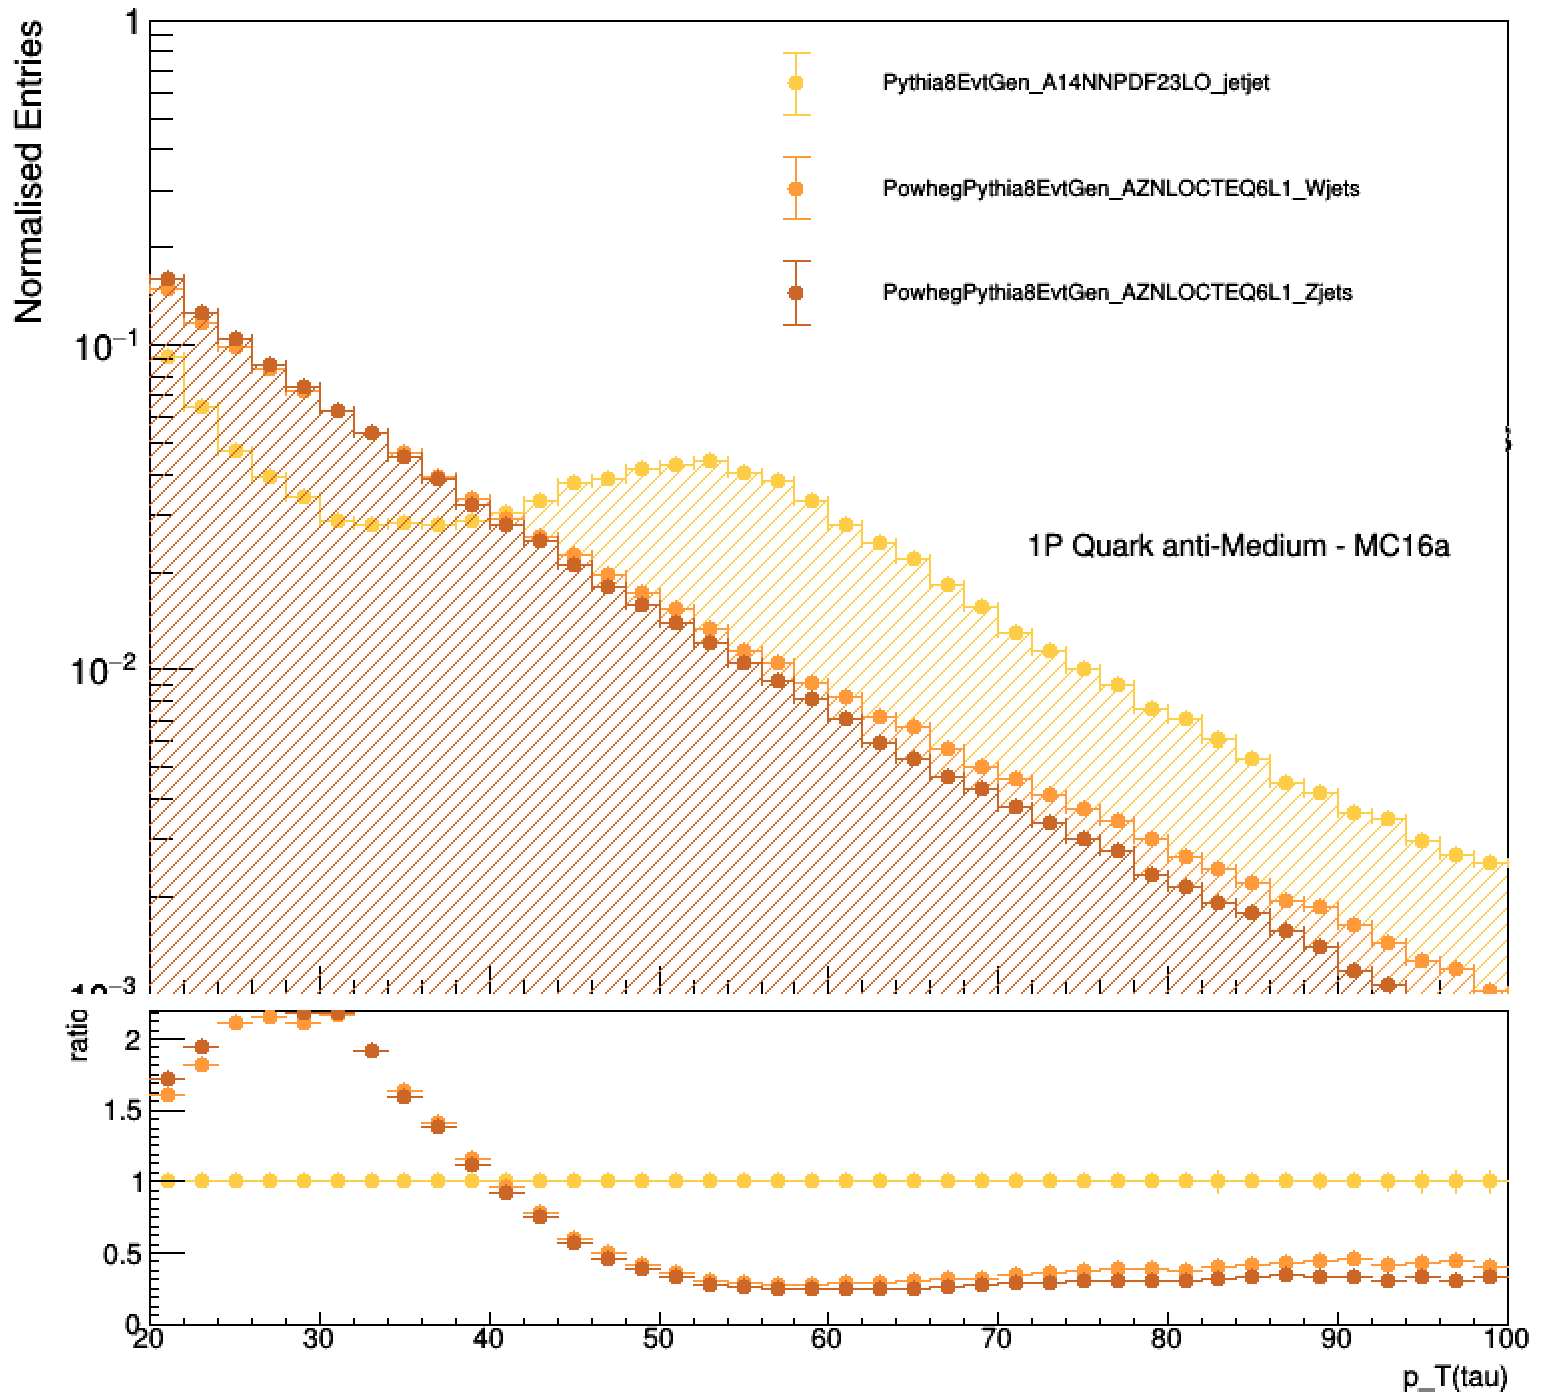
\includegraphics[width=0.45\textwidth]{FakeTau/AOD/MC16a/AOD_q_pt}}\hspace{0.03\textwidth}
			\subbottom[]{
				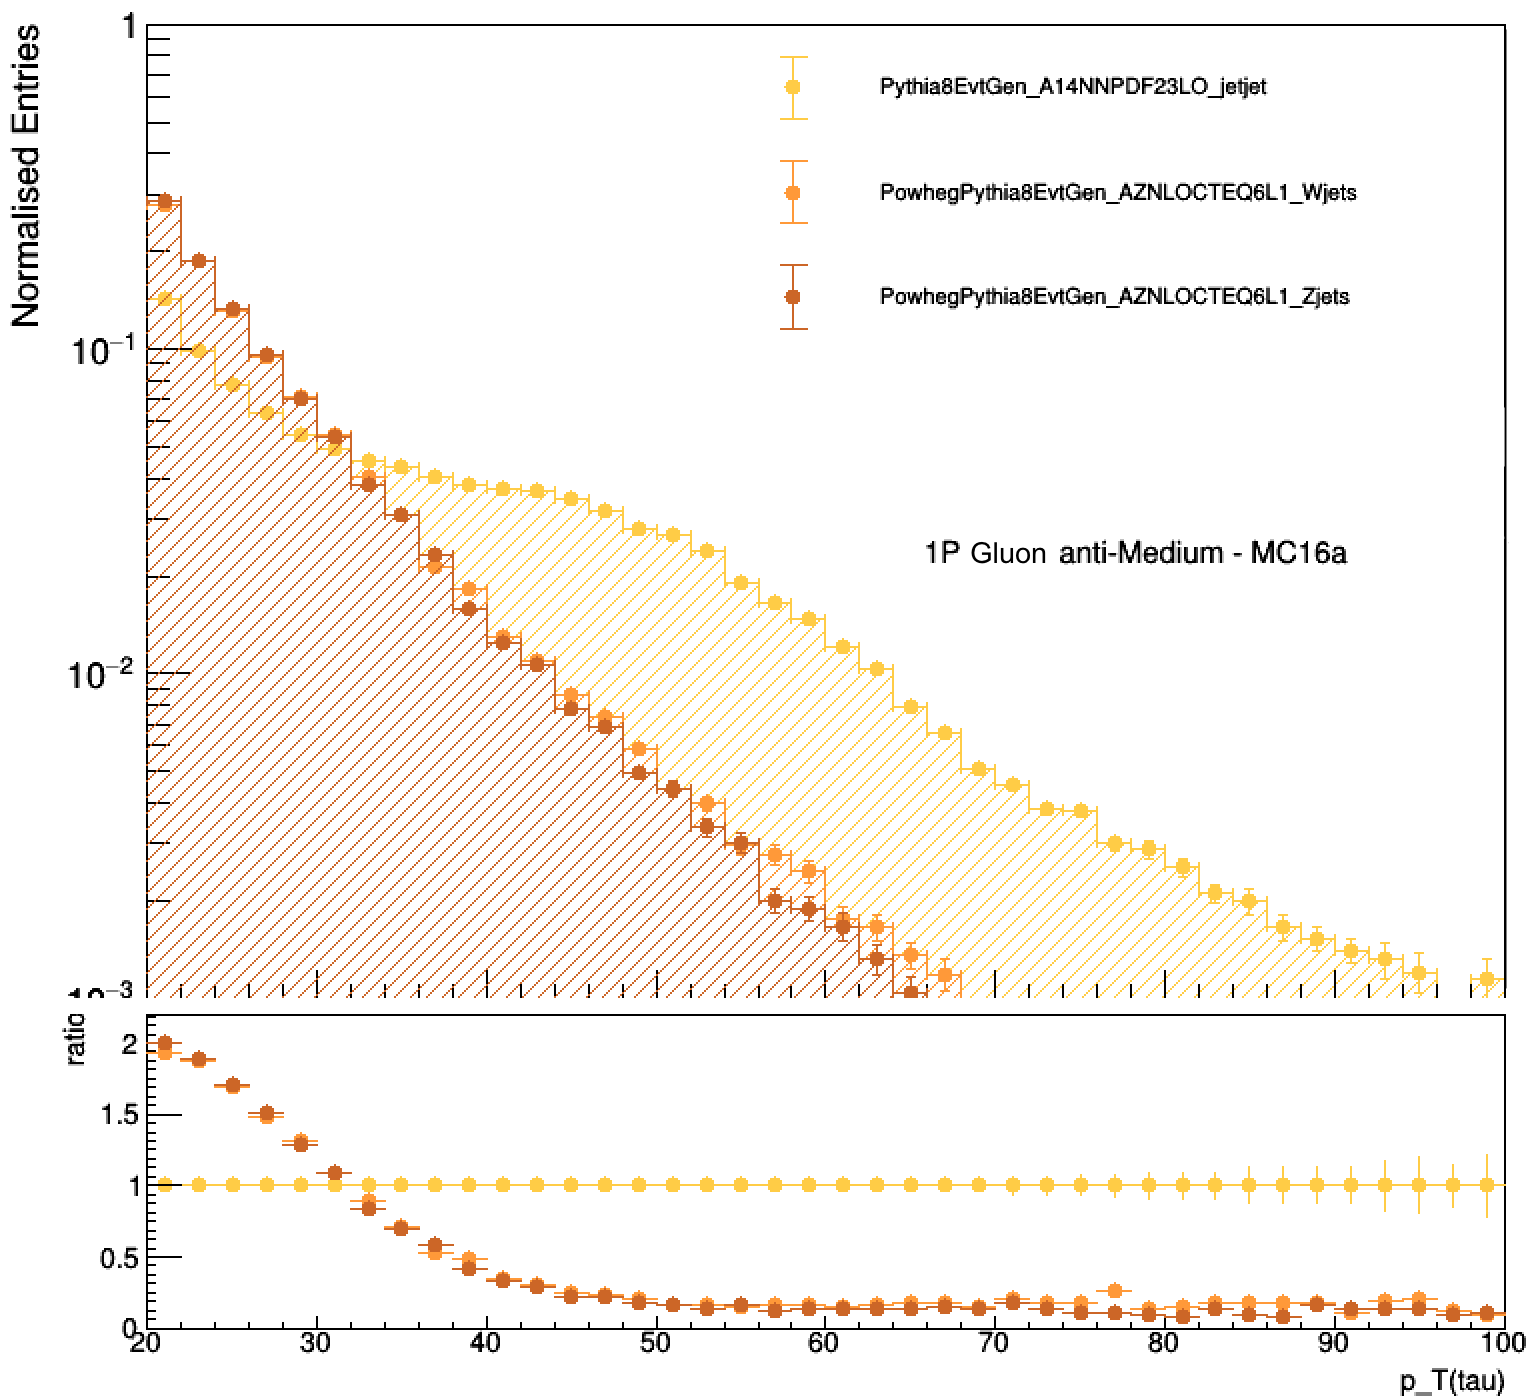
\includegraphics[width=0.45\textwidth]{FakeTau/AOD/MC16a/AOD_g_pt}}\hspace{0.03\textwidth}
			%\subbottom[]{
			%	\includegraphics[width=0.3\textwidth]{example-image-c}}\hspace{0.03\textwidth}
		\end{center}
		\caption{\htau \pt\ distribution plots for truth matched fake-tau candidates,\ie\ to quarks (left) and gluons (right) in dijet, Z+jet and W+jet samples. Histograms have been normalised to unity to show differences in shape. Bottom plot shows the ratio between the dijet and the other sample's \pt\ distribution.}
	\label{fig:MCtemp_qgu}
	\end{figure}		
	Figure~\ref{fig:MCtemp_qgu} shows the MC quark and gluon (left and right plots respecitvely)
	 %and un-matched (b) 
	 \pt\ distributions extracted from Z+jets, W+jets and di-jet samples for the jet-initiated fake-tau object. As seen, different samples have different kinematic distributions for these tau-faking objects, which in turn affects their corresponding jet width distributions. 
	A boosted visible \htau\ object can have a narrower jet width compared to a lower \pt\ object since the tracks from the boosted object will tend to be closer. Furthermore, when comparing the data samples to \ac{MC} samples for \ac{FF} interpolation the Z$\rightarrow\mu\mu$ region will more closely match the \Zjets\ sample's kinematic properties then the \Wjets\ or di-jets \ac{MC} samples, for instance. However, all samples described in the previous section (both \ac{HP} and \ac{LP}) are needed to construct the resulting templates. 
	The dependence (or bias) caused by the different \pt\ distributions between the samples on the jet widths must therefore be isolated and removed. 
	There are two main effects that need to be addressed. 
	
	The first effect to consider is the direct dependence of \pt\ on the jet width of the \htau\ object. 
	To that end, the \pt\ of the fake-\htau\ candidates is separated into bins, as shown by Table~\ref{tab:pt_bins}.
	The jet width templates and FF values need to thus, be derived for each \pt\ bin. This ensures that regions of different kinematic properties are treated and evaluated separately.
	
	\begin{table}[!hbt]
	\caption{visible \htau\ \pt\ binning used for derivation of templates and \ac{FF} values.}
	\begin{center}
	%\documentclass[10pt]{article}
%\usepackage[usenames]{color} %used for font color
%\usepackage{amssymb} %maths
%\usepackage{amsmath} %maths
%\usepackage[utf8]{inputenc} %useful to type directly diacritic characters
%\begin{document}
%\begin{table}[]
\begin{tabular}{cc}
\hline 
Min & Max \\ \hline \hline
20 & 30 \\
30 & 40 \\
40 & 60 \\
60 & 90 \\
90 & 150 \\
150 & inf \\ \hline 
\end{tabular}
%\end{table}
%
%\end{document}
	\end{center}
	\label{tab:pt_bins}
	\end{table}
	Each \pt\ bin must be "fine-binned" in intervals of 1 \gev, whereas the jet width distributions should range between 0-0.3 and have bin widths of 0.01. For instance, the 20-30 \gev\ \pt\ bin would have:
	\begin{itemize}
	\item \pt\ fine-binning:
		$$\{20,21,22,23,24,25,26,27,28,29,30\}$$
	\item jet width fine-binning:
		$$\{0.00,0.01,0.02,0.03,0.04,0.05,0.06,0.07,0.08,0.09,0.10,0.11,0.12,0.13,0.14,0.15,0.16,$$
		$$0.17,0.18,0.19,0.20,0.21,0.22,0.23,0.24,0.25,0.26,0.27,0.28,0.29,0.30\}$$
\end{itemize}	 
	Further dependences on other quantities taken into consideration and are isolated into further bins ( or requirements), as shown by Table~\ref{tab:FTTF_requierements}. 
	\begin{table}[!hbt]
	\caption{Further available requirements for further isolation of jet width dependence. Any combination of these requirements can be done and studied, where each combination would result in corresponding set of FF values and jet width templates. Note "*" corresponds to the options that have so far been studied.}
	\begin{center}
	%\documentclass[10pt]{article}
%\usepackage[usenames]{color} %used for font color
%\usepackage{amssymb} %maths
%\usepackage{amsmath} %maths
%\usepackage[utf8]{inputenc} %useful to type directly diacritic characters
%\usepackage{multirow}
%
%\begin{document}
%\begin{table}[]
\resizebox{\textwidth}{!}{\begin{tabular}{cccccccc}
\hline 
Prong & BDT min & BDT WP  & RNN min & RNN WP & WP region & JVT cut & Trigger Pass \\ \hline \hline
\multirow{2}{*}{1*}  & 0.00 & Loose & 0.00 & Loose & \multirow{2}{*}{pass} & \multirow{2}{*}{no JVT cut*} & \multirow{2}{*}{no requirement*} \\
  & 0.05* & Medium*  & 0.01* & Medium* &  &  &  \\
3*  & 0.50 & Tight  & 0.05* & Tight & fail* & some JVT cut & passed\\ \hline 
\end{tabular}}
%\end{table}
%
%\end{document}
	\end{center}
	\label{tab:FTTF_requierements}
	\end{table}
	"Prong" signifies the number of charge tracks associated with the studied \htau\ vertex, and can either be 1 or 3 prong. "BDT WP" and "RNN WP" correspond to the the \ac{BDT} and \ac{RNN} identifier algorithm working points, respectively, and can be either \textit{Loose}, \textit{Medium} or \textit{Tight} as defined in Table~\ref{tab:BDT_RNN_eff}. The "BDT min" and "RNN min", corresponds to the minimum background rejection efficiency scores of the \ac{BDT} and \ac{BDT} identifier algorithms at which a \htau\ candidate is accepted. 
	% This is only relevant when the investigating the anti-region --- represented by the "WP region" column,  which can be either pass or fail for the SR-like region or anti-region respectively --- as the range of BDT (RNN) scores would go from the minimum BDT (RNN) score up to the BDT (RNN) WP considered.  
	The "JVT cut" selects for objects that have passed the \ac{JVT} algorithm~\cite{ATLAS-CONF-2014-018}, which is primarily used to suppress pileup jets. Finally the last possible selection displayed in the column "Trigger requirement" applies when a trigger requirement is requested to be passed by the \htau\ object.
	
	The second effect that needs to be considered is the different \pt\ distributions shapes between different samples.
	%The second method's goal is to remove the \pt\ effects between different samples. 
	The procedure used to minimise this effect is 
%	This is 
	generally referred to as \pt\ re-weighting and is performed as follows. 
	For MC samples comparison the samples are separated into two categories, one sample is used as "reference", while the rest are considered "variable" samples.
%	\begin{wrapfigure}{R}{.5\textwidth}
\begin{figure}[!hbt]
	\begin{center}
			\subbottom[]{
				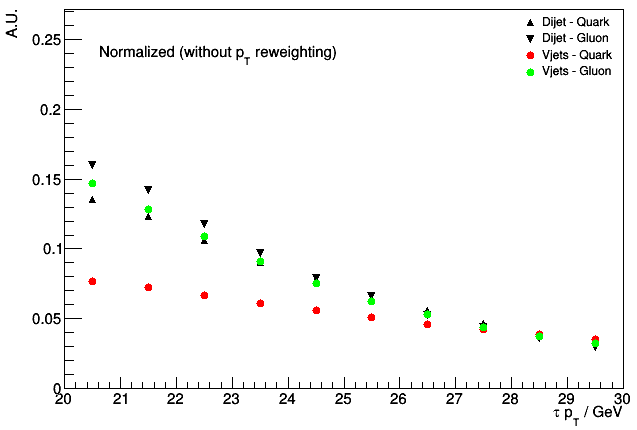
\includegraphics[width=0.45\textwidth]{FakeTau/AOD/Reweighting_comparison_without_reweighting.png}}\hspace{0.05\textwidth}
			\medskip			 
			 %\smallskip\par
			 \subbottom[]{
				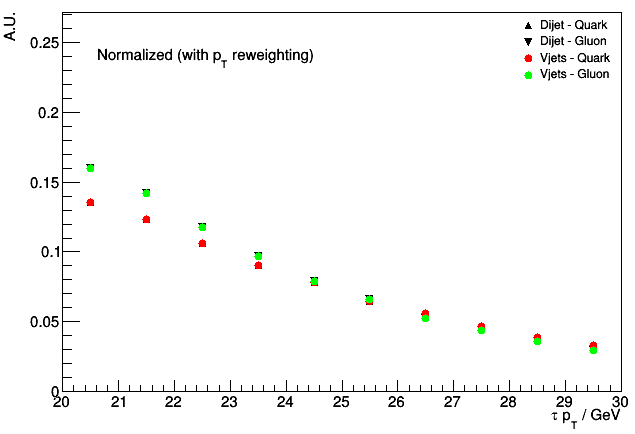
\includegraphics[width=0.45\textwidth]{FakeTau/AOD/Reweighting_comparison_with_reweighting.png}}\hspace{0.05\textwidth}
		\end{center}
		\caption{Top plot shows the distribution of \htau\ \pt\ for the truth match \htau\ to quark (black) and gluon (red) for dijet and V+jets (W+jets and Z+jets merged). Bottom plot shows the same distributions after implementing the re-weighting procedure with respect to the dijet sample.}
	\label{fig:pt_reweighting_comp}
	\end{figure}	
%\end{wrapfigure}	
	The "reference" sample \pt\ distribution is used as distribution to which the other ("variable") samples are re-weighted to.
	Because the different parton \pt\ distributions (quark, gluon, un-matched...) need to be independently re-weighted, the procedure must be performed for each parton.
	Each sample's parton full \pt\ distribution can thus be derived and plotted in histograms of 1 GeV \pt\ bins. 
	The distributions are normalised to unity before the re-weighting is performed, as to be independent of any scaling factors applied to the distribution.
	By comparing the "reference sample" distribution to the "variable sample", an weight for each \pt\ bin can be derived for each sample. 
	This event weight can then be used to re-weight the "variable sample" \pt\ distribution to the "reference sample" one.
	In contrast, when comparing the MC samples (di-jet, W+jet and Z+jet ) to the FF interpolation data regions (multijet and Z$\rightarrow\mu\mu$), the quark, gluon and un-matched candidates are independently re-weighted to the \pt\ distribution of the FF interpolation regions as well as to the region of interest.
	%When comparing MC samples the \pt\ distributions of the relevant partons to be studied is derived in each samples and are normalised to unity. A "scaling factor" can thus be derived as an event weight to re-weight the parton distribution of the "variable sample" 
	%Therefore, when considering quark, gluon and un-matched candidates, their templates are re-weighted 	
	An example of \pt\ re-weighting is shown for the quark template \pt\ in Figure~\ref{fig:pt_reweighting_comp}. Plot (a) shows the quark and gluon \pt\ distributions between the different samples in the \pt\ bin $\in[20,30]$ before re-weighting. As described above, the distributions have been normalised to unity to clearly show the differences in the \pt\ distribution between samples. In Plot (b) the same distributions, with the \pt\ re-weighting procedure applied are shown. The \pt\ re-weighting changes the distribution shape to make them coincide with the appropriate parton. 
	% shows the the same distributions but with the \pt\ re-weighting procedure applied, thus showing that the shape of the distributions coincide. 
	
	Figure~\ref{fig:qgu_jetwidth_reweighting} shows the effect of \pt\ re-weighting on the jet width distributions for quarks (a), gluons (b) and un-matched (c) MC templates. For all templates the \pt\ re-weighting results in only a very small shift of the jet width distribution. This indicates that the \pt\ distribution shape between processes only has a small effect for these samples.
	\begin{figure}[!hbt]
	\begin{center}
			\subbottom[]{
				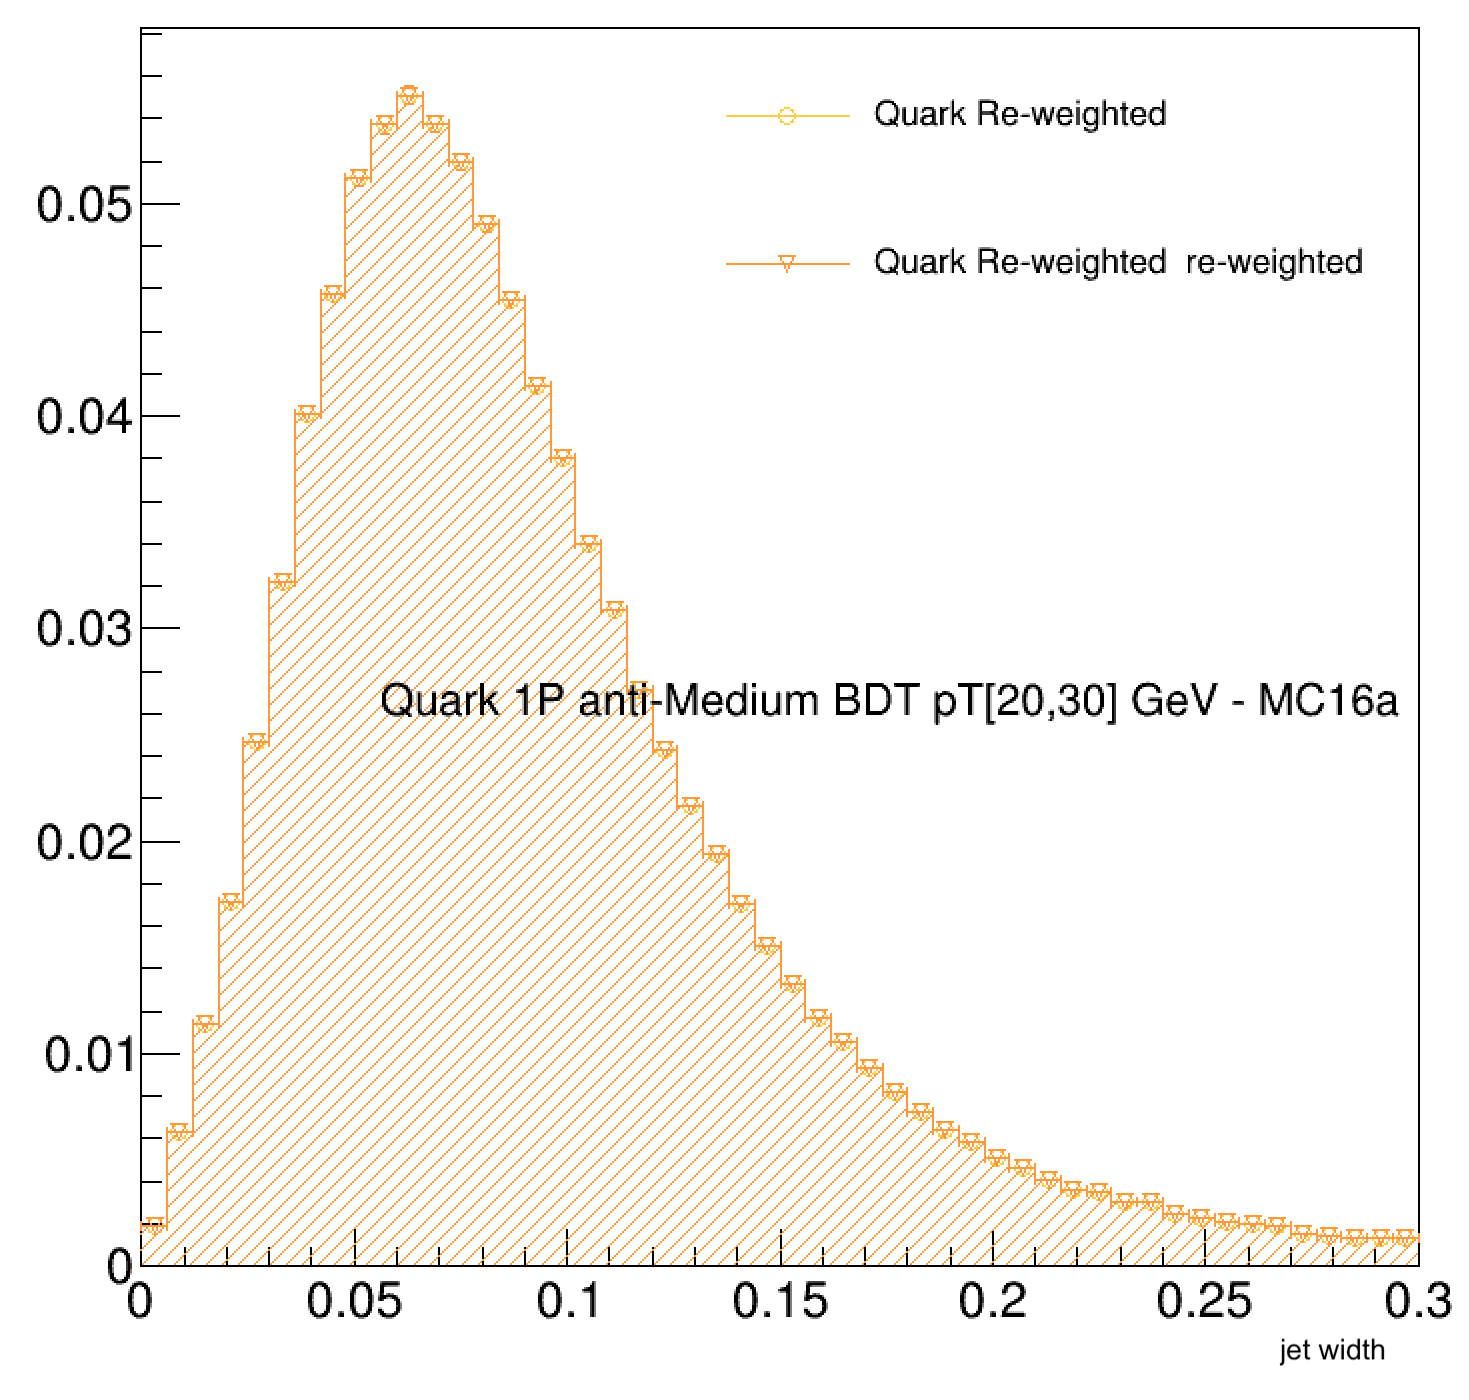
\includegraphics[width=0.45\textwidth]{FakeTau/AOD/MC16a/AOD_q_ptrew}}\hspace{0.03\textwidth}
			\subbottom[]{
				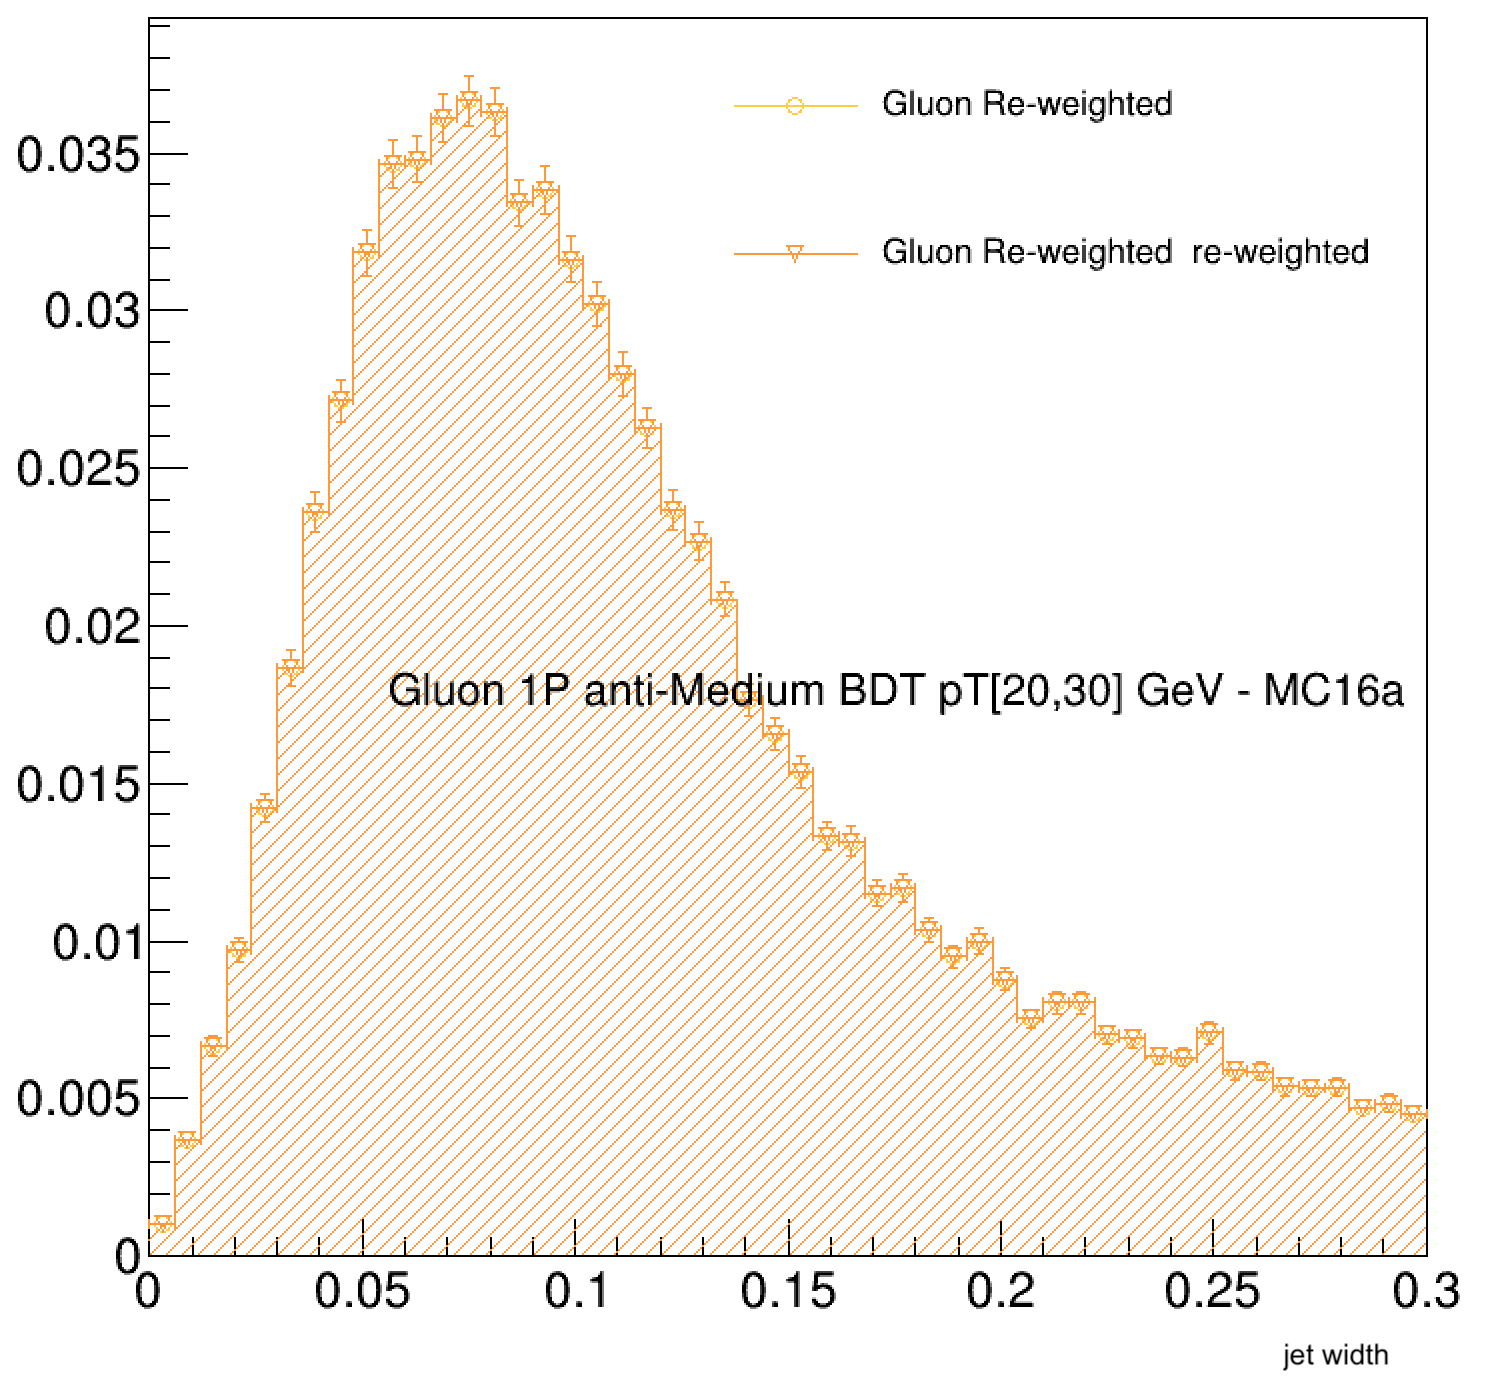
\includegraphics[width=0.45\textwidth]{FakeTau/AOD/MC16a/AOD_g_ptrew}}\hspace{0.03\textwidth}
			\subbottom[]{
				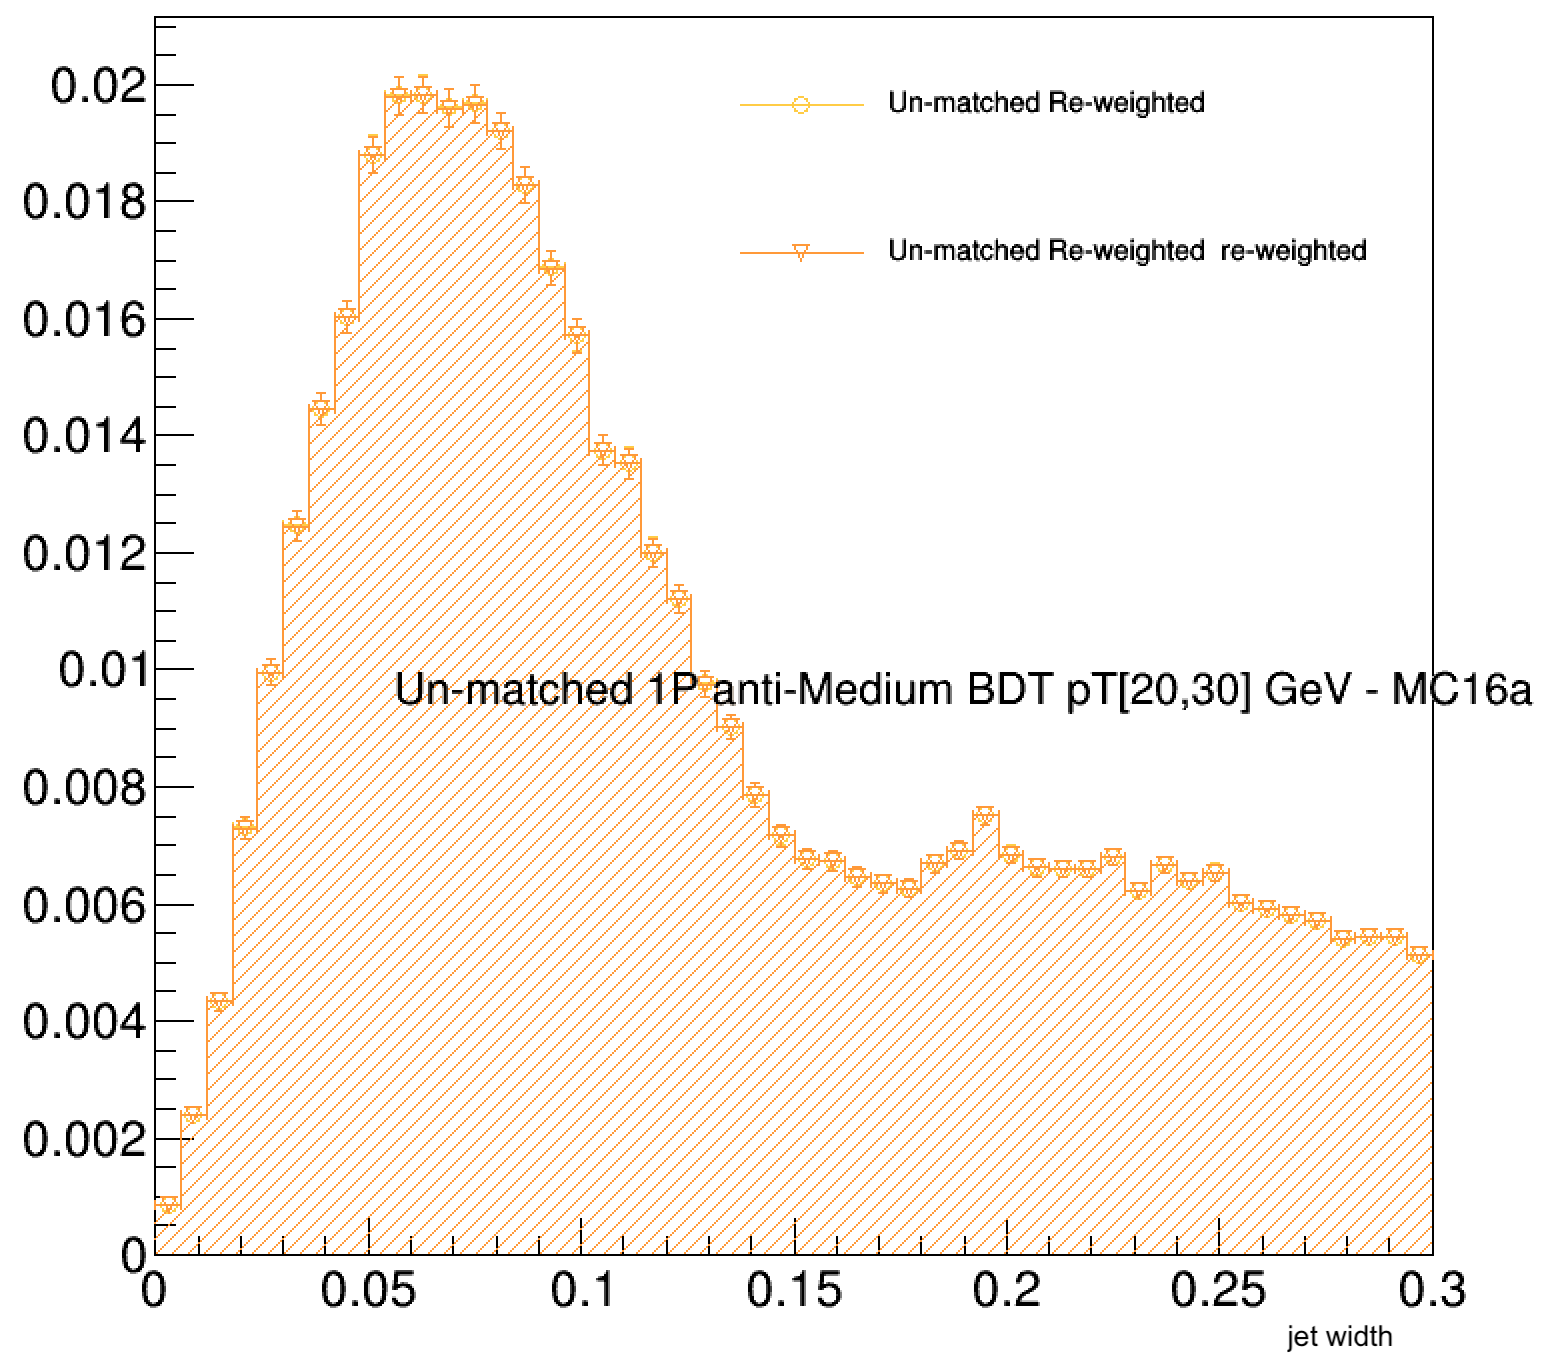
\includegraphics[width=0.45\textwidth]{FakeTau/AOD/MC16a/AOD_u_ptrew}}\hspace{0.03\textwidth}
		\end{center}
		\caption{The effect of \pt\ re-weighting on MC16a Z+jet sample using dijet sample as "reference" on the track-based jet width templates of quark, gluon and un-matched candidates are shown in plots (a), (b) and (c), respectively. All plots correspond to one prong 20-30 GeV \htau\ candidates which fail the "Medium" \ac{BDT} working point. }
	\label{fig:qgu_jetwidth_reweighting}
	\end{figure}		
	
	\subsection{Derived Analysis Object Data samples}
	\label{sec:DxAOD}
	%In this section the issues found when using AOD samples to describe the properties of analysis level objects are discussed and templates for the derivation samples that resulted from the studies of the issues with the AOD are presented.
	%In the above sections it was shown that the Universality of the Fake Factor method is observable when using very relaxed selections and un-calibrated objects.	
	
	The concepts described above for the derivation and application of \ac{FF} are intended to be developed for use in many different types of analyses. 
	To that end it is important to ensure that general analyses selections and object calibrations, or any other tools applied at analysis level, do not unexpectedly affect the quark fraction or jet width templates, and if so they must be studied and understood for the proper application of the universal \ac{FF} method.
	
	\begin{figure}[!hbt]
		\begin{center}
			\subbottom[]{
				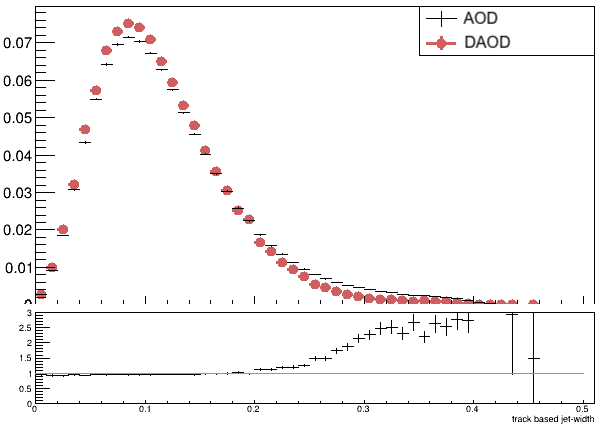
\includegraphics[width=0.45\textwidth]{FakeTau/AOD/AODvsDAOD/MariovsPetar-mc_Quark_nominal_17_1p_notmedium_zmcut_notautrig_20to30_AND_EtaIncl_tau_0_seed_TrackWidthPt1000.png}}\hspace{0.03\textwidth}
			\subbottom[]{
				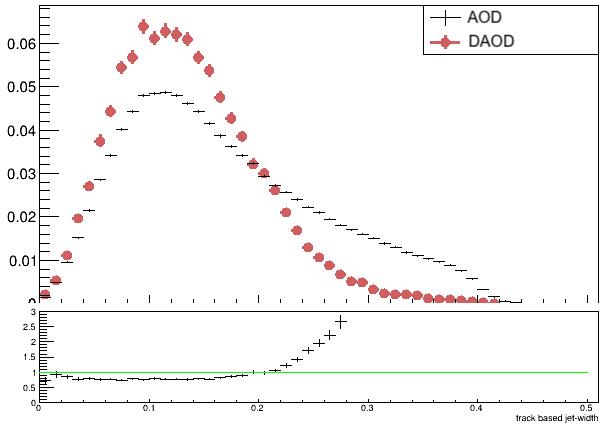
\includegraphics[width=0.45\textwidth]{FakeTau/AOD/AODvsDAOD/MariovsPetar-mc_Gluon_nominal_17_1p_notmedium_zmcut_notautrig_20to30_AND_EtaIncl_tau_0_seed_TrackWidthPt1000.png}}\hspace{0.03\textwidth}
				\subbottom[]{
				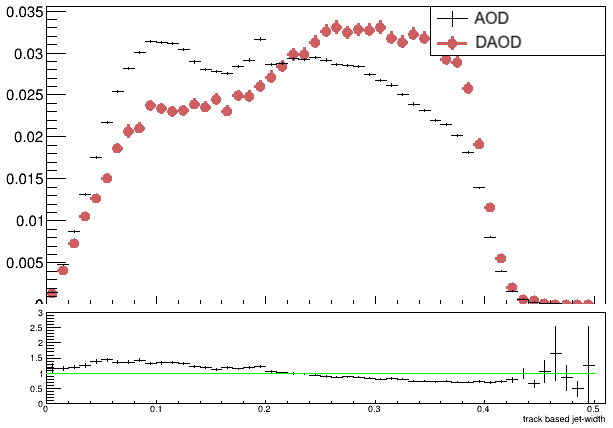
\includegraphics[width=0.45\textwidth]{FakeTau/AOD/AODvsDAOD/MariovsPetar-mc_Unmatched_nominal_17_1p_notmedium_zmcut_notautrig_20to30_AND_EtaIncl_tau_0_seed_TrackWidthPt1000.png}}\hspace{0.03\textwidth}
		\end{center}
		\caption{Comparison between AOD and DAOD samples for quark (a), gluon (b) and un-matched (b) track-based jet width templates. The bottom plot shows the ratio between the AOD and DAOD distribution.}
	\label{fig:xOAD_vs_DxAOD}
	\end{figure}	
	Figure~\ref{fig:xOAD_vs_DxAOD} shows the track based jet width distributions between two differently processed \ac{MC} samples in the anti-\textit{Medium} working point \ac{BDT} region (\ie\ accepting events which fail the \textit{Medium} \ac{BDT} \htau\ requirement), for 1-prong \htau\ in the \pt\ bin $\in[20,30]$.
	 One of the samples shown is an \ac{AOD} (blue), while the second is a \ac{DAOD} sample (red).
	\ac{DAOD} (also called "derivation") is the name given to \ac{AOD} samples that have also been processed through "derivation selections". 
	Significant discrepancies in the track based jet width distributions are observed, indicating that the \ac{DAOD} sample introduces some bias to the tau kinematics that needs to be fully understood.	
	
	The samples used for \ac{ATLAS} physics analyses are \ac{DAOD}. This is because \ac{DAOD} samples include selection and calibrations that are essential for the accurate reconstruction and kinematic properties of particle objects.
	%The basic selections and calibrations applied to \ac{AOD} samples to generate the \ac{DAOD} are essential analysis use in \ac{ATLAS}. 
	The most relevant and common processing procedures applied to \ac{DAOD} samples are the \htau\ object calibration, the overlap removal procedure, and implementation of tighter selection cuts.
	 All of these procedures are discussed in more detail below. 
	  %\ac{DAOD} samples are \ac{AOD} samples that have undergone further processing, such as object calibration, overlap removal and tighter selection cuts (more detail on the \ac{DAOD} processing can be found in Section ~\ref{sec:DAOD_selection}).
	%Therefore a comparison between two sets of \ac{MC} derived track based jet width templates, where one set (which will be referred to as "nominal ntuples" in the text) is derived using the samples described in the previous section --- for which a very loose selection is used to avoid biasing the tau kinematics  in samples --- while the other set (which will be referred to as "analysis ntuples" in the text) is derived from the same set of samples, but has undergone some further calibrations and processes required by ATLAS for general analyses, can be done. 
	
	
%	Figure ~\ref{fig:xOAD_vs_DxAOD} shows this comparison for the quark, gluon and un-matched candidates derived from "nominal ntuples" (black) and "analysis ntuples" (red). For these plots the anti-Medium BDT region is observed, for 1-prong taus in the \pt\ bin $\in[20,30]$.
%	Some discrepancies in the templates shapes are observed, indicating that the "analysis ntuples", which are derived from the "nominal ntuples", do in fact posses some bias in the tau kinematics that is introduced by the tools used at analysis level.
	% The detail of the processes applied to the "analysis ntuples" will be described in details the next sections. 
	
		\subsection*{Object calibration}
	An important step of the visible \htau\ object reconstruction is the calibration. After the reconstruction of a \htau\ following the prescription described in Ref.~\cite{ATL-PHYS-PUB-2015-045}, the energy of the tau candidate is calibrated at the \ac{LC} scale, which corrects for calorimeter non-compensation and for the energy deposited in dead material or outside topological clusters of calorimeter cells.
	
	 \begin{figure}[!hbt]
		\begin{center}
			\subbottom[]{
				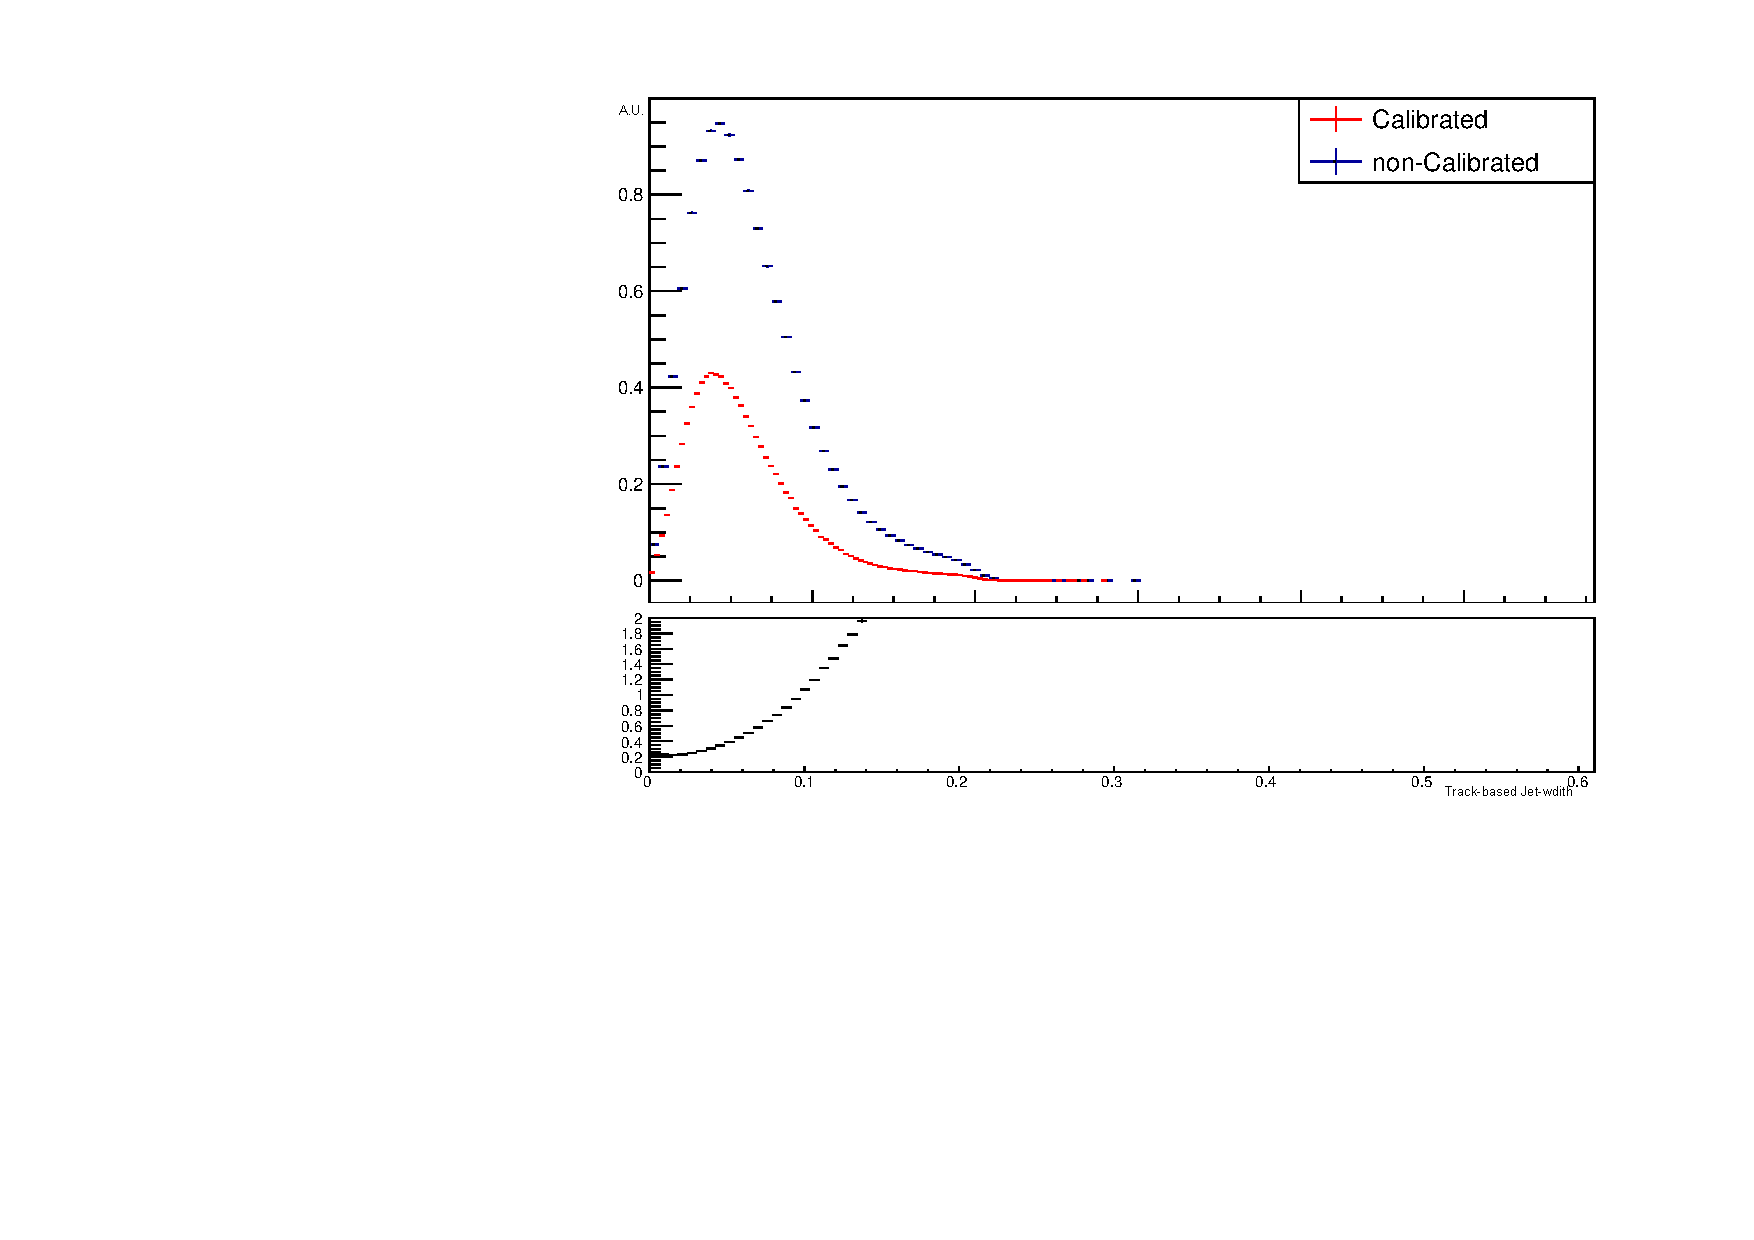
\includegraphics[width=0.45\textwidth]{FakeTau/AOD/TES/quark_1prong_[20,30]}}\hspace{0.03\textwidth}
			\subbottom[]{
				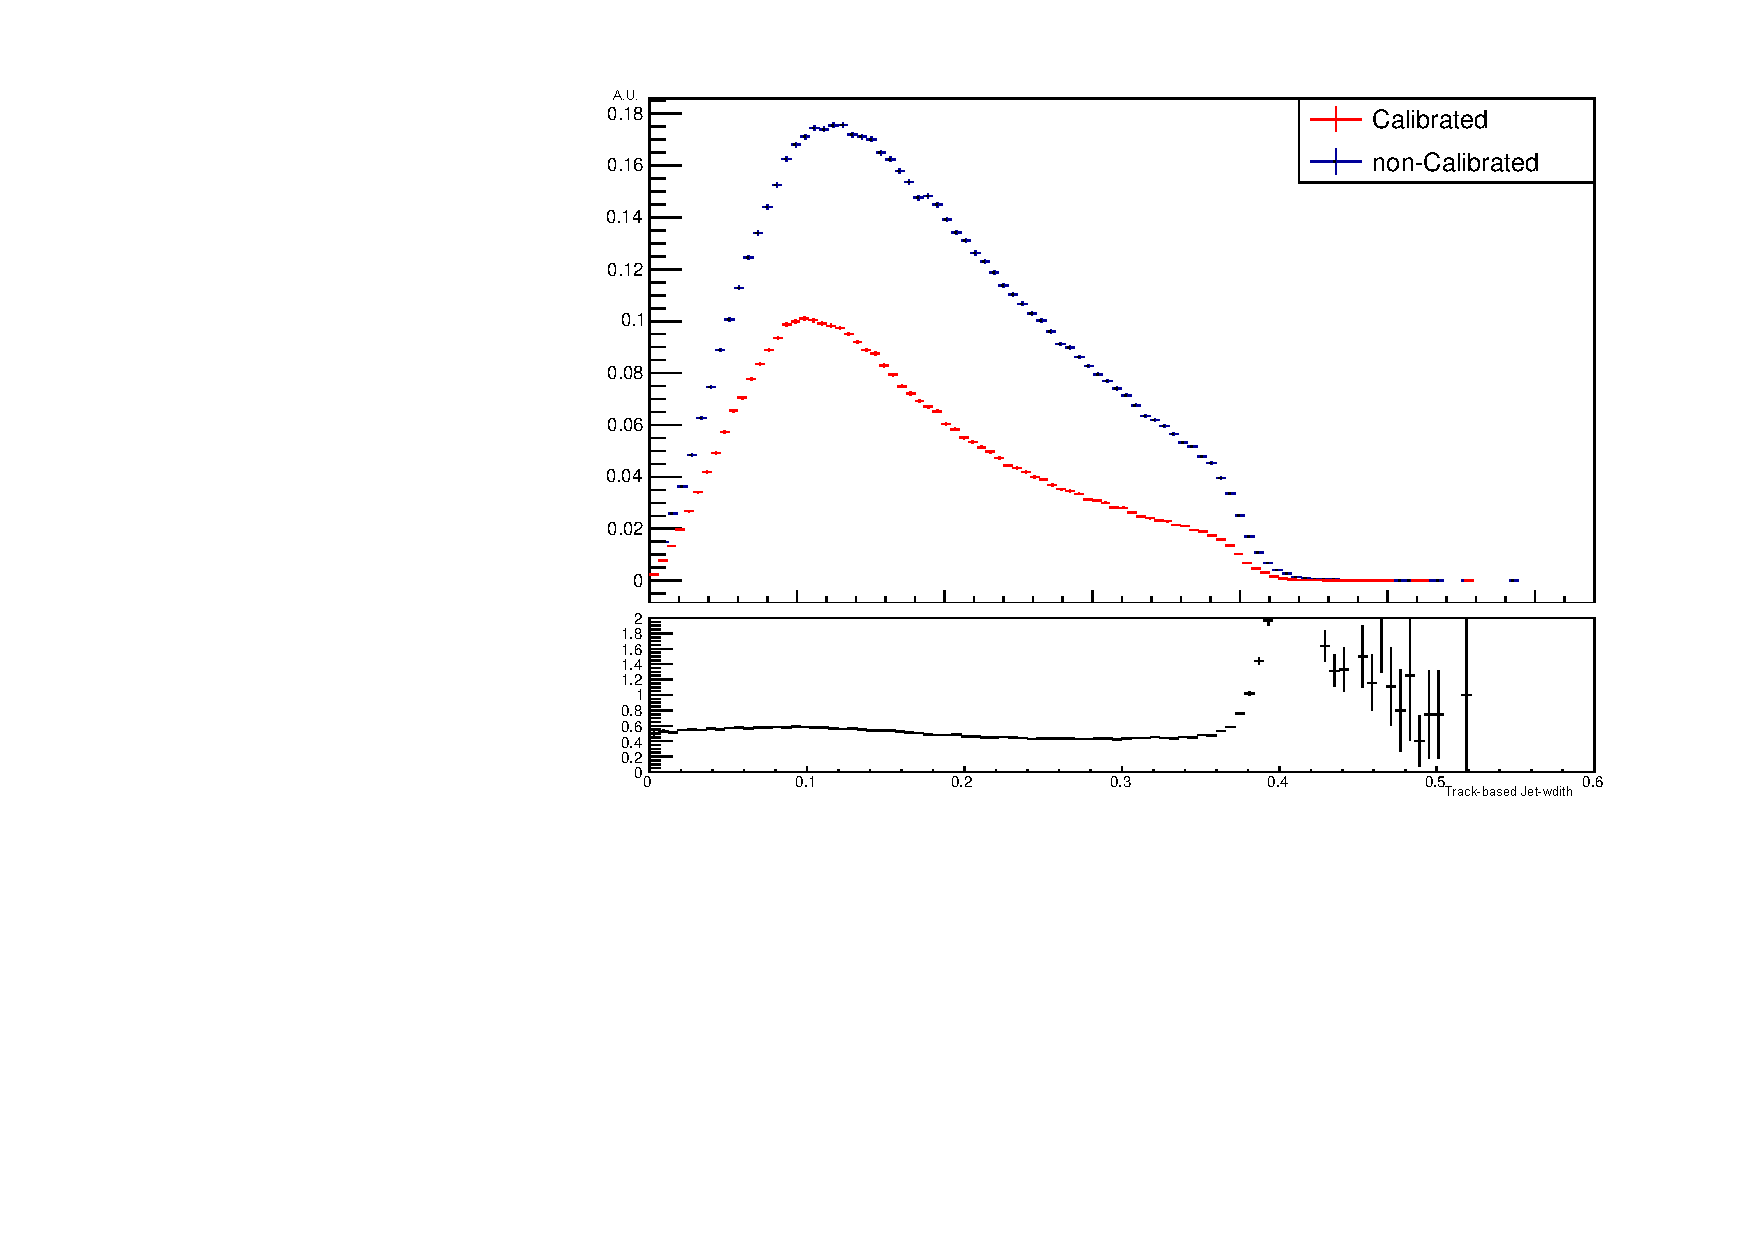
\includegraphics[width=0.45\textwidth]{FakeTau/AOD/TES/gluon_1prong_[20,30]}}\hspace{0.03\textwidth}
				\subbottom[]{
				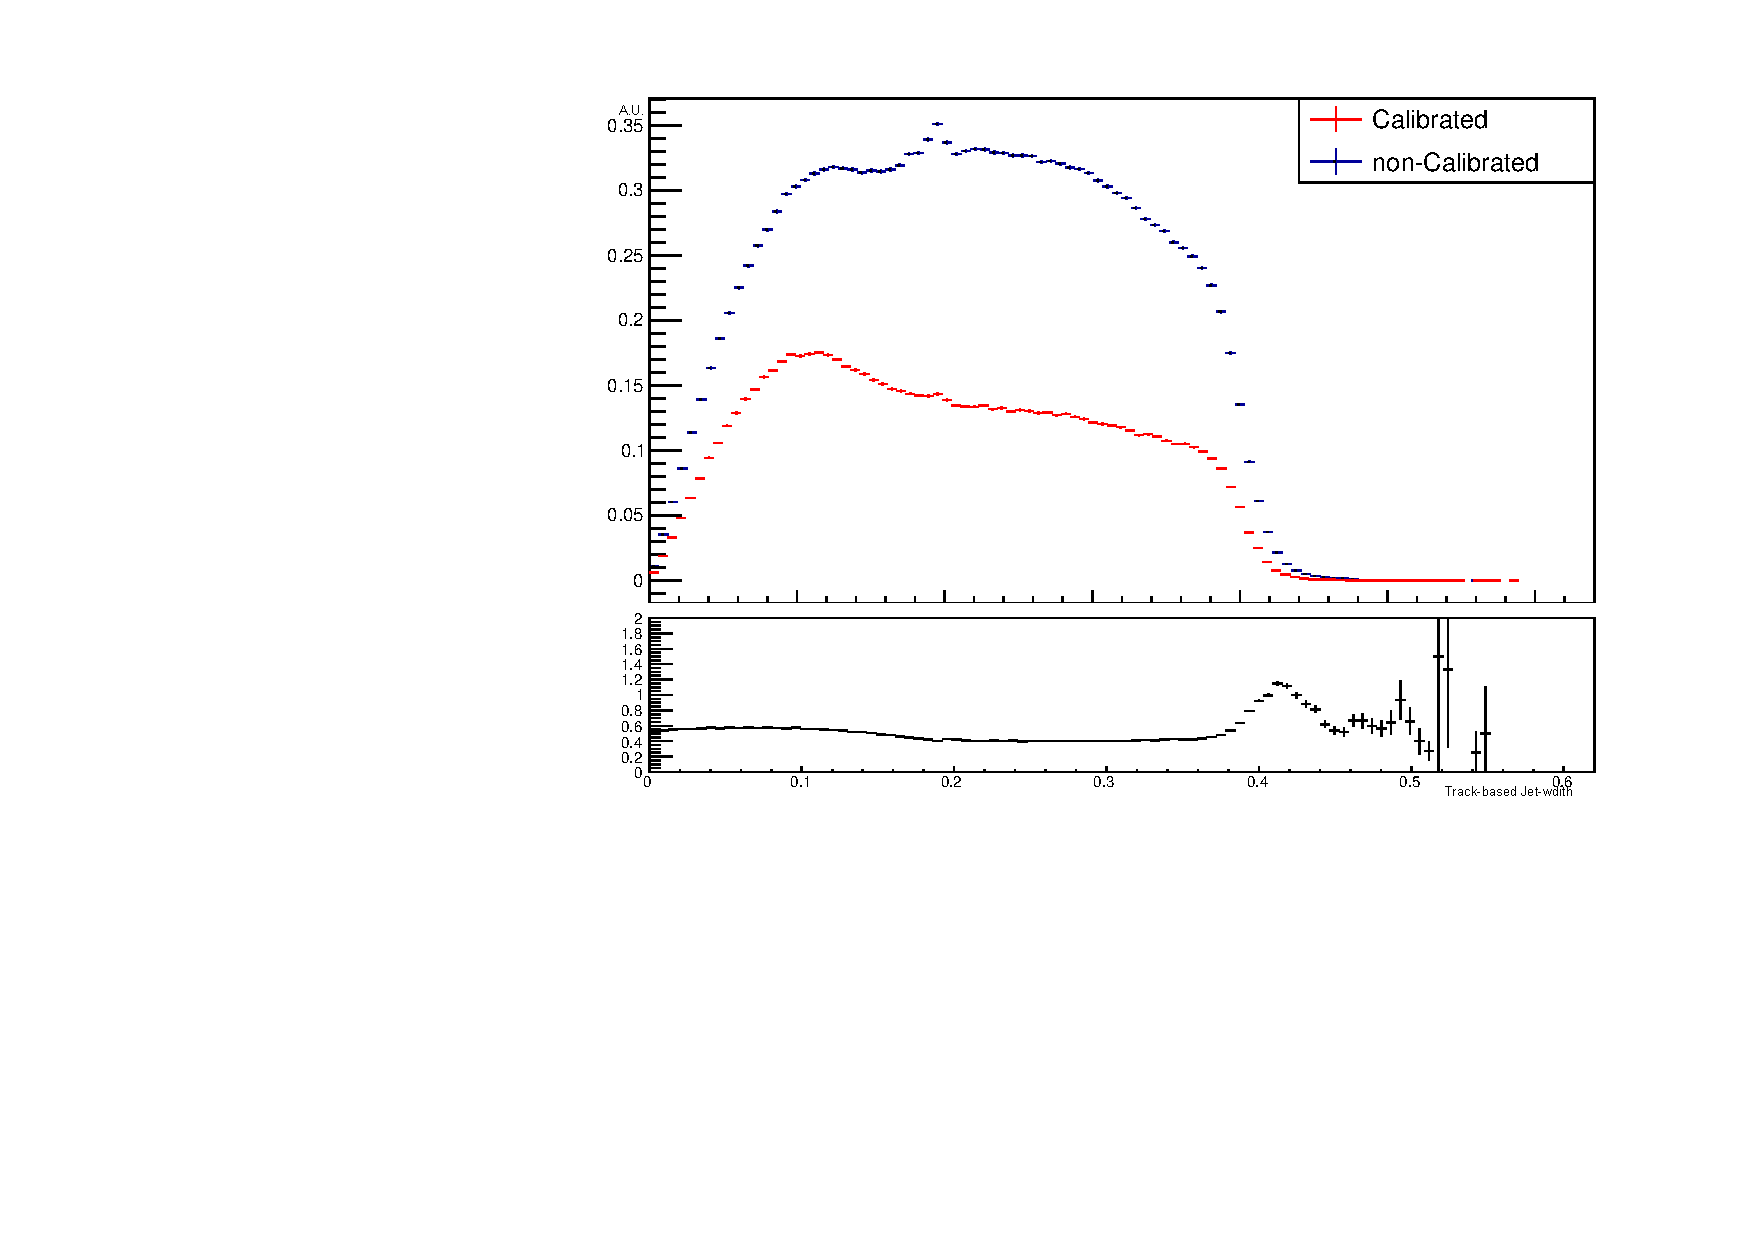
\includegraphics[width=0.45\textwidth]{FakeTau/AOD/TES/unmatched_1prong_[20,30]}}\hspace{0.03\textwidth}
		\end{center}
		\caption{Comparison of track-based jet width distribution of 1-prong \ftau\ (a) quarks, (b) gluons, and (c) un-matched candidates between an un-calibrated and calibrated $Z\rightarrow \mu\mu$ sample.}
	\label{fig:TES_comp}
	\end{figure}	
	The correction of the tau energy back to the true visible energy, via the application of the \ac{TES} can have significant affects on the kinematic properties of the reconstructed \htau. These effects must be taken into consideration when deriving templates of the \htau\ jet track-based jet width. The \ac{TES} calibration is generally performed when generating a "derivation" sample. Hence, the \htau\ objects contained in \ac{AOD} samples are not calibrated. 
	The effect of \ac{TES} calibration on the tau objects can be seen in Figure~\ref{fig:TES_comp} where the quark (a), gluon (b) and un-matched (c) track-based jet width templates are shown for calibrated and un-calibrated \htau\ objects. The figure shows the track based jet width templates for the different partons in the \pt\ bin $\in[20,30]$ in the Z$\rightarrow\mu\mu$ process. The large discrepancy observed in the quark template is due to the larger number of candidates with a track-based jet width value of 0, which when normalised to unity results in a relatively smaller distribution for the calibrated objects compared to the non-calibrated.
	
	
	\subsection*{Overlap removal procedure}
	\label{sec:ORprocedure}
	\begin{table}[!hbt]
	\caption{steps are performed in the listed order. only surviving objects participate in the subsequent steps.}
	\begin{center}
	%\documentclass[10pt]{article}
%\usepackage[usenames]{color} %used for font color
%\usepackage{amssymb} %maths
%\usepackage{amsmath} %maths
%\usepackage[utf8]{inputenc} %useful to type directly diacritic characters
%\begin{document}
%\begin{table}[]
\begin{tabular}{ccc}
\hline
\textbf{Reject Object} & \textbf{Against} & \textbf{Criteria} \\ \hline \hline
electron & electron & shared track, $p_{T_1}<p_{T_2}$ \\
tau & electron & $\Delta R<0.2$ \\
tau & muon & $\Delta R<0.2$ \\
muon & electron & is a calo-muon, shares ID track \\
electron & muon & shares ID track \\
photon & electron & $\Delta R<0.4$ \\
photon & muon & $\Delta R<0.4$ \\
jet & electron & $\Delta R<0.2$ \\
electron & jet & $\Delta R<0.4$ \\
jet & muon & N. Tracks $<$ 3, $\Delta R<0.2$ \\
muon & jet & $\Delta R<0.4$ \\
jet & tau & $\Delta R<0.2$ \\
photon & jet & $\Delta R<0.4$ \\
large-R jet & electron & $\Delta R<1.0$ \\
jet & large-R jet & $\Delta R<1.0$ \\ \hline
\end{tabular}
%\end{table}
%
%\end{document}
	\end{center}
	\label{tab:OR_req_table}
	\end{table}
	A common procedure employed, when running an analysis, to remove potentially overlapping objects, \ie\ a lepton that falls within the same "cone" of a jet. An \ac{OR} procedure, where the inputs are two objects that have been loosely selected, is performed to resolve the ambiguity and discard one of the two objects. This is done by looking angular distance \dr\ between the two reconstructed objects in the detector.
	Table~\ref{tab:OR_req_table} shows the standard selection applied using \dr\ to resolve ambiguity between the different objects. 
	As shown in this table the \ac{OR} procedure can have a large effect on the number of tau-faking objects in the observed process.
	
	 Figure~\ref{fig:ORvsnoOR} shows the effect of the \ac{OR} procedure  on the track-based jet width distribution for a Z$\rightarrow\mu\mu$ sample tau-faking 1 prong quarks.
	 The reconstructed fake-\htau\ objects are shown in the plot by green points when the \ac{TES} calibration is applied but without \ac{OR}; in blue when the \ac{TES} calibration is not applied and neither is the \ac{OR} and in yellow when both \ac{TES} calibration and \ac{OR} are applied. 
	It is important to note that the \ac{OR} procedure should only be implemented after applying the \ac{TES} calibration to the reconstructed \htau\ objects as the kinematic properties of all the objects in the event need to be properly modelled before any candidate is rejected, hence why the "no \ac{TES} calibration and \ac{OR}" combination is not shown.	
	\begin{figure}[!hbt]
		\centering
				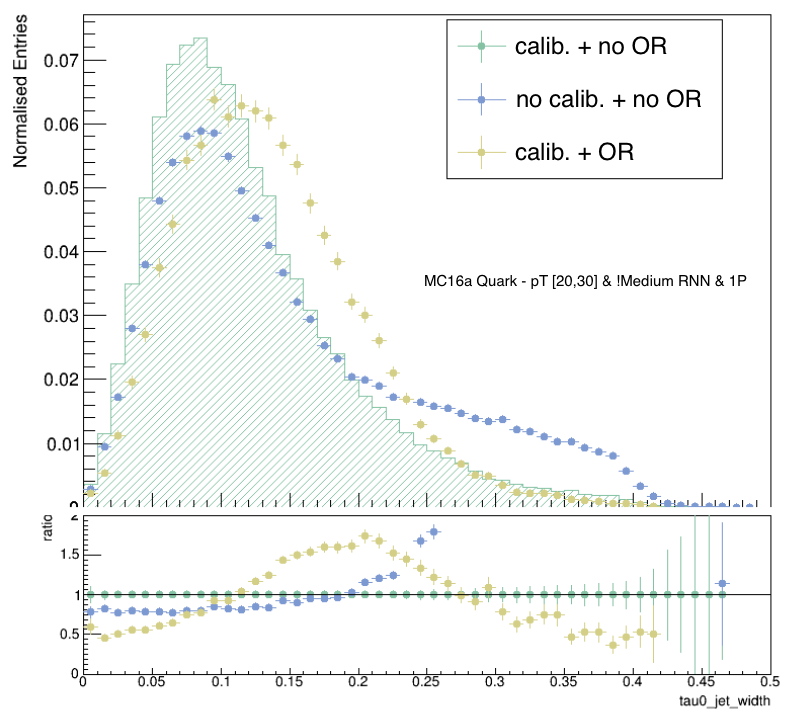
\includegraphics[width=0.7\textwidth]{FakeTau/DxAOD/quark_OR_comp}
		\caption{comparison between samples with (red) and without (black) the \ac{OR} procedure applied.}
	\label{fig:ORvsnoOR}
	\end{figure}	
	
	In this plot the distributions have been normalised to unity only for values of track-based jet width above 0. This is to better display the differences in template shape between the calibrated and un-calibrated distributions since, as shown in the previous section, have significantly different scales when normalised to unity while taking into account the values of track-based jet width of -1. The calibration of the reconstructed tau objects cause a decrease in the of the tail of the distribution, as shown by comparing the green and the blue histograms. 
	This seems to be due to the fact that by applying the \ac{TES} calibration a significant number of low-\pt\ \htau\ that normally populate the tail of the distribution are renormalised in a way that now allows them to fail the track-based jet width requirements, thus also explaining the large increase in track-based jet width values of -1. 
	Thus, the ratio between the two histograms is approximately flat in the bulk of the distributions, with the large shape discrepancy being observed primarily in the tail.
	 By comparing the green and yellow histogram shapes it is clear that the \ac{OR} procedure introduces a shift in the track-based jet width distribution towards higher-\pt\ values. This is due to the fact that lower-\pt\ tracks will generally have "larger cones" and thus have a higher probability of overlapping with other objects. 
	
\subsection*{DAOD Selection}
	\label{sec:DAOD_selection}
	%\ac{DAOD} (also called "derivation") is the name given to \ac{AOD} samples that have also been processed through "derivation selections". These are basic selections applied to samples to allow for analysis use in \ac{ATLAS}.
	 The \ac{ATLAS} experiment has produced many different analysis derivations to cover the full \ac{ATLAS} physics program. 
	For this study only a small specific subset of the available derivations are considered. 
	These are the TAUP3, SUSY11 and HIGG4D2 derivations.
	These derivations have been specifically chosen because the "derivation selections" applied in them do not affect the kinematic properties of the tau leptons, via direct skimming or slimming of the tau containers nor by requesting a minimum \ac{BDT} or \ac{RNN} identification algorithm score requirement. 
	Thus resulting in \ac{DAOD} samples that are completely unbiased by the derivation used. 
	The derivation selection applied in the \ac{DAOD} however limit the possible samples that are produced with these derivations. 
	
	\begin{table}[!hbt]
	\caption{Derived \ac{AOD} selections and samples used. \ac{LP} samples have all been produced using the TAUP3 derivation with the exception of \ac{LP} di-jets.}
	%\documentclass[10pt]{article}
%\usepackage[usenames]{color} %used for font color
%\usepackage{amssymb} %maths
%\usepackage{amsmath} %maths
%\usepackage[utf8]{inputenc} %useful to type directly diacritic characters
%\begin{document}
%\begin{table}[]
\resizebox{\textwidth}{!}{\begin{tabular}{ccc} \hline
\textbf{Derivation} & \textbf{Samples} & \textbf{Selection} \\ \hline \hline
SUSY11 & HP Di-jet & \begin{tabular}[c]{@{}c@{}}single-jet trigger skim \\ and $\tau$ $p_T$ $>$ 15 GeV with 1 or 3 charged tracks\end{tabular} \\\hline
HIGG4D2 & HP Z+jets & \begin{tabular}[c]{@{}c@{}}at least one $\tau$ with $p_T$ $>$ 18 GeV and $\Delta$R $<$ 0.6,\\ non-cosmic ("good") muon~\cite{cite-key} with $p_T$ $>$ 12 GeV,\\ electron with $p_T$ $>$ 15 \gev\ passes:\\ the electromagnetic calorimeter-based isolation~\cite{ele-id} \textit{Medium} working point OR\\ the likelyhood-based identification~\cite{ele_id} \textit{Medium} working point\\ and there is a jet with $p_T$ $>$ 18 GeV\end{tabular} \\ \hline
TAUP3 & \begin{tabular}[c]{@{}c@{}}HP W+jets \\ LP samples*\end{tabular} & \begin{tabular}[c]{@{}c@{}}at least one non-cosmic muon~\cite{cite-key} with $p_T$ $<$ 20 GeV,\\ at least one $\tau$ with $p_T$ $>$ 18 GeV with 1 or 3 charged tracks\\ and at least one primary vertex in event with more than 3 associated tracks\end{tabular} \\ \hline
\end{tabular}}
%\end{table}
%
%\end{document}
	\label{tab:DOAD_selections}
	\end{table}
	Table~\ref{tab:DOAD_selections} shows the skimming used within each derivation and which samples were derived. Different samples were derived using different derivation because the selection applied in the \ac{DAOD} limit the possible samples that can pass the specified selection. 
	For example, TAUP3 \ac{DAOD} can be applied to \Wjets\ samples but will be less efficient on di-jet samples due to the requirement of having at least one tau and one muon present in the event which, due to low multiplicity of real muons in this type of decay, would reduce the statistics of the latter sample significantly.
	
	 \begin{figure}[!hbt]
	\centering
	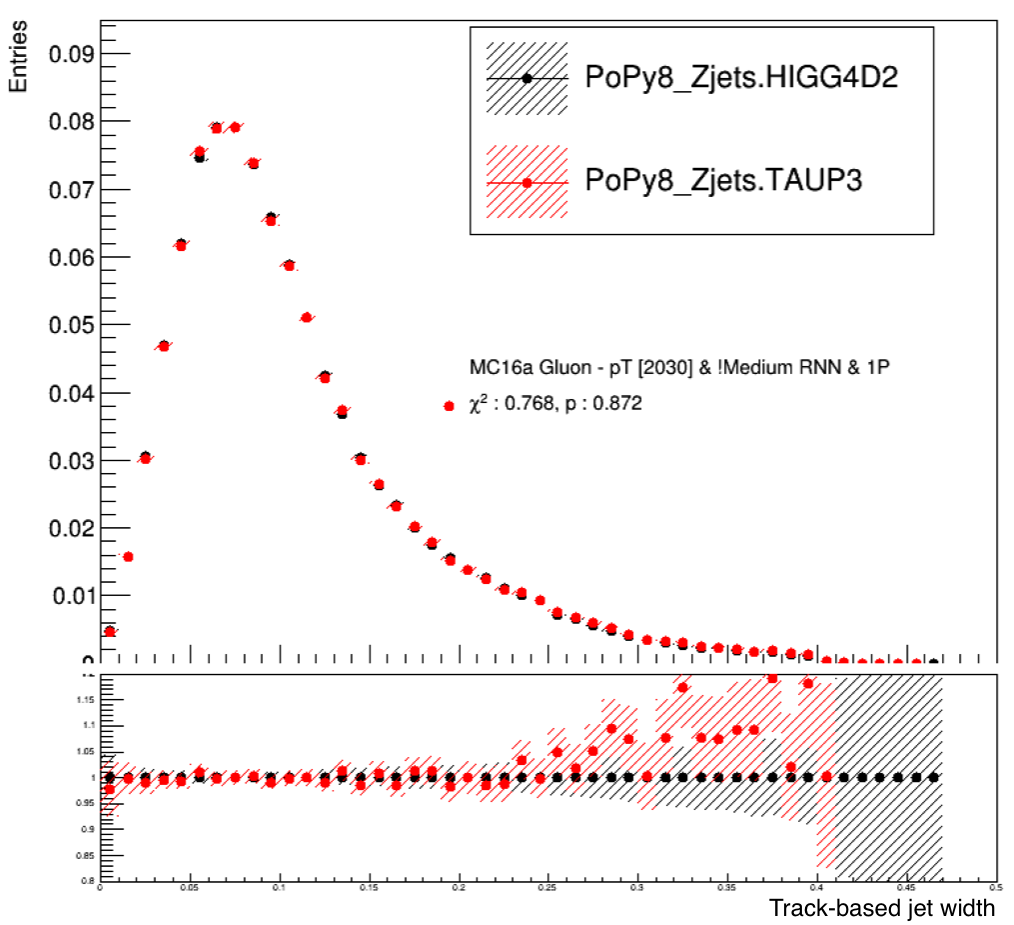
\includegraphics[width=0.7\textwidth]{FakeTau/DxAOD/DAOD_comparison}
	\caption{MC16a tau-faaking gluon initiated jet track based jet width template between HIGG4D2 (black) and TAUP3 (red) Z+jets derivation samples. The $\chi^2$ value with corresponding p-value is shown on plot, indicating a statistical correlation between the two distributions at 95\% CL.}
	\label{fig:DAOD_comparison}
	\end{figure}
	The effect of the different applied \ac{DAOD}s to the same sample is is shown by Figure~\ref{fig:DAOD_comparison}, where the \ac{HP} Z$\rightarrow\mu\mu$ and Z$\rightarrow e e $ are derived using both TAUP3 and HIGG4D2 derivations and are subsequently merged into a unique \Zjets\ sample, for each derivation.
	The track-based jet width distribution for gluon-faking 1 prong \htau\ are derived and plotted against each other using these two different samples in the anti-\textit{Medium} \ac{RNN} region, for \pt\ bin $\in[20,30]$.  
	 The distributions show very good agreement, thus indicating that that there is no apparent bias on the \htau\ reconstructed objects kinematics introduced with the implementation of the \ac{DAOD} selection. 
	
	
	
	%\subsection*{Template universality}
	\section{Proof of concept}
		\label{sec:mctemp}
		Section~\ref{sec:uniffmeth} describes how pure quark or pure gluon regions with (\ie\ regions with $q_f=1$ or $g_f=1$) will have the same respective FF$_q$ and FF$_g$ values, independent of the sample used.  
	%This should hold true even when looking at different samples.
	In turn this indicates that different sample's quark and gluon track based jet width distributions should also be very similar, yet not necessarily identical if we take into account statistical and systematic variations.
	 This property of universality between pure quark and pure gluon regions is referred to as the \ac{FF} and template universality and is a key towards achieving a proof of concept for the universal \ac{FF} method. 
	\subsection{Template universality}
	%Using a selection described in Section ~\ref{subsec:AODsel} the following results are derived.
	% in combination with the requirements highlighted in table ~\ref{tab:FTTF_requierements}, a set of templates can be derived for any given anti-region. 
	 Figure~\ref{fig:AOD_gluon_templates} shows the track based jet width templates separated into the different \pt\ bins described in Section~\ref{subsec:AODsel}, for the 1 prong (top) and 3 prong (bottom) gluon \ftau\ jets with \ac{BDT} score ranging from 0.05 up to the \textit{Medium} \ac{BDT} working point, without \ac{JVT} or trigger requirements from di-jet (black), \Wjets\ (red) and \Zjets\ (green) samples. Only samples that simulate the pileup conditions during 2016 data taking are shown\footnote{Full set of templates for all \pt\ bins, and all average pileup conditions (2016, 2017, and 2018) can be found in Appendix~\ref{app:AODtemplates}}. 
	%Figure ~\ref{fig:AOD_gluon_templates} shows the templates the different \pt bins for 1 prong (left side) and 3 prong (right side) gluon tau-faking jets for Dijet (black), W+jets (red) and Z+jets (green) samples.
	 The templates have been normalised to unity so that the shapes of the templates can be compared without having to worry about the scaling due to the luminosity or cross section of the sample. 
	 The templates have very similar shapes up to the high \pt\ bins where more discrepancies are observed. In these high-\pt\ bins the sample statistics is very low, which allows the event weight to be more significant and thus translate into uneven distributions with large jumps in the data points.
	%In the lower \pt\ bins with higher statistics, the templates match very closely indicating that there is universality between the gluon templates of different samples as suggested by the theory. 
	Figure~\ref{fig:quark_AOD_templates} %and ~\ref{fig:unmatched_AOD_templates}	
	shows the same track-based jet width templates for the quark initiated \ftau\ jet objects.
	The same selection used for the gluon templates is used.% and unmatched tau-faking jets, respectively. 
	These distributions show regions of pure quark and gluon \ftau\ jets, that have been identified and selected using the truth-matching procedure.
	 Because of the consistent shapes of the distributions observed across samples and \pt\ bins, the templates indicate a track-based jet width universality between samples. Some differences are observed in the higher \pt\ bin distributions due to the lower statistics of the samples, making the distribution more susceptible to event weight variations. 
%	\begin{figure}[H]
%	\begin{center}
%\subbottom[]{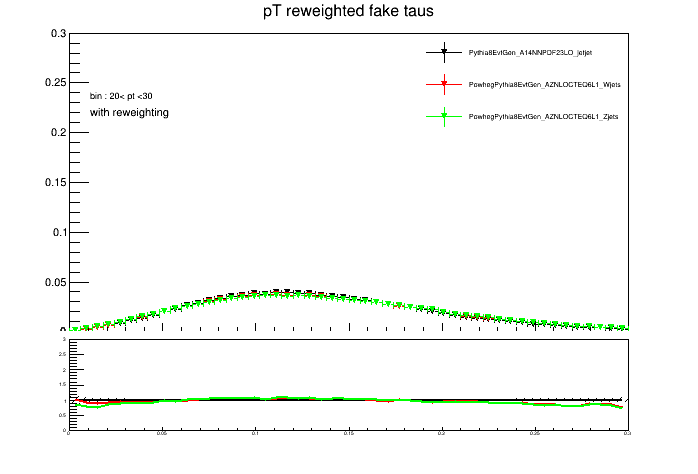
\includegraphics[width=0.3\textwidth]{FakeTau/AOD/MC16a/1p/gluon_Jet_Width_for_All_samples_and_in_bin_[20,30]_for_1_prong.png}}\hspace{0.05\textwidth}
%\subbottom[]{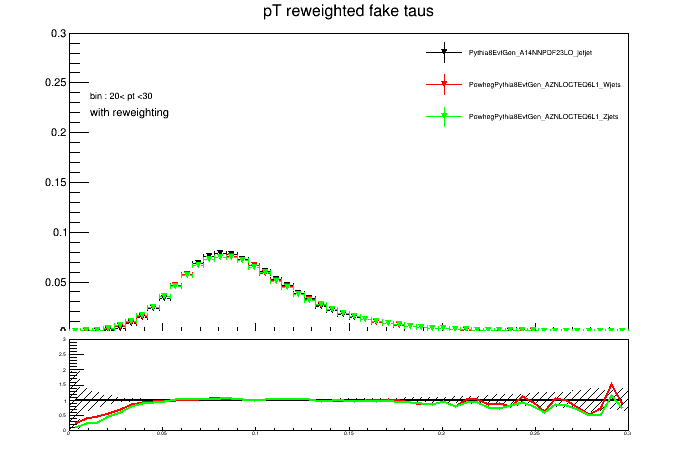
\includegraphics[width=0.3\textwidth]{FakeTau/AOD/MC16a/3p/gluon_Jet_Width_for_All_samples_and_in_bin_[20,30]_for_3_prong.png}}\hspace{0.05\textwidth}
%\subbottom[]{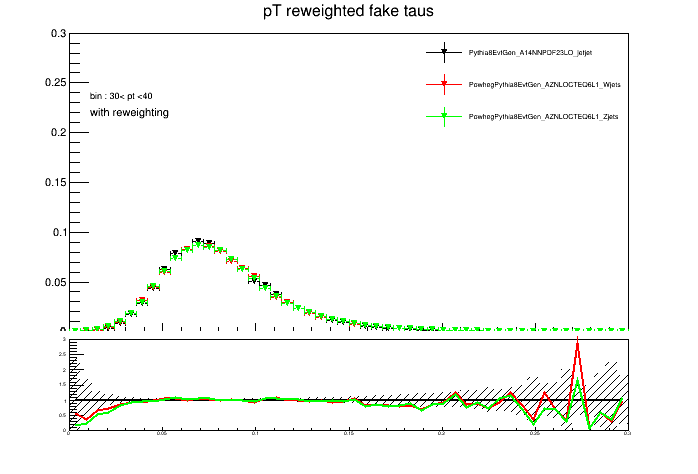
\includegraphics[width=0.3\textwidth]{FakeTau/AOD/MC16a/3p/gluon_Jet_Width_for_All_samples_and_in_bin_[30,40]_for_3_prong.png}}\hspace{0.05\textwidth}
%\subbottom[]{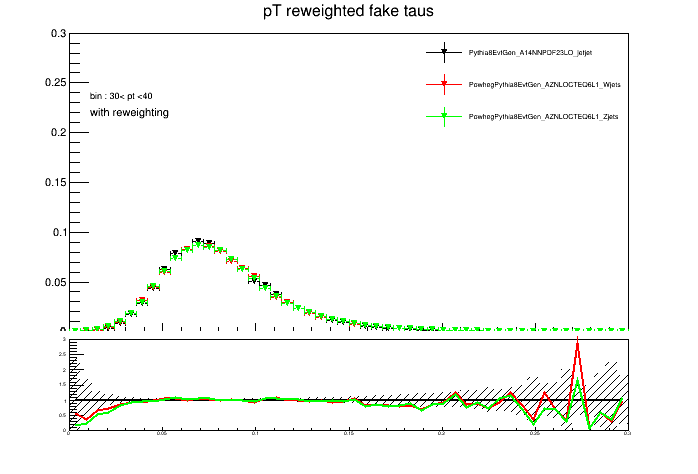
\includegraphics[width=0.3\textwidth]{FakeTau/AOD/MC16a/3p/gluon_Jet_Width_for_All_samples_and_in_bin_[30,40]_for_3_prong.png}}\hspace{0.05\textwidth}
%\subbottom[]{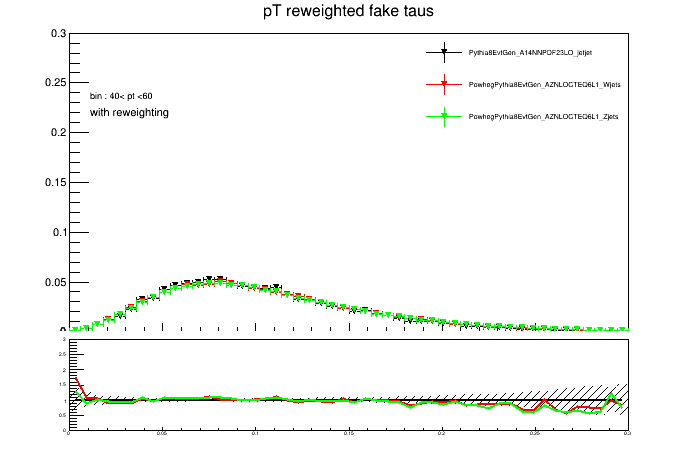
\includegraphics[width=0.3\textwidth]{FakeTau/AOD/MC16a/1p/gluon_Jet_Width_for_All_samples_and_in_bin_[40,60]_for_1_prong.png}}\hspace{0.05\textwidth}
%\subbottom[]{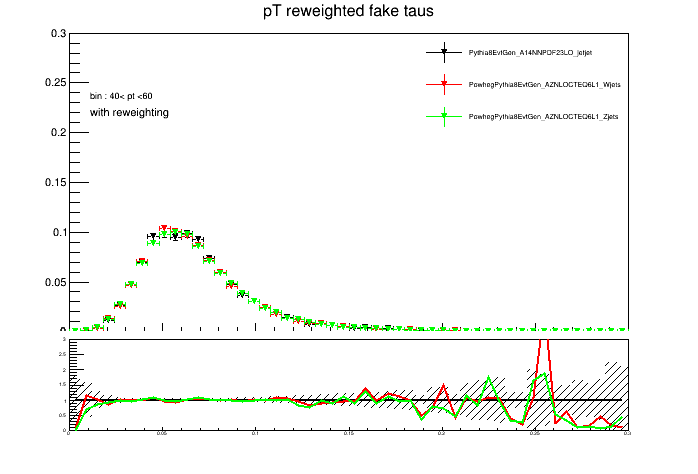
\includegraphics[width=0.3\textwidth]{FakeTau/AOD/MC16a/3p/gluon_Jet_Width_for_All_samples_and_in_bin_[40,60]_for_3_prong.png}}\hspace{0.05\textwidth}
%\subbottom[]{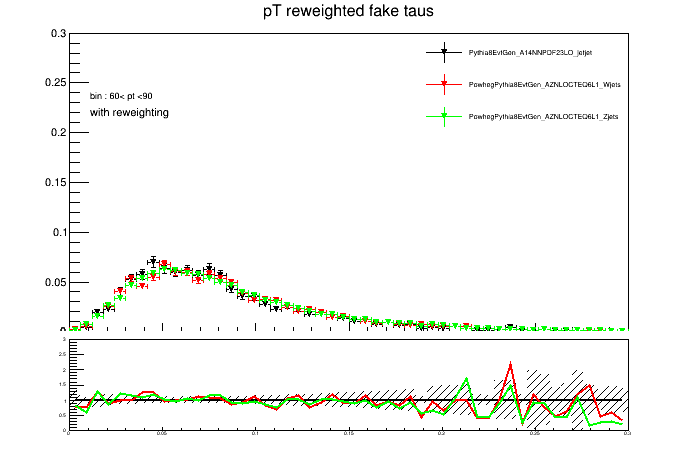
\includegraphics[width=0.3\textwidth]{FakeTau/AOD/MC16a/1p/gluon_Jet_Width_for_All_samples_and_in_bin_[60,90]_for_1_prong.png}}\hspace{0.05\textwidth}
%\subbottom[]{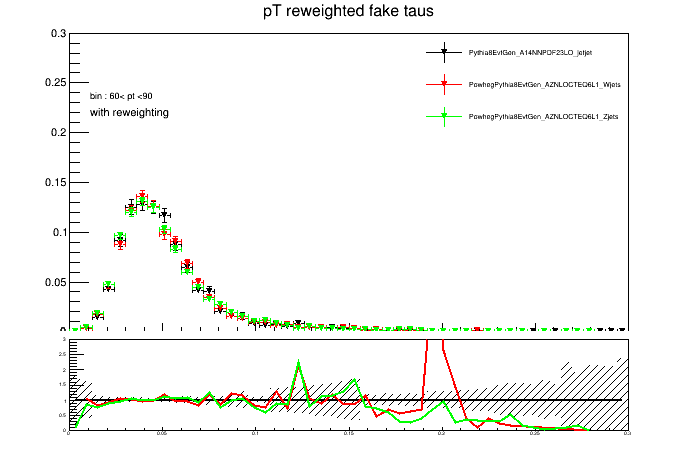
\includegraphics[width=0.3\textwidth]{FakeTau/AOD/MC16a/3p/gluon_Jet_Width_for_All_samples_and_in_bin_[60,90]_for_3_prong.png}}\hspace{0.05\textwidth}
%\subbottom[]{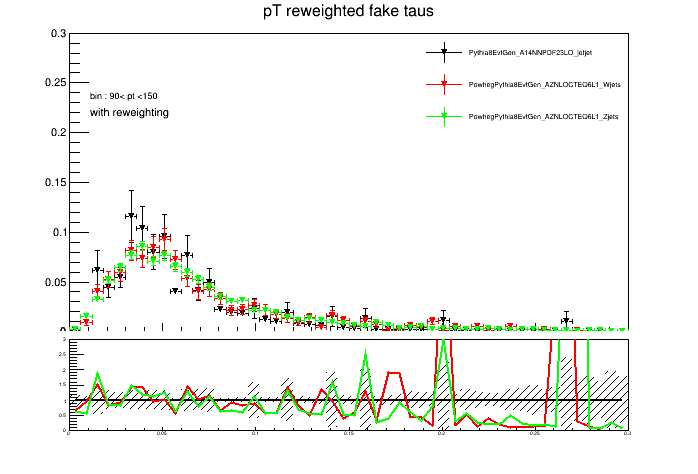
\includegraphics[width=0.3\textwidth]{FakeTau/AOD/MC16a/1p/gluon_Jet_Width_for_All_samples_and_in_bin_[90,150]_for_1_prong.png}}\hspace{0.05\textwidth}
%\subbottom[]{\includegraphics[width=0.3\textwidth]{FakeTau/AOD/MC16a/3p/gluon_Jet_Width_for_All_samples_and_in_bin_[90,150]_for_3_prong.png}}\hspace{0.01\textwidth}
%		\end{center}
%		\caption{Jet Width templates of gluon tau-faking jets separated into \pt\ bins, going from top as the lowest \pt\ bin to bottom being the highest. Left column shows templates for 1 prong tau, while right columns shows 3 prong tau templates.}
%		\label{fig:AOD_gluon_templates}
%	\end{figure}


	\begin{figure}[!hbt]
	\begin{center}
\subbottom[1 prong \htau\ - $20<p_T<30$ GeV]{\includegraphics[width=0.45\textwidth]{FakeTau/AOD/MC16a/1p/gluon_Jet_Width_for_All_samples_and_in_bin_[20,30]_for_1_prong.png}}\hspace{0.05\textwidth}
\subbottom[3 prong \htau\  - $20<p_T<30$ GeV]{\includegraphics[width=0.45\textwidth]{FakeTau/AOD/MC16a/3p/gluon_Jet_Width_for_All_samples_and_in_bin_[20,30]_for_3_prong.png}}\hspace{0.05\textwidth}
\subbottom[1 prong \htau\  - $40<p_T<60$ GeV]{\includegraphics[width=0.45\textwidth]{FakeTau/AOD/MC16a/1p/gluon_Jet_Width_for_All_samples_and_in_bin_[40,60]_for_1_prong.png}}\hspace{0.05\textwidth}
\subbottom[3 prong \htau\  - $40<p_T<60$ GeV]{\includegraphics[width=0.45\textwidth]{FakeTau/AOD/MC16a/3p/gluon_Jet_Width_for_All_samples_and_in_bin_[40,60]_for_3_prong.png}}\hspace{0.05\textwidth}
\subbottom[1 prong \htau\  - $90<p_T<150$ GeV]{\includegraphics[width=0.45\textwidth]{FakeTau/AOD/MC16a/1p/gluon_Jet_Width_for_All_samples_and_in_bin_[90,150]_for_1_prong.png}}\hspace{0.05\textwidth}
\subbottom[3 prong \htau\ - $90<p_T<150$ GeV]{\includegraphics[width=0.45\textwidth]{FakeTau/AOD/MC16a/3p/gluon_Jet_Width_for_All_samples_and_in_bin_[90,150]_for_3_prong.png}}\hspace{0.05\textwidth}
		\end{center}
		\caption{Track based jet width templates of gluon initiated \ftau\ jets. Separated into \pt\ bins of 20-30 \gev, 40-60 \gev\ and 90-150 \gev\ going from top to bottom. Left column row shows templates for 1 prong tau, and right column for the 3 prong tau.}
		\label{fig:AOD_gluon_templates}
	\end{figure}
	
	
%		\begin{figure}[H]
%	\begin{center}
%\subbottom[]{\includegraphics[width=0.4\textwidth]{FakeTau/AOD/MC16a/1p/quark_Jet_Width_for_All_samples_and_in_bin_[20,30]_for_1_prong.png}}\hspace{0.05\textwidth}
%\subbottom[]{\includegraphics[width=0.4\textwidth]{FakeTau/AOD/MC16a/3p/quark_Jet_Width_for_All_samples_and_in_bin_[20,30]_for_3_prong.png}}\hspace{0.05\textwidth}
%\subbottom[]{\includegraphics[width=0.4\textwidth]{FakeTau/AOD/MC16a/1p/quark_Jet_Width_for_All_samples_and_in_bin_[30,40]_for_1_prong.png}}\hspace{0.05\textwidth}
%\subbottom[]{\includegraphics[width=0.4\textwidth]{FakeTau/AOD/MC16a/3p/quark_Jet_Width_for_All_samples_and_in_bin_[30,40]_for_3_prong.png}}\hspace{0.05\textwidth}
%\subbottom[]{\includegraphics[width=0.4\textwidth]{FakeTau/AOD/MC16a/1p/quark_Jet_Width_for_All_samples_and_in_bin_[40,60]_for_1_prong.png}}\hspace{0.05\textwidth}
%\subbottom[]{\includegraphics[width=0.4\textwidth]{FakeTau/AOD/MC16a/3p/quark_Jet_Width_for_All_samples_and_in_bin_[40,60]_for_3_prong.png}}\hspace{0.05\textwidth}
%\subbottom[]{\includegraphics[width=0.4\textwidth]{FakeTau/AOD/MC16a/1p/quark_Jet_Width_for_All_samples_and_in_bin_[60,90]_for_1_prong.png}}\hspace{0.05\textwidth}
%\subbottom[]{\includegraphics[width=0.4\textwidth]{FakeTau/AOD/MC16a/3p/quark_Jet_Width_for_All_samples_and_in_bin_[60,90]_for_3_prong.png}}\hspace{0.05\textwidth}
%\subbottom[]{\includegraphics[width=0.4\textwidth]{FakeTau/AOD/MC16a/1p/quark_Jet_Width_for_All_samples_and_in_bin_[90,150]_for_1_prong.png}}\hspace{0.05\textwidth}
%\subbottom[]{\includegraphics[width=0.4\textwidth]{FakeTau/AOD/MC16a/3p/quark_Jet_Width_for_All_samples_and_in_bin_[90,150]_for_3_prong.png}}\hspace{0.05\textwidth}
%		\end{center}
%		\caption{Jet Width templates of quark tau-faking jets separated into \pt\ bins, going from top as the lowest \pt\ bin to bottom being the highest. Left column shows templates for 1 prong tau, while right columns shows 3 prong tau templates.}
%	\label{fig:quark_AOD_templates}
%	\end{figure}	
	
			\begin{figure}[!hbt]
	\begin{center}
\subbottom[1 prong \htau\ - $20<p_T<30$ GeV]{\includegraphics[width=0.45\textwidth]{FakeTau/AOD/MC16a/1p/quark_Jet_Width_for_All_samples_and_in_bin_[20,30]_for_1_prong.png}}\hspace{0.05\textwidth}
\subbottom[3 prong \htau\ - $20<p_T<30$ GeV]{\includegraphics[width=0.48\textwidth]{FakeTau/AOD/MC16a/3p/quark_Jet_Width_for_All_samples_and_in_bin_[20,30]_for_3_prong.png}}\hspace{0.05\textwidth}
\subbottom[1 prong \htau\ - $40<p_T<60$ GeV]{\includegraphics[width=0.45\textwidth]{FakeTau/AOD/MC16a/1p/quark_Jet_Width_for_All_samples_and_in_bin_[40,60]_for_1_prong.png}}\hspace{0.05\textwidth}
\subbottom[3 prong \htau\ - $40<p_T<60$ GeV]{\includegraphics[width=0.45\textwidth]{FakeTau/AOD/MC16a/3p/quark_Jet_Width_for_All_samples_and_in_bin_[40,60]_for_3_prong.png}}\hspace{0.05\textwidth}
\subbottom[1 prong \htau\ - $90<p_T<150$ GeV]{\includegraphics[width=0.45\textwidth]{FakeTau/AOD/MC16a/1p/quark_Jet_Width_for_All_samples_and_in_bin_[90,150]_for_1_prong.png}}\hspace{0.05\textwidth}
\subbottom[3 prong \htau\ - $90<p_T<150$ GeV]{\includegraphics[width=0.45\textwidth]{FakeTau/AOD/MC16a/3p/quark_Jet_Width_for_All_samples_and_in_bin_[90,150]_for_3_prong.png}}\hspace{0.05\textwidth}
		\end{center}
		\caption{Track based jet width templates of quark initiated \ftau\ jets. Separated into \pt\ bins of 20-30 \gev, 40-60 \gev\ and 90-150 \gev\ going from top to bottom. Left column row shows templates for 1 prong tau, and right column for the 3 prong tau.}
	\label{fig:quark_AOD_templates}
	\end{figure}	
%\begin{figure}[!hbt]
%	\begin{center}
%\subbottom[]{\includegraphics[width=0.4\textwidth]{FakeTau/AOD/MC16a/1p/unmatched_Jet_Width_for_All_samples_and_in_bin_[20,30]_for_1_prong.png}}\hspace{0.05\textwidth}
%\subbottom[]{\includegraphics[width=0.4\textwidth]{FakeTau/AOD/MC16a/3p/unmatched_Jet_Width_for_All_samples_and_in_bin_[20,30]_for_3_prong.png}}\hspace{0.05\textwidth}
%\subbottom[]{\includegraphics[width=0.4\textwidth]{FakeTau/AOD/MC16a/3p/unmatched_Jet_Width_for_All_samples_and_in_bin_[30,40]_for_3_prong.png}}\hspace{0.05\textwidth}
%\subbottom[]{\includegraphics[width=0.4\textwidth]{FakeTau/AOD/MC16a/3p/unmatched_Jet_Width_for_All_samples_and_in_bin_[30,40]_for_3_prong.png}}\hspace{0.05\textwidth}
%\subbottom[]{\includegraphics[width=0.4\textwidth]{FakeTau/AOD/MC16a/1p/unmatched_Jet_Width_for_All_samples_and_in_bin_[40,60]_for_1_prong.png}}\hspace{0.05\textwidth}
%\subbottom[]{\includegraphics[width=0.4\textwidth]{FakeTau/AOD/MC16a/3p/unmatched_Jet_Width_for_All_samples_and_in_bin_[40,60]_for_3_prong.png}}\hspace{0.05\textwidth}
%\subbottom[]{\includegraphics[width=0.4\textwidth]{FakeTau/AOD/MC16a/1p/unmatched_Jet_Width_for_All_samples_and_in_bin_[60,90]_for_1_prong.png}}\hspace{0.05\textwidth}
%\subbottom[]{\includegraphics[width=0.4\textwidth]{FakeTau/AOD/MC16a/3p/unmatched_Jet_Width_for_All_samples_and_in_bin_[60,90]_for_3_prong.png}}\hspace{0.05\textwidth}
%\subbottom[]{\includegraphics[width=0.4\textwidth]{FakeTau/AOD/MC16a/1p/unmatched_Jet_Width_for_All_samples_and_in_bin_[90,150]_for_1_prong.png}}\hspace{0.05\textwidth}
%\subbottom[]{\includegraphics[width=0.4\textwidth]{FakeTau/AOD/MC16a/3p/unmatched_Jet_Width_for_All_samples_and_in_bin_[90,150]_for_3_prong.png}}\hspace{0.01\textwidth}
%		\end{center}
%		\caption{Jet Width templates of unmatched tau-faking jets separated into \pt\ bins, going from top as the lowest \pt\ bin to bottom being the highest. Left column shows templates for 1 prong tau, while right columns shows 3 prong tau templates.}
%		
%	\label{fig:unmatched_AOD_templates}
%	\end{figure}			
	% \subsubsection*{RNN templates}
	
	Figure~\ref{fig:qgu_jetwidth_template} shows the track based jet width template for the quark, gluon and un-matched tau-faking jets. A good separation is observed between the quark and gluon templates, as expected. However, very similar templates are observed in the lower \pt\ bins of the di-jet sample between the gluon and un-matched candidates. 
	This suggests that the un-matched candidates could be used as a statistical supplement to the gluon template for some of the samples where the templates match.	
	%Furthermore, the templates for the different campaigns have to be derived separately.
	 As explained in Section~\ref{subsec:pt_reweight}, the different pileup condition, simulated for the \ac{MC} samples to reflect the Run-2 data taking period, have a direct affect the jet width templates of the tau-faking partons. In particular the un-matched candidates are heavily affected by the pileup conditions and multiplicity of the  studied sample. This is particularly evident in the different track based jet width distributions of the un-matched candidates between the \Zjets\ and di-jet sample. The effect of pileup on the shape of the un-matched candidates track based jet width templates will be discussed in more details in Section~\ref{sec:DAODtemplates}.
	\begin{figure}[!hbt]
		\begin{center}
			\subbottom[]{
				\includegraphics[width=0.45\textwidth]{FakeTau/AOD/MC16a/AOD_qgu_Zjets}}\hspace{0.03\textwidth}
			\subbottom[]{
				\includegraphics[width=0.45\textwidth]{FakeTau/AOD/MC16a/AOD_qgu_dijet}}\hspace{0.03\textwidth}
		\end{center}
		\caption{Distributions of track-based jet width for quark, gluon and un-matched candidates in Z+jet (left) and dijet (right) samples. Ratio plot between the quark and other samples partons is shown in the bottom plot of the diagrams.}
	\label{fig:qgu_jetwidth_template}
	\end{figure}	
	
	It is important to note that the \ac{RNN} identification algorithm was changed to be the recommended identifier algorithm in mid-2019.
	 Due to this, the full set of templates has been derived for both \ac{BDT} and \ac{RNN} scores, to allow for the study of the effect of both identifiers and subsequent derivation of \ac{FF}s using both algorithms. 
	Appendix~\ref{app:AODtemplates} contains the full set of jet width templates derived  for regions with minimum \ac{RNN} score of 0.01 up to \textit{Medium} \ac{RNN} working point, without \ac{JVT} or trigger requirement for the di-jet, \Wjets\ and \Zjets\ samples.
	%In this section a similar set of templates are shown, with the same exact selections as above with the exception of the identifier algorithms which has been changed to the RNN algorithm. Therefore, the following results are derived for the 1 and 3 prong \htau\ with minimum RNN score of 0.01 for the Medium RNN anti-region, without JVT or trigger requirements from Dijet, W+jet and Z+jet MC16a samples.
	\subsection{FF universality}
	\begin{figure}[!hbt]
		\begin{center}
			\subbottom[]{
				\includegraphics[width=0.45\textwidth]{FakeTau/AOD/MC16a/pT/1_Prong_Medium_quark_pT_[20,30]}}\hspace{0.05\textwidth}
			\subbottom[]{
				\includegraphics[width=0.45\textwidth]{FakeTau/AOD/MC16a/pT/3_Prong_Medium_quark_pT_[40,60]}}\hspace{0.05\textwidth}
			\subbottom[]{
				\includegraphics[width=0.45\textwidth]{FakeTau/AOD/MC16a/pT/1_Prong_Medium_gluon_pT_[20,30]}}\hspace{0.05\textwidth}
			\subbottom[]{
				\includegraphics[width=0.45\textwidth]{FakeTau/AOD/MC16a/pT/3_Prong_Medium_gluon_pT_[40,60]}}\hspace{0.05\textwidth}
			\subbottom[]{
				\includegraphics[width=0.45\textwidth]{FakeTau/AOD/MC16a/pT/1_Prong_Medium_unmatched_pT_[20,30]}}\hspace{0.05\textwidth}
			\subbottom[]{
				\includegraphics[width=0.45\textwidth]{FakeTau/AOD/MC16a/pT/3_Prong_Medium_unmatched_pT_[40,60]}}\hspace{0.05\textwidth}
		\end{center}
		\caption{Distribution of visible \htau \pt\ for quark (top) and gluon (middle)  and un-matched (bottom) tau-faking jet candidates pass and fail  region for "Medium" BDT working point in \pt\ bins 20-30 GeV (left) and 40-60 GeV (right). Bottom plot shows corresponding FF values.}
	\label{fig:pT_AOD_dist_FF}
	\end{figure}	
	Using the same selections as in the previous section the \pt\ distributions for the quark, gluon and un-matched candidates in the \Zjets, \Wjets\ and di-jet samples can be derived, as well as the corresponding \ac{FF} values as a function of leading \htau\ \pt. 
	Figure~\ref{fig:pT_AOD_dist_FF} shows the binned \pt\ distribution for the leading \htau\ faking quark, gluon and un-matched initiated jet candidate that pass (solid line) and fail (dotted line) the \textit{Medium} \ac{BDT} identifier working point, with corresponding \ac{FF} values binned into the appropriate \pt\ bins for each sample. 
	As shown in the figure, the \ac{FF} values are consistent between samples, albeit with some small differences due to kinematic and statistical effects of the sample, and seem to be \pt\ dependent\footnote{Corresponding \pt\ and \ac{FF} distributions derived using the \ac{RNN} identifier algorithm can be found in Appendix~\ref{app:AODtemplates}. A similar behaviour of the \ac{FF} is found for the \ac{RNN} identifier based distributions to the ones shown in this section.}.
	As mentioned in previously, even though different samples are being considered, since we are observing a pure quark, gluon, or un-matched region then the \ac{FF} is expected to be consistent between samples. This shows that  there seems to also be \ac{FF} universality as predicted by the universal \ac{FF} method.
	\section{DAOD Templates}
	\label{sec:DAODtemplates}
	For the fitting procedure the quark, gluon and un-matched candidate templates are need from different processes and samples. 
	To account for the \htau\ biases introduced by derivations, the quark, gluon and un-matched candidate templates have also been derived using \ac{DAOD} samples.   
	\subsection{Quark templates}
	\label{subsec:FTTFquark}
	%Using the \ac{DAOD} samples the quark initiated tau-faking jets track-based jet width templates can be studied in more detail. 
	Figure~\ref{fig:quark_and_bjet} shows the quark distribution between di-jet,  \Zjets\ and \ttbar\ samples for the 1 prong \htau\ candidates that fail the \ac{RNN} identification working point, with \pt\ bin $\in[20,30]$. 
	Significant agreement is observed between the di-jet and \Zjets\ templates but a large shift in the track-based jet width distribution is observed in the \ttbar\ sample.
	\begin{figure}[!hbt]
	\begin{center}
	\subbottom[]{
	\includegraphics[width=0.49\textwidth]{FakeTau/DxAOD/quark+bjet}\label{fig:quark_and_bjet}}\hspace{0.0\textwidth}
	\subbottom[]{
	\includegraphics[width=0.49\textwidth]{FakeTau/DxAOD/quark+nobjet}\label{fig:quark_nobjet}}\hspace{0.0\textwidth}
	\end{center}
	\caption{Quark initiated tau-faking jets track-based jet width distribution between di-jet (black), \Zjets\ (red) and \ttbar\ (green) samples. All histograms have been normalised to unity and have been re-weighted to the di-jet Quark \pt\ distribution. The $\chi^2$ value with corresponding p-values (with respect to the di-jet distribution) are shown for each histogram.}
\end{figure}				
	
	Upon closer inspection of the quark initiated \ftau\ jets, the track-based jet width distribution was found to be directly dependent on quark-type, where the mean value of track-based jet width increases for increasingly heavier quarks. 
	For a $b$-jet abundant sample such as is the \ttbar, this translates to a general shift of the track-based jet width distribution towards larger values for all \pt\ bins.
%	\begin{figure}[!hbt]
%	\centering
%	\includegraphics[width=0.6\textwidth]{FakeTau/DxAOD/quark+nobjet}
%	\caption{Quark-initiated tau-faking jets, excluding b-jets, track-based jet width distribution between di-jet (black), \Zjets\ (red) and \ttbar\ (green) samples. All histograms have been normalised to unity and have been re-weighted to the di-jet quark \pt\ distribution. The $\chi^2$ value with corresponding p-values (with respect to the di-jet distribution) are shown for each histogram.}
%	\label{fig:quark_nobjet}
%\end{figure}		
	Figure~\ref{fig:quark_nobjet} shows the track-based jet width templates for quark-initiated \ftau\ jets in the di-jet, \Zjets\ and \ttbar\ samples using the same selection used in Figure~\ref{fig:quark_and_bjet}, but now without taking into account the track-based jet width values deriving from the $b$-jet partons.
	The resulting templates show good agreement, with little change observed in the \Zjets\ and di-jet templates (which is expected), while a large shift towards smaller values of track-based jet widths is observed in the \ttbar\ template that allows for better agreement to the di-jet and \Zjets\ templates. 
	%\subsection{Bottom Quark templates}		
    %\label{subsec:FTTFbjet}
	\subsection{Gluon templates}
	\label{subsec:FTTFgluon}
	Similarly to the previous section the gluon templates have been studied in closer detail. 
	Figure~\ref{fig:gluon_DxAOD_template} left-hand side plot (a) shows the track-based jet width distributions between the \textsc{Pythia 8} di-jet, \textsc{Powheg}+\textsc{Pythia 8} Z+jet and \textsc{Sherpa 221} \Vjets\ samples. 
	A significant shift is observed between the templates, with the \textsc{Sherpa 221} (\textsc{Powheg}+\textsc{Pythia 8}) sample being shifted towards lower (higher) track-based jet width average values. 
	\begin{figure}[!hbt]
	\begin{center}
			\subbottom[]{
	\includegraphics[width=0.49\textwidth]{FakeTau/DxAOD/gluon_DxAOD_template}}\hspace{0.0\textwidth}
		\subbottom[]{
	\includegraphics[width=0.49\textwidth]{FakeTau/DxAOD/gluon_shiftFactor}}\hspace{0.0\textwidth}
	\end{center}
	\caption{Gluon-initiated tau-faking jets, track-based jet width distribution between di-jet (black), Z+jets (red) and \Vjets\ (green) samples. All histograms have been normalised to unity and have been re-weighted to the di-jet Gluon \pt\ distribution. The $\chi^2$ value with corresponding p-values (with respect to the di-jet distribution) are shown for each histogram.}
	\label{fig:gluon_DxAOD_template}
\end{figure}	

	This effect is caused by the different generator used to simulate the parton level objects. Depending on the \ac{PDF} set and parton showering used at generator level, different kinematic distributions for the parton objects are obtained, which in turn affect the kinematic properties of the partons which translate to a shift in the shape of the track-based jet width distribution. 
	To account for this effect a "shift factor" is derived. 
	By shifting the template of the \Zjets\ template by some fractional amount (which will be referred to as the "shift factor") it is possible to obtain an optimised track-based jet width distribution that minimises the $\chi^2$ value between the di-jet and \Zjets\ samples template shapes, as shown in the plot on the right (b) of Figure~\ref{fig:gluon_DxAOD_template}. 
	The derived "shift factor" can thus be used a systematic error to account for the different generators that have been used to produce the different set of samples. 
	This systematic error should therefore be included when evaluating the errors associated with the fitting procedure. 
%	\begin{figure}[!hbt]
%	\centering
%	\includegraphics[width=0.7\textwidth]{FakeTau/DxAOD/gluon_shiftFactor}
%	\label{fig:gluon_shiftFactor}
%	\caption{Gluon-initiated tau-faking jets, track-based jet width distribution between di-jet (black), Z+jets (red) and V+jets (green) samples. All histograms have been normalised to unity and have been re-weighted to the di-jet Gluon \pt\ distribution. The $\chi^2$ value with corresponding p-values (with respect to the di-jet distribution) are shown for each histogram.}
%\end{figure}	

	\subsection{Un-matched jet templates}
	As described in Section~\ref{subsec:AODsel}, the un-matched candidates are defined as jet objects which either fail the truth matching procedure or if no seeding jet is found for the reconstructed \htau. 
	The un-matched candidates have also been found to be primarily composed of pile-up jets. 
	This indicates that the kinematic distributions of the un-matched candidates should be heavily affected by the selection used on the derivation sample.
	The derivation selection used on the di-jet sample will by construction, due to the low threshold requirement of having to pass a single-jet trigger and have a reconstructed \htau\ for it to be accepted, be more prone to contain pile-up jets in its events. 
	Inversely, the derivation selections used for the \Zjets\ and \ttbar\ samples, which only require one muon and one \htau\ for the event to be accepted, will have a lower probability of containing pile-up jets in the final stored events. 
	This effect is clearly shown in Figure~\ref{fig:unmatched_DxAOD_template}, which shows the track-based jet width distributions between the SUSY11 di-jet, HIGG4D2 \Zjets\ and TAUP3 \ttbar\ samples by the black, red and green points respectively. 
	The plot shows a large discrepancy in the shape of the distributions between the di-jet and \Zjets. This clearly indicates the effect that pile-up jets have on the shape of the un-matched candidates track-based jet width templates. The derivation used has a clear impact on the track based jet width template shape of the un-matched candidates, and must therefore be taken into account in the fit. The un-matched candidates shape will differ significantly depending on the selection used and must thus be taken into account when fitting the \ac{MC} templates to a data region to derive the appropriate quark fraction.
	\label{subsec:FTTFunmatch}
	\begin{figure}[!hbt]
	\centering
	\includegraphics[width=0.6\textwidth]{FakeTau/DxAOD/un-matched_DxAOD_template}
	\caption{Un-matched candidate-initiated tau-faking jets track-based jet width distribution between di-jet (black), \Zjets\ (red) and \ttbar\ (green) samples. All histograms have been normalised to unity and have been re-weighted to the di-jet un-matched \pt\ distribution. The $\chi^2$ value with corresponding p-values (with respect to the di-jet distribution) are shown for each histogram.}
	\label{fig:unmatched_DxAOD_template}
	\end{figure}	
	
	
	
	\section{Fitting Procedure and Tool development}
	The \ac{ATLAS} collaboration is currently developing the \ac{TFFT}~\cite{TFFT} as a single executable in the \ac{ATLAS} analysis program \textsc{Athena 21.2}~\cite{Calafiura:2005zz}. 
	The aim of the tool is to perform "on-the-fly" interpolation for any user-given \ac{SR} that fails the identification classier working point of interest, to derive the corresponding tau \ac{FF} values with associated uncertainties.
	The workflow of the \ac{TFFT}, as well as the required inputs and output are shown in Figure~\ref{fig:TFFT}. The \ac{TFFT} requires the user to provide the \pt\ and jet width histograms for the relevant \ac{SR}. 
	The \ac{ATLAS} dedicated task-force in charge of providing methods components and tools for the determination of the \ftau\ background, which has also been developing the \ac{TFFT}, has been working towards the preparation of the other required inputs for the tool. 
	The provided inputs include the data region and \ac{MC} parton \pt\ and jet widths templates. 
	The \ac{TFFT} performs the \pt\ re-weighting on given jet width templates (discussed in Section~\ref{sec:DAODtemplates}), determines the quark fraction of the input sample, derives the \ac{FF} by interpolation with systematic error calculation.
	\label{sec:TFFT}
	\begin{figure}[!hbt]
	\centering
	\includegraphics[width=0.8\textwidth]{FakeTau/TFFT}
	\caption{Illustration of general workflow of \ac{TFFT}. The \ac{TFFT} requires histograms of \pt\ and jet widths from the user as inputs to the tool. The dedicated \ac{ATLAS} task-force provides the \pt\ and jet width histograms for data-region and \ac{MC} partons inputs required for the interpolation and quark fraction fitting.}
	\label{fig:TFFT}	
	\end{figure}
	
	\subsection*{Quark Fraction determination}
	The quark fraction is determined by a fit to data using the quark, gluon and un-matched MC templates as parameters. 
	The discriminating variable used is the track based jet width, as described in Section~\ref{jet_width}. The fitting procedure is performed using a minimum log-likelihood method, implemented using \textsc{HistFactory}~\cite{Cranmer:1456844} for the likelyhood building and \textsc{Minuit}~\cite{James:2296388} for minimization.
	
	To test the fitting procedure a known mixture of Z$\rightarrow\mu\mu$ and multi-jet events was used to derive the fraction of multi-jet events ($\alpha_{MJ}$) in the sample using the tool.
	 The two samples used for this test have been normalised to the number of Z$\rightarrow\mu\mu$ events.
	 The mixture has been set to 60\% Z$\rightarrow\mu\mu$ events and 40\% multi-jet events. 
	Figure~\ref{fig:TFFT_test_alphaMJ} shows the result of the \ac{TFFT} fitting procedure using this sample mixture, not considering systematic constraints or the effect of statistical uncertainty. 
	The fit is able to reproduce the fraction of multi-jet events ($\alpha_{MJ}=0.4$) with a very small $\chi^2$ value, indicating a perfect reconstruction of the known mixture of the two samples. 
	The black dots indicate template of the mixture, while the green and red markers indicate the the Z$\rightarrow\mu\mu$ and multi-jet  events templates, respectively, that have been used to produce the fit, which is shown as the solid blue line on the plot. 
	The ratio of the fitted template and the mixed template is shown in the bottom plot, which is found to be 1 across the whole range of jet width values. 
	This validates the fitting procedure ability to reproduce the correct fraction of multi-jet evens in the sample. 
	\begin{figure}[!hbt]
	\centering
	\includegraphics[width=0.6\textwidth]{FakeTau/TFFT/TFFT_test_alphaMJ}
	\caption{Fit of Z$\rightarrow\mu\mu$ and multi-jet data templates to a known mixture of the two. Fit does not consider any constraint terms describing systematic variations. Templates correspond to one prong, 20-30 \gev\ \htau\ candidates that fail the \textit{Medium} \ac{BDT} working point.}
	\label{fig:TFFT_test_alphaMJ}
	\end{figure}
	
	In order to model the fit results with the addition of systematic uncertainties, the following constraint terms have been tested: 
	\begin{description}
	\item[Flat Systematic Uncertainty:] Log-normal constraint of $\pm$5\% of the bin content of each sample. For this type of systematic $\pm$5\% represents $\pm1\sigma$.
	\item[Shape Shift Uncertainty:] Log-normal constraint of Gaussian variation for each bin centred at 0 with $\sigma$ of 1 for both "up" and "down" variation.
	\item[Template Statistical Uncertainty:] Gaussian constraint that uses a modified version of the Barlow-Beeston method, which cosiders the relative statistical uncertainty for al samples combined. More details can be found in Reference~\cite{BARLOW1993219} for more details.
	\end{description}

	By implementing the aforementioned constraints simultaneously in the fitting procedure, in order to mimic the inclusion of systematic and statistical uncertainties, the templates and fitting can be re-performed for the mixed samples as shown by Figure~\ref{fig:TFFT_test_alphaMJ_unc}. 
	On the left the result of the fit is shown with both Z$\rightarrow\mu\mu$ and multi-jet templates. The right plot shows the pull plot of the included systematic variations. 
	The fit shows a slight increase in error from 1.3\% to 2.5\% with $\chi^2<<1$, which is indicative of an "Asimov" type fit to a precisely know data sample. 
	The "pull" plot indicates that the fit result is consistent with the expectation that the templates are precise, given the known mixture of the data sample.
	 The exception is "fraction multi-jet", which corresponds to the fraction of multi-jet events in the sample. This is due to starting point for both templates being declared as 50\%, thus making this kind of pull expected. 
	 
	\begin{figure}[!hbt]
	\begin{center}
	\subbottom[]{
	\includegraphics[width=0.45\textwidth]{FakeTau/TFFT/TFFT_test_alphaMJ_unc}}\hspace{0.03\textwidth}
	\subbottom[]{
	\includegraphics[width=0.45\textwidth]{FakeTau/TFFT/TFFT_unc_pull}}\hspace{0.03\textwidth}
	\end{center}
	\caption{Left hand plot shows fit of Z$\rightarrow\mu\mu$ and multi-jet data templates to a known mixture of the two. Systematic variations constraint terms have been taken into account when performing fit. Templates correspond to one prong, 20-30 \gev\ \htau\ candidates that fail the \textit{Medium} \ac{BDT} working point. Right hand plot shows "pull" plot of the relevant systematics included in the fitting procedure performed in the left plot.}
	\label{fig:TFFT_test_alphaMJ_unc}
	\end{figure}
	Since the \ac{FF} interpolation contains three unknowns, $\alpha_Z$, $\alpha_{MJ}$ and $\alpha_{SR}$, the fraction fitting procedure is the most important part of the \ac{TFFT}.
	 The fitting procedure performed for the determination of the quark-fraction of a given sample using the calibrated quark, b-jet, gluon and un-matched \htau -faking jet candidate templates is shown in Figure~\ref{fig:TFFT_fit_MC}. 
	 The 20-30 \gev\ \pt\ bin is shown for the candidates that fail the \textit{Medium} \ac{RNN} identification criteria working point. The mixed sample used in this case has a quark fraction ($\alpha_q$) of 50\%. 
	The fit has improved significantly with the inclusion of the un-mathced and b-jet templates as parameters to the fit, resulting in a $\chi^2 < 5$ and a $\alpha_q$=0.512$\pm$0.004.
	It is important to note that appropriate systematic uncertainties need to be identified and implemented into the quark fraction fitting procedure for a proper estimate of the quark fraction and fit to be derived.  
	
		\begin{figure}[!hbt]
	\centering
	\includegraphics[width=0.6\textwidth]{FakeTau/TFFT/TFFT_fit_MC}
	\caption{Fit of Z$\rightarrow\mu\mu$ and multi-jet data templates to a known mixture of the two. Fit does not consider any constraint terms describing systematic variations. Templates correspond to one prong, 20-30 \gev\ \htau\ candidates that fail the \textit{Medium} \ac{RNN} working point.}
	\label{fig:TFFT_fit_MC}
	\end{figure}
	The \ac{TFFT} is therefore showing promising results towards the derivation of \ac{FF} values via template fitting and interpolation. 
	The use track based jet width allows shows some promise in its ability to correctly identify the true quark fraction in a given sample, when derived using the 4 parameter fit derived from \ac{MC}: the quark, gluon and b-jet fake-\htau\ candidate jets, as well as the \ac{MC} pileup template in the form of un-matched candidates.
	There are still aspects that need further investigation such as ambiguities in the definition of the \htau\ candidates, including non-uniformity across different object selection frameworks, which are required to test to the robustness of the fit. Furthermore all systematic uncertainties described in the previous sections need to be fully identified and implemented in the quark fraction fitting procedure. 
	
	\section{Summary}
	\label{sec:summary}
	This chapter presented the strategy and implementation of the universal fake factor method for the estimation of the number of fake tau objects present in any \ac{SR} of interest. 
	The studies and tests done towards the ongoing development of the \ac{TFFT} are also presented, including the currently available inputs provided by the dedicated \ac{ATLAS} task force. 
	The work presented in this chapter has been proposed for presentation at several national conferences, including the \href{https://docs.google.com/document/d/1B4myu9WOYEt-N\_h1xjHOJLjrfHtg734BpJhSb0jal\_0}{Sussex Student Conference 2020}\footnote{ \href{https://docs.google.com/document/d/1B4myu9WOYEt-N\_h1xjHOJLjrfHtg734BpJhSb0jal\_0}{https://docs.google.com/document/d/1B4myu9WOYEt-N\_h1xjHOJLjrfHtg734BpJhSb0jal\_0}}, and is expected to be summarised in a paper by the analysis group conveners.
%	A summary provided input regions as well as ongoing studies is given below;
%	\begin{itemize}
%	\item[] Z+jet data region FF values
%	\item[] Multijet data region FF values
%	\item[] quark templates
%	\item[] b-jet templates
%	\item[] gluon templates
%	\item[] un-matched templates 
%	\item[] Summary of tool fitting procedure using the MC derived parton templates to data. 
%	\end{itemize}